%\documentclass[12pt]{article}
\documentclass[10pt]{sigplanconf}

% The following \documentclass options may be useful:
%
% 10pt          To set in 10-point type instead of 9-point.
% 11pt          To set in 11-point type instead of 9-point.
% authoryear    To obtain author/year citation style instead of numeric.
\usepackage[usenames,dvipsnames]{color}
\usepackage[usenames,dvipsnames,svgnames,table]{xcolor}
\usepackage{mathpartir}
\usepackage{amsmath}
\usepackage{amssymb} 
\usepackage{amsthm}
\usepackage{ stmaryrd }
\usepackage{graphicx}
\usepackage{url}
\newcommand{\TODO}[1]{{\color{red} #1}}
%\usepackage{float}
%\floatstyle{ruled}
%\newfloat{figure}{tp}{lop}
%\floatname{figure}{Listing}

%\usepackage[noindentafter]{titlesec}
%\titlespacing{\section}{0pt}{*0.5}{*0.25}
%\titlespacing{\subsection}{3pt}{*1.5}{*0.25}
%\titlespacing{\subsubsection}{3pt}{*1.5}{*0.25}
%\titlespacing{\paragraph}{0pt}{*0.5}{*1}
\usepackage{textpos}


\newcommand{\delete}[1]{}

\newcommand{\isaprop}[1]{#1 : \mathbf{prop}}
\newcommand{\isaproof}[1]{#1 : \mathbf{proof}}


\newcommand{\jtrue}[1]{#1~{\tt true}}
\newcommand{\jtruep}[2]{#1{:}#2}
\newcommand{\type}[1]{#1~{\tt type}}
\newcommand{\entails}[2]{#1 \vdash #2}
\newcommand{\entailst}[3]{#1 \vdash #2 : #3}
\newcommand{\entailsty}[2]{#1 \vdash \type{#2}}
\newcommand{\entailsf}[4]{#1 ; #2 \vdash #3 : #4}




\newcommand{\oftype}[2]{#1 : #2}
\newcommand{\oftypec}[2]{#1 \sim #2}


\newcommand{\disj}[2]{#1 \vee #2}

\newcommand{\I}{\mbox{-I}}
\newcommand{\E}{\mbox{-E}}



\newcommand{\sequent}[2]{#1 \implies #2}

\newcommand{\seqctxt}[1]{^\ulcorner \!#1 ^\urcorner}



\newcommand{\inl}[1]{{\tt inl}(#1)}
\newcommand{\inr}[1]{{\tt inr}(#1)}
\newcommand{\caseof}[5]{{\tt case}(#1, #2 {.} #3, #4{.}#5)}
\newcommand{\lam}[3]{\lambda #1{:}#2{.}#3}
\newcommand{\Lam}[2]{\Lambda #1{.}#2}
\newcommand{\Allt}[2]{\forall #1{.}#2}
\newcommand{\tap}[2]{#1[#2]}
\newcommand{\ap}[2]{#1\,#2}

\newcommand{\BT}{{\bf 2}}
\newcommand{\true}{{\bf t}}
\newcommand{\false}{{\bf f}}

\newcommand{\listof}[1]{{\bf list}[#1]}
\newcommand{\natlist}{{\bf list}}



\newcommand{\tvar}{\mbox{tvar}}
\newcommand{\absF}{{\rightarrow} \mbox{-F}}
\newcommand{\AbsF}{\forall \mbox{-F}}
\newcommand{\var}{\mbox{var}}
\newcommand{\absI}{{\rightarrow} \I}
\newcommand{\AbsI}{\forall \I}
\newcommand{\absE}{{\rightarrow} \E}
\newcommand{\AbsE}{\forall \E}


\newcommand{\subst}[3]{[#1/#2]#3}
\newcommand{\substc}[3]{[#1/#2]#3}
\newcommand{\substt}[4]{[#1/#2]#3 = #4}
\newcommand{\rename}[3]{[#1 \leftrightarrow #2]#3}



\newcommand{\betared}{\mapsto_{\beta}}
\newcommand{\etared}{\mapsto_{\eta}}
%\newcommand{\reduces}{\rightsquigarrow}
\newcommand{\reduces}{\mapsto}

\newcommand{\natrec}[4]{{\bf rec}(#1, #2, #3.#4)}
\newcommand{\nat}{\omega}
\newcommand{\z}{\mathbf{z}}
\newcommand{\s}[1]{\mathbf{s}(#1)}

\newcommand{\cons}[2]{#1 {:}{:} #2}
\newcommand{\nil}{{\bf nil}}
\newcommand{\listrec}[5]{{\bf lrec}(#1, #2, #3.#4.#5)}
\newcommand{\map}[2]{{\tt map}[#1][#2]}


\newcommand{\val}[1]{#1 \,\,\, {\tt val}}
\newcommand{\final}[1]{#1 \,\,\, {\tt final}}


\newcommand{\HT}[4]{{\bf HT}_{#1}^{#2, #3}(#4)}
\newcommand{\HTN}[4]{{\bf HTN}_{#1}^{#2, #3}(#4)}
\newcommand{\HTS}[3]{{\bf HT}_{#1}^{#2, #3}}
\newcommand{\append}[3]{#1[#2 \mapsto #3]}



\newcommand{\eqfam}[5]{#1 \, #3 \, #2 : #4 [#5]}
\newcommand{\obseq}[3]{#1 \cong #2 : #3}
\newcommand{\admiss}[3]{#1 : #2 \leftrightarrow #3}
\newcommand{\plogeq}[6]{#1 \sim #2 : #3 [ #4 : #5 \leftrightarrow #6]}
\newcommand{\logeq}[5]{#1 \sim #2 : #3 [ #4 ;#5]}


\newcommand{\cloquence}{\textsf{cl.oquence}}

\newcommand{\lamA}{\lambda_{\text{A}}}

\newcommand{\tvarCtx}{\Delta}
\newcommand{\fCtx}{\Sigma}
\newcommand{\itvarCtx}{\Omega}
\newcommand{\iCtx}{\Theta}
\newcommand{\eCtx}{\Gamma}
\newcommand{\etvarCtx}{\Omega}
\newcommand{\fSpec}[3]{\tof{\fvar{#1}}{\kFam{#2}{#3}}}
\newcommand{\fSpecStd}{\fSpec{fam}{\kappaidx}{\Theta}}

\newcommand{\errCtx}{\mathcal{E}}
\newcommand{\famEvalCtx}{\Xi}

% Generic stuff
\newcommand{\pipe}{~\text{\large $\vert$}~}
\newcommand{\splat}[3]{#1_{#2},\ldots,#1_{#3}}
\newcommand{\splatC}[3]{#1_{#2}~~~~\cdots~~~~#1_{#3}}
\newcommand{\splatTwo}[4]{#1_{#3}#2_{#3},~\ldots~, #1_{#4}#2_{#4}}
\newcommand{\substn}[2]{[#1]#2}

% \psi
\newcommand{\psiu}[1]{{\psi_{#1}}}
\newcommand{\psit}[1]{{\psi_{\text{#1}}}}
\newcommand{\psitype}{\psit{type}}
\newcommand{\psiproof}{\psit{proof}}
\newcommand{\psiidx}{\psit{idx}}
\newcommand{\psiidxn}[1]{\psit{idx,#1}}
\newcommand{\psirep}{\psit{rep}}
\newcommand{\psirepn}[1]{\psit{rep,#1}}
\newcommand{\psiden}{\psit{den}}
\newcommand{\psiIT}{\psit{IT}}
\newcommand{\psiarrow}{\psit{arrow}}
\newcommand{\psiprod}{\psit{prod}}
\newcommand{\psiint}{\psit{int}}
\newcommand{\psibool}{\psit{bool}}
\newcommand{\psiprog}{\psit{prog}}
\newcommand{\psiiterm}{\psit{iterm}}

% \delta
\newcommand{\delt}[1]{\delta_{\text{#1}}}
\newcommand{\delrep}{\delt{rep}}

% \kappa
\newcommand{\kappat}[1]{\kappa_{\text{#1}}}
\newcommand{\kappaidx}{\kappat{idx}}

% Expressions
\newcommand{\expr}[1]{{\color{red} #1}}
\newcommand{\elam}[3]{{\lam{#1}{#2}{#3}}}
\newcommand{\evar}[1]{{\textrm{#1}}}
\newcommand{\eapp}[2]{{#1~#2}}
\newcommand{\eop}[4]{{#1.\tvar{#2}\langle#3\rangle(#4)}}

% Types
\newcommand{\tdef}[3]{{\sf def}~\tvar{#1}=#2~{\sf in}~#3}
\newcommand{\tlam}[2]{\lambda#1.#2}
\newcommand{\tvar}[1]{{\textbf{#1}}}
\newcommand{\tapp}[2]{#1(#2)}
\newcommand{\tifeq}[4]{{\sf if}~#1\equiv#2~{\sf then}~#3~{\sf else}~#4}

\newcommand{\tunit}{()}
\newcommand{\tpair}[2]{(#1, #2)}
\newcommand{\tfst}[1]{{\sf fst}~#1}
\newcommand{\tsnd}[1]{{\sf snd}~#1}

\newcommand{\fvar}[1]{\textsc{#1}}
\newcommand{\tfam}[6]{{\sf family}~\fvar{#1}[#2]~::~#3~\{#4 : #5\}~{\sf in}~#6}
\newcommand{\tfamStd}{\tfam{fam}{\kappaidx}{\psirep}{\theta}{\Theta}{\psi}}
\newcommand{\tfamcase}[4]{{\sf famcase}~#1~{\sf of}~#2~{\sf then}~#3~{\sf else}~#4}
\newcommand{\tfamSpec}[5]{{\sf family}~[#2]~::~#3~\{#4 : #5\}}
\newcommand{\tfamSpecStd}{\tfamSpec{fam}{\kappaidx}{\psirep}{\theta}{\Theta}}

\newcommand{\ttype}[2]{{\sf type}[#1]\in#2}
\newcommand{\ttypestd}{\ttype{\psiidx}{\phi}}
\newcommand{\tidx}[1]{{\sf idxof}~#1}
\newcommand{\trepof}[1]{{\sf repof}~#1}

\newcommand{\tden}[2]{\llbracket #1 \sim #2 \rrbracket}
\newcommand{\ttypeof}[1]{{\sf typeof}~#1}
\newcommand{\tvalof}[1]{{\sf valof}~#1}
\newcommand{\terr}{{\sf err}}
\newcommand{\tdencase}[4]{{\sf dencase}~#1~{\sf of}~#2~{\sf then}~#3~{\sf else}~#4}

\newcommand{\titerm}[1]{{\sf iterm}(#1)}
\newcommand{\titype}[1]{{\sf itype}(#1)}

\newcommand{\tconst}[1]{{\sf const}(#1)}
\newcommand{\tOp}[1]{{\sf op}(#1)}

\newcommand{\tprog}[1]{{\sf program}(#1)}

\newcommand{\topsempty}{\cdot}
\newcommand{\tops}[2]{\tvar{#1}=#2}
\newcommand{\topp}[2]{#1; #2}
\newcommand{\Tops}[2]{\tvar{#1} : #2}
\newcommand{\Topp}[2]{#1; #2}
\newcommand{\Toppstd}{\Topp{\Theta'}{\Tops{id}{
			\karrow{
				\kType{\kFamStd}
			}{
				\karrow{
					\splat{\kappa}{1}{m}
				}{
					\kOp{n}
				}
			}
		}}
}

% IL terms
\newcommand{\ivar}[1]{\textrm{#1}}
\newcommand{\ilam}[3]{\lambda #1::#2.#3}
\newcommand{\ifix}[3]{{\sf fix~}#1::#2.#3}
\newcommand{\iapp}[2]{#1~#2}
\newcommand{\ipair}[2]{(#1, #2)}
\newcommand{\ifst}[1]{{\sf fst}~#1}
\newcommand{\isnd}[1]{{\sf snd}~#1}
\newcommand{\iintlit}{n}
\newcommand{\iop}[2]{#1 + #2}
\newcommand{\iIfEq}[4]{{\sf if}~#1\equiv#2~{\sf then}~#3~{\sf else}~#4}
\newcommand{\mvalof}[1]{{\sf valof}(#1)}
\newcommand{\iup}[1]{\uparrow(#1)}

% Internal Types
\newcommand{\darrow}[2]{#1\rightarrow#2}
\newcommand{\dint}{\texttt{int}}
\newcommand{\dpair}[2]{#1\times#2}
\newcommand{\dup}[1]{\uparrow(#1)}
\newcommand{\drepof}[1]{{\sf repof}(#1)}

% Kinds
\newcommand{\kvar}[1]{\textrm{#1}}
\newcommand{\karrow}[2]{#1\rightarrow{#2}}
\newcommand{\kforall}[2]{\forall \kvar{#1}.#2}
\newcommand{\kunit}{\texttt{Unit}}
\newcommand{\kstr}{\texttt{Str}}
\newcommand{\kpair}[2]{#1 \times #2}
\newcommand{\klabel}[1]{\textsc{#1}}
\newcommand{\klabelOf}[2]{\klabel{#1}~{\tt of}~#2}
\newcommand{\kTypeBlur}{\texttt{Type}}
\newcommand{\kType}[1]{\texttt{Type}\in #1}
\newcommand{\kOp}[1]{\texttt{Op}_{#1}}
\newcommand{\kDen}{\texttt{Den}}
\newcommand{\kDenk}[1]{\texttt{Den}[#1]}
\newcommand{\kIdxcase}[1]{{\tt Idxcase}~#1}
\newcommand{\kIType}{\texttt{IType}}
\newcommand{\kITerm}{\texttt{ITerm}}
\newcommand{\kEqProof}[3]{#1 \equiv_{#2} #3}
\newcommand{\kProg}{\texttt{Program}}
\newcommand{\kcasev}{\Omega^n}
\newcommand{\kFam}[2]{{\tt family}[#1]\{#2\}}
\newcommand{\kFamStd}{\kFam{\kappaidx}{\Theta}}
\newcommand{\kFamVar}[1]{\overline{\fvar{#1}}}

% Judgements
\newcommand{\tof}[2]{#1 : #2}
\newcommand{\mtof}[2]{#1 :: #2}
\newcommand{\tentails}[2]{#1 \vdash #2}
\newcommand{\tentailst}[3]{\tentails{#1}{\tof{#2}{#3}}}
\newcommand{\tStdCtx}{\fCtx~\tvarCtx}
\newcommand{\tCtxXF}[1]{\fCtx, #1~\tvarCtx}
\newcommand{\tCtxXT}[1]{\fCtx~\tvarCtx, #1}
%\newcommand{\tCtxXL}[1]{\fCtx~\tvarCtx~\lvarCtx, #1}
\newcommand{\tentailsX}[1]{\tentails{\tStdCtx}{#1}}
\newcommand{\tentailsXt}[2]{\tentailsX{\tof{#1}{#2}}}
\newcommand{\kentails}[2]{#1 \vdash #2}
\newcommand{\kentailsX}[1]{\kentails{\fCtx}{#1}}
\newcommand{\iMkCtx}[3]{#1~#2~#3}
\newcommand{\iStdCtx}{\iMkCtx{\fCtx}{\tvarCtx}{\itvarCtx}}
\newcommand{\ientails}[2]{#1 \vdash #2}
\newcommand{\ientailsX}[1]{\entails{\iStdCtx}{#1}}
\newcommand{\casemap}[2]{#1 : #2}
\newcommand{\mentails}[3]{#1, #2 \vdash #3}
\newcommand{\mentailsX}[1]{\mentails{\tvarCtx}{\itvarCtx}{#1}}
\newcommand{\eentails}[4]{#1~#2~#3 \vdash #4}
\newcommand{\eentailsX}[1]{\eentails{\fCtx}{\tvarCtx}{\etvarCtx}{#1}}
\newcommand{\mtentails}[2]{#1 \vdash #2}
\newcommand{\mtentailsX}[1]{\mtentails{\iCtx}{#1}}
\newcommand{\mtentailsXt}[2]{\mtentails{\iCtx}{\mtof{#1}{#2}}}
\newcommand{\kSimple}[1]{#1~{\sf simple}}
\newcommand{\Tentails}[3]{#1 \vdash_{#2} #3}
\newcommand{\TentailsX}[1]{\Tentails{\fCtx}{\fvar{fam}}{#1}}

% Big-Step Semantics
\newcommand{\tevals}[4]{\entails{#1}{#2 \curlyveedownarrow_{#4} #3}}
\newcommand{\tevalsX}[3]{\tevals{\famEvalCtx}{#1}{#2}{#3}}
\newcommand{\tevalX}[2]{\tevalsX{#1}{#2}{\errCtx}}
\newcommand{\tevalms}[3]{#1 \curlyveedownarrow_{#3} #2}
\newcommand{\tevalm}[2]{\tevalms{#1}{#2}{\errCtx}}
\newcommand{\tevales}[3]{#1 \curlyveedownarrow_{#3} #2}
\newcommand{\tevale}[2]{\tevales{#1}{#2}{\errCtx}}
\newcommand{\noprob}{\text{ok}}
\newcommand{\prob}{!}

% Verification and Translation
\newcommand{\translates}[4]{\entails{#1}{#2 \longrightarrow \tden{#3}{#4}}}

% Compilation Semantics
\newcommand{\compiless}[3]{#1 \Longrightarrow \tden{#2}{#3}}
\newcommand{\compiles}[3]{#1 \Longrightarrow \tden{#2}{#3}}
%\newcommand{\translates}[6]{\entails{#1}{\translatesTo{#2}{#3}{#4}{#5}{#6}}}
\newcommand{\translatesTo}[5]{#1 \longrightarrow \tden{#2}{\ttype{#3}{#4}{#5}{6}{7}}}
\newcommand{\translatesX}[5]{\translates{\eCtx}{#1}{#2}{#3}{#4}{#5}}

\newcommand{\ATT}{AT\&T}
\newtheorem{theorem}{Theorem}%[document]
\newtheorem{lemma}{Lemma}
\newtheorem*{corollary}{Corollary}
\newtheorem*{definition}{Definition}


\usepackage{alltt}
\renewcommand{\ttdefault}{txtt}
\usepackage{color}
\usepackage[usenames,dvipsnames,svgnames,table]{xcolor}
\definecolor{mauve}{rgb}{0.58,0,0.82}
\usepackage{listings}
\lstset{
  language=Python,
  showstringspaces=false,
  formfeed=\newpage,
  tabsize=4,
  commentstyle=\itshape,
  basicstyle=\ttfamily\footnotesize,
  morekeywords={lambda, self, assert, as},
  numbers=left,
  numberstyle=\footnotesize\color{gray}\textsf,
  xleftmargin=2em,
  stringstyle=\color{mauve}
}
\lstdefinestyle{Bash}{
    language={}, 
    moredelim=**[is][\color{blue}\bf\ttfamily]{`}{`},
}
\lstdefinestyle{OpenCL}{
	language=C++,
	morekeywords={kernel, __kernel, global, __global, size_t, get_global_id, sin}
}


\begin{document}
\title{Active Typechecking and Translation}
%
%\authorinfo{~}{~}{~}
\authorinfo{Cyrus Omar\and Nathan Fulton\and Jonathan Aldrich}
       {School of Computer Science\\
        Carnegie Mellon University}
        {\{comar, jonathan.aldrich\}@cs.cmu.edu}   
%
\maketitle
\begin{abstract}
Researchers and domain experts typically describe new language-based abstractions as extensions of an existing  language, but most statically-typed languages are \emph{monolithic}: they do not give users the ability to specify the static and dynamic semantics of new types and operators from within. This has lead to a proliferation of mutually incompatible standalone languages, each built around a small collection of privileged constructs. 
An alternative to this \emph{language-external} approach is to work in an extensible programming language where the compile-time behaviors determining the functionality of new core constructs are provided directly within user libraries. Designing such a \emph{language-internal} extensibility mechanism that is both safe  and expressive is non-trivial. % -- extensions must not weaken the global safety properties of the language, compromise the integrity of the compilation process, or interfere with one other, while remaining flexible enough to admit a range of useful constructs.
This paper introduces a mechanism called active type-checking and translation (AT\&T) that aims to address these  challenges. By building upon type-level computation in a novel way, AT\&T admits user specification of a wide range of compile-time behaviors over a fixed grammar in a safe and modular manner. We discuss two points in the design space: (1) a simple calculus designed to distill the essential concepts and admit formal safety theorems, and (2) a fully-implemented language called Ace that we use to demonstrate the expressive power of AT\&T across several domains, including scientific computing, security, functional programming and object-oriented programming.
\end{abstract}

\category{D.3.2}{Programming Languages}{Language Classifications}[Extensible Languages]
\category{D.3.4}{Programming Languages}{Processors}[Compilers]
\category{F.3.1}{Logics \& Meanings of Programs}{Specifying and Verifying and Reasoning about Programs}[Specification Techniques]
%\keywords
%extensible languages, type-level computation, typed compilation


\section{Introduction}
Programming languages have historically been specified and implemented monolithically. To introduce new primitive constructs, researchers or domain experts have developed a new language or a dialect of an existing language, often with the help of tools like domain-specific language frameworks and compiler generators \cite{fowler2010domain}. 
Unfortunately, using different languages for different components of an application, called a {\it language-oriented approach} \cite{journals/stp/Ward94}, has problems when crossing language boundaries: the external interface of a library must only use constructs that can be expressed in all possible calling languages. \TODO{(talk about typical design using a common language like the JVM)} Thus, any specialized invariants cannot be checked statically, decreasing reliability. It also often requires that developers generate unnatural ``glue'' code, impacting performance and defeating a primary purpose of specialized languages: abstracting these low-level details away from developers.

Extensible programming languages promise to decrease the need for new standalone languages by providing more granular, language-internal support for introducing new primitive constructs (i.e. constructs that cannot be correctly and concisely expressed in terms of existing constructs). By using an extensible language, developers would gain the freedom to choose those constructs most suitable for their problem domain and development discipline. Researchers and domain experts would gain the ability to develop new constructs modularly and distribute them for evaluation by a broader development community without requiring either wholesale adoption of a new language or approval from the maintainers of widely-used languages, who are naturally risk-averse and are unlikely to cater to niche domains. The key difference between the language-external approach, characteristic of language frameworks,  and this language-internal approach, characteristic of extensible languages, is illustrated in Figure \ref{approaches}.
\begin{figure*}
\begin{center}
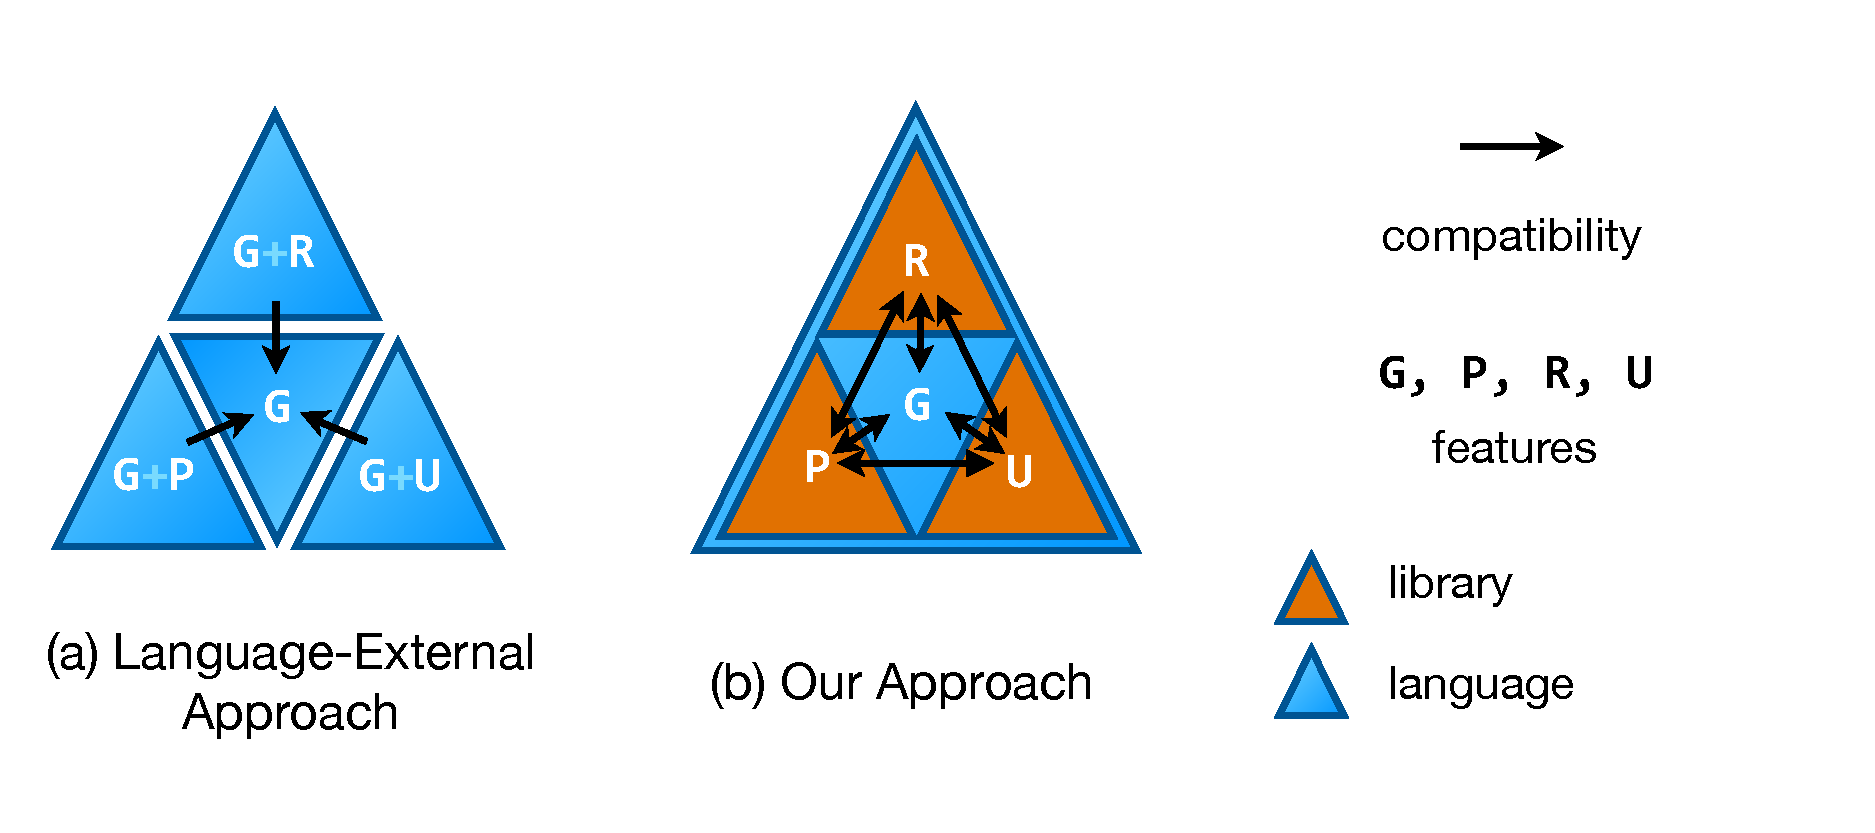
\includegraphics[scale=0.5]{approaches.pdf}
\end{center}
\vspace{-20px}
\caption{\small (a) With the language-oriented approach, novel constructs are packaged into separate languages. Users can only safely and naturally call into languages consisting of common constructs. (b) With the library-oriented approach, there is one language and novel constructs are packaged as normal libraries. Thus, interoperability is not a problem. in monolithic systems, this approach is less expressive.\label{approaches}}
\end{figure*}

A number of criteria constrain potential language-internal extensibility mechanisms, however. One key issue is that a candidate mechanism must maintain the safety properties of the language and compilation process in the presence of arbitrary combinations of user extensions. The mechanism must ensure that basic metatheoretic and global safety guarantees of the language cannot be weakened, that extensions are safely composable, and that typechecking and compilation remain decidable. The correctness of extensions themselves should be modularly verifiable, so that developers can rely on them for verifying and compiling their own code. At the same time, the extensibility mechanism should be capable of expressing a variety of language constructs naturally (from the perspective of the developers using the constructs). For extension developers, using the extension mechanism should be comparable in difficulty to using DSL frameworks and other language-external tools. These criteria guide the work that we describe here.

We will begin by considering the typical compiler front-end, consisting of a typechecker and an initial translator to a high-level intermediate representation (e.g. bytecode for a virtual machine). The extensibility problem considered in this context can be cast as an instance of the \emph{expression problem} first examined by Reynolds \cite{reynoldsexpressionproblem} and so-named by Wadler \cite{expressionproblem}. Due to the particular structure of this domain, it is possible to sidestep the problem by delegating to functions associated with the internal representation of types, a form of \emph{inversion of control}.

Building an extensible compiler front-end by exposing these representations via some API is a tempting approach, but it remains a  \emph{language-external} one. That is, a compiler that allows for new language constructs (by any mechanism) creates, \emph{de facto}, a new language (an underappreciated fact in many language communities!)  Thus, programs compiled against different collections of extensions may be mutually incompatible with one another. Moreover, such extensions cannot be used by different compilers for the same language.

All is not lost, however. It can be observed that types are represented both within the compiler front-end and within the language itself. In most languages, the mechanisms for defining and referring to types are purely declarative. In languages featuring support for \emph{type-level computation}, however, types are a form of value that can be manipulated in various ways at compile-time via an internal \emph{type-level language} \cite{tlc}. This observation forms the foundation of the extensibility mechanism we describe here, called \emph{active typechecking and translation} (AT\&T), so named because it can be seen as a refinement of the general concept of \emph{active libraries}  proposed by veldHuizen \cite{activelibraries} (see Section \ref{relatedwork} for further discussion).

We will introduce AT\&T by way of two artifacts: a fully-implemented language, Ace, and a minimal type-theoretic formulation, $\lamA$. Ace demonstrates the practicality of AT\&T across a number of problem domains, beginning with low-level, performance-critical programming (targeting the OpenCL language and compilation infrastructure) and then demonstrate support for language-internal extensions that add a variety of higher-level  abstractions in Section \ref{extensions}. Ace, as an implemented prototype that makes some concessions for the sake of usability, does not readily admit formal safety theorems. For this reason, we introduce $\lamA$, a terse and somewhat more limited formalism based on a typed lambda calculus with type-level computation of higher kind. This calculus captures the core elements of the   mechanism and admits several important safety theorems.



%The Ace grammar is a nearly-complete subset of Python's  and we show that it is flexible enough to support all of the primitives of the C99 and OpenCL languages in a natural manner, when aided by a form of type inference that we describe. We further supplement these primitives with higher-level user-defined primitives, examples of which we discuss in Section \ref{abstractions}. Notably, all of these primitives are imported via the normal library loading mechanism; they are not defined within domain-specific languages, nor as extensions for a particular compiler implementation.
%

%The organization and key contributions of this paper are:
%\begin{itemize}
%\item In Section 2, we develop a core calculus, $\lamA$, and give simple examples of language features that can be expressed with it. We formalize the compiler front-end and state several lemmas that lead to useful safety theorems for the compiler and language as a whole.  We show how AT\&T requires that the language provide a solution to a type-level variant of Wadler's expression problem \ref{Wadler}. 
%\item In Section 3, we briefly introduce the Ace programming language, which is based fundamentally on an  elaboration of AT\&T that supports a richer set of syntactic forms and a variant of type inference. It uses object-oriented inheritance to solve the type-level expression problem. A number of practical extensions have been written using Ace, including a complete implementation of the OpenCL type system (based on C99) as a library.
%\item In Section 4, we briefly describe another point in the design space, a language design we call Birdie. Birdie lifts an extension of the Gallina language, used by the Coq proof assistant, into the type level (leading to a language with dependent kinds). This additional complexity allows for full proofs of correctness for type-level specifications, and can allow proofs soundness of functional specifications against conventional inductive specifications. The expression problem is solved using a constrained formulation of open data types, rather than using object-oriented inheritance. 
%\item In Section 5 we compare AT\&T to previous work on extensible languages and compilers, metaprogramming systems and formal specification languages and conclude in Section 6 with a discussion of future work.
%\end{itemize}


\section{Inversion of Control in a Compiler}\label{inversion}

\section{Structure and Usage}
%Ace is an {\em actively-typed, language-integrated compilation environment}. Let us begin by defining each of these terms. 
%A {\em compilation environment} is a system that allows developers to programmatically control aspects of compilation directly. The language used to do so is called the {\em metalanguage} while the grammar that programs themselves are written in is called the {\em source grammar}. The metalanguage of Ace is Python and the source grammar is a significant subset of Python's own grammar. Programs and metalanguage code can be interleaved within the same file, so Ace is {\em language-integrated}. Ace programs are statically-typed, and types themselves are objects in the metalanguage. They can be equipped by developers with methods that control how operators associated with them are typechecked and compiled. Because of the relationship between this mechanism and the idea of {\em active libraries} \cite{activelibraries}, discussed further in Section \ref{related}, we call them {\em active types}, and thus Ace is {\em actively-typed}.
\begin{figure}
\lstinputlisting{hello.py}
\caption{\texttt{[hello.py]} A basic Ace program demonstrating the two-phase structure of Ace programs and libraries.}
\label{hello}
\end{figure}
\begin{figure}
\begin{lstlisting}[style=Bash]
$ `acec hello.py`
Hello, compile-time world!
Goodbye, compile-time world!
$ `cat hello.cl`
__kernel void main() {
    printf("Hello, run-time world.");
}\end{lstlisting}
\caption{Compiling \texttt{hello.py} using the \texttt{acec} compiler.}
\label{helloout}
\end{figure}

\subsection{Example 1: Hello, World!}
To demonstrate the somewhat unconventional structure of Ace programs and libraries, we begin in Listing \ref{hello} with a variant of the canonical ``Hello, World!'' example written using the \verb|OpenCL| module. We note that this module, which we use throughout the paper in examples, is simply a library like any other. The core of Ace gives no special treatment to it; it is distributed with Ace for convenience. Aspects of its implementation will be described in Section \ref{att}.

Perhaps the most immediately apparent departure from the standard ``Hello, World!'' example comes on lines 3 and 10 of Listing \ref{hello}, which contain \verb|print| statements that are executed at {\em compile-time}. Indeed, Ace programs are Python scripts at the top-level, rather than a list of declarations as in most conventional languages. In other words, Python is the {\em compile-time metalanguage} of Ace; Ace programs are embedded within Python. A consequence of this choice is that Ace can leverage Python's well-developed package system and  distribution infrastructure directly (Line 1). 

The \verb|main| function defined on Lines 5-7 contains a single call to the \verb|printf| primitive, imported from the \verb|ace.OpenCL| module on Line 1. The function is introduced using the \verb|@OpenCL.fn| decorator, which indicates that it is a statically-typed Ace function containing run-time logic targeting the \verb|OpenCL| backend, also imported on Line 1. Without this decorator, the function would simply be a conventional Python function that could be called only at compile-time (doing so would fail here: \verb|printf| is not a Python primitive.)

On Line 8, this {\em generic function} defined on Lines 5-7, is compiled to produce a {\em concrete function} that we also identify as \verb|main| (overwriting the previous definition). The distinction between generic and concrete functions will be explained in our next example. For now, we note that only concrete functions are exported when running the Ace compiler, called \verb|acec|, shown operating at the shell in Listing \ref{helloout}. The \verb|acec| compiler operates as follows:
\begin{enumerate}
\item Executes the provided Python module (\verb|hello.py|)
\item Produces source code associated with any concrete functions (functions produced using the \verb|compile| method on Line 8 of Listing \ref{hello}) that are in the top-level environment. Each backend may produce one or more files (here, \verb|hello.cl| is produced).
\end{enumerate}

Using the \verb|acec| executable is simply a convenience; the generated code is also available as an attribute of the concrete function immediately after it has been defined, accessed as \verb|main.code|. We will show in Section \ref{pyopencl} that, for backend languages with Python bindings, such as OpenCL and C, generic functions can be executed directly, without the intermediate compilation step, if desired.

\subsection{Example 2: Higher-Order Map for OpenCL}
\begin{figure}
\lstinputlisting{listing3.py}
\caption{[\texttt{listing\ref{map}.py}] A generic data-parallel higher-order map function written using the OpenCL user module.}
\label{map}
\end{figure}

\begin{figure}
\lstinputlisting{listing4.py}
\caption{[\texttt{listing\ref{mapadd5dbl}.py}] The generic \texttt{map} function compiled to map the \texttt{add5} function over two  types of input.}
\label{mapadd5dbl}
\end{figure}

\begin{figure}
\lstinputlisting[style=OpenCL]{listing5.cl}
\caption{[\texttt{listing\ref{mapout}.cl}] The OpenCL code generated by running \texttt{acec listing2.py}.}
\label{mapout}
\end{figure}

The ``Hello, World!'' example demonstrates the basic structure of Ace programs, but it does not require working with types. Listing \ref{map} shows an imperative, data-parallel map primitive written using the OpenCL library introduced above. In OpenCL, users can define functions, called {\em kernels}, that execute across thousands of threads. Each kernel has access to a unique index, called its {\em global id}, which can be used by the programmer to ensure that each thread operates on different parts of the input data (Line 5). The \verb|map| kernel defined in Listing \ref{map} applies a transfer function, \verb|f|, to the element of the input array, \verb|input|, corresponding to its global id. It writes the result of this call into the corresponding location in the provided output array, \verb|output|.

As above, \verb|map| is a {\em generic function} (specifically, an instance of the class \verb|ace.GenericFn|). This means that it's arguments have not been assigned types. Indeed, the functionality given by the \verb|map| definition is applicable to many combinations of types for \verb|input| and \verb|output| and functions, \verb|f|. In this sense, \verb|map| is actually a family of functions defined for all types assignments for \verb|input|, \verb|output| and \verb|f| for which the operations in the function's body are well-defined.

Running \verb|acec listing3.py| would produce no output, however. To create a {\em concrete function} (an instance of the class \verb|ace.ConcreteFn|) that can be emitted by the compiler, types must be assigned to each of the arguments of any externally callable functions. Listing \ref{mapadd5dbl} shows how to use the \verb|compile| method to specialize \verb|map| in two different ways to apply the \verb|add5| function, defined on Lines 4-6, to arrays  that reside in global memory (OpenCL has a notion of four different memory spaces). Line 9 produces a version specialized for arrays of \verb|double|s and Line 10 produces a version for arrays of \verb|int|s. The output of compilation is shown in Figure \ref{mapout}.

\subsection{Types as Metalanguage Objects}
The types of the arguments of the functions being compiled on Lines 4.9 and 4.10, if written directly in OpenCL as in Listing \ref{mapout}, are \verb|__global double*| and \verb|__global int*|, respectively. The corresponding types in Ace are \verb|global_ptr(double)| and \verb|global_ptr(int)|, abbreviated for convenience as \verb|A| and \verb|B| respectively on Line 8 (note that here, standard variable assignment in the metalanguage is serving the role that a \verb|typedef| declaration would fill in a C-like language.)

\textbf{Types in Ace are values in the metalanguage}, Python. More specifically, types are {\em object instances} of user-defined classes that inherit from the Ace-provided \verb|ace.Type| class. For example, \verb|global_ptr(double)| is an instance of \verb|ace.OpenCL.GlobalPtrType| instantiated with the target type, \verb|double|, as a constructor argument. The types \verb|double| and \verb|int| (imported from \verb|ace.OpenCL| on Line 4.2) are instances of \verb|ace.OpenCL.FloatType| and \verb|ace.OpenCL.IntegerType|, respectively. As we will describe further in Section \ref{att}, this notion of types as metalanguage objects is a key to Ace's flexibility.

\subsection{Type Propagation and Higher-Order Functions}
The type assigned to the third argument, \verb|f|, on Lines 4.9 and 4.10, is given as \verb|add5.ace_type|. The \verb|ace_type| attribute of a generic function is an instance of \verb|ace.GenericFnType|, the type of Ace generic functions, that corresponds to that particular function, \verb|add5| in this case. Generic functions are compiled automatically when they are called from another function. That is, when the compiler encounters the call to \verb|f| inside \verb|map| when compiling \verb|map_add5_double|, it compiles a version of \verb|add5| specialized to the \verb|double| type (seen on Line 5.3), and similarly with the \verb|int| type when compiling \verb|map_add5_int| (on Line 5.16, automatically given a unique name to avoid conflicts). This mechanism is called {\em type propagation}. In other words, we did not need to use \verb|add5.compile(double)| before compiling \verb|map_add5_dbl| (although we could if we would like). Only functions that are never called in the process of compiling other functions in a module need type information explicitly provided, whereas \verb|add5| is a function that is only called within \verb|map| in Listing \ref{mapadd5dbl}. 

We note that this scheme allows for a form of higher-order functional programming even when targeting languages, like OpenCL, that have no support for higher-order functions (OpenCL, unlike C99, does not even support function pointers). This works because the \verb|ace.GenericFnType| for one function, such as \verb|add5|, is not the same as the \verb|ace.GenericFnType| for a superficially similar function, such as \verb|add6| (defined as one would expect). To put it in type theoretic terms, \verb|ace.GenericFnType|s are singleton types, {\em uniquely inhabited} by a single generic function, and thus it is impractical to use them as full first-class values (i.e. they cannot put into a run-time array.) In practice, this is rarely a problem, particularly in parallel programming where explicit specialization is already common in order to avoid the potential performance penalty associated with a function pointer dereference per call.
We note that fully-featured first-class functions can be implemented when targeting a backend that supports them, such as C99, or simulated by using a jump table implementation in OpenCL, but we do not discuss this further due to lack of space.

\subsection{Type Inference}
On Line 5 in the generic \verb|map| function in Listing \ref{map}, the variable \verb|gid| is initialized with the result of calling the \verb|get_global_id| primitive (the argument, \verb|0|, is not important for our purposes.)  Note that the type for the \verb|gid| variable is never listed explicitly. This is because Ace supports a form of {\em whole-function type inference}. In this case, \verb|gid| will be assigned type \verb|size_t| because that is the return type of \verb|get_global_id| (as defined in the OpenCL specification \cite{opencl}, which the \verb|ace.OpenCL| module follows.) The result can be observed on Lines 11 and 24 in Listing \ref{mapout}. 

Inference is not restricted within single assignments, as in the \verb|map| example. Multiple assignments to the same variable with values of differing types, or multiple return statements, can be unified such that the variable or return type is given a common supertype. For example, in the \verb|threshold_scale| function defined in Listing \ref{inference}, the variable \verb|y| in the first branch of the conditional is assigned the \verb|int| literal \verb|0|. However, in the second branch of the loop, its type depends on the types of \verb|x| and \verb|scale|. We show two choices for these types on Lines 10 and 11. However, type inference correctly unifies these two types according to OpenCL's C99-derived rules governing numeric types (which are defined by the user in the \verb|OpenCL| module, as we will describe in Section \ref{att}). We test this programmatically on Lines 12 and 13. Note that this example would also work correctly if the assignments to \verb|y| were replaced with \verb|return| statements (in other words, the return value of a function is treated as an assignable for the purpose of type inference).

\begin{figure}
\lstinputlisting{listing6.py}
\caption{\texttt{[listing6.py]} A function demonstrating whole-function type inference when multiple values with differing types are assigned to a single variable.}
\label{inference}
\end{figure}

\subsection{Annotation and Extension Inference}
In addition to type annotations, OpenCL normally asks for additional annotations in a number of other situations.  Users can annotate functions that meet certain requirements to be callable from the host with the \verb|__kernel| attribute. The \verb|Ace.OpenCL.OpenCL| backend is able to check these requirements and add this annotation automatically. Several types (notably, \verb|double|) and specialized functions require that an OpenCL extension be enabled with a \verb|#pragma| when used. The OpenCL backend automatically detects many of these cases as well and adds the appropriate \verb|#pragma| declaration. An example of this feature can be seen on Line 5.1, where the use of the \verb|double| type triggers the insertion of an appropriate \verb|#pragma| automatically. Ace is designed to allow backends to observe the results of the type checking process to support this form of inference.

\subsection{Metaprogramming in Ace}
\begin{figure}
\lstinputlisting[commentstyle=\color{mauve}]{listing7.py}
\caption{[\texttt{listing7.py}] Metaprogramming with Ace, showing how to construct generic functions from both strings and abstract syntax trees, and how to manipulate syntax trees at compile-time.}
\label{metaprogramming}
\end{figure}
Metaprogramming refers to the practice of writing programs that manipulate other programs. There are a number of use cases for this technique, including domain-specific optimizations and code generation for programs with a repetitive structure that cannot easily be captured using available abstractions \cite{pyopencl}. OpenCL in particular relies on code generation as a fundamental mechanism, which is cited as justification for its lack of support for higher-order programming. Ace supports programmatic compilation and higher-order constructs, as described above, and a flexible language extension mechanism, which we describe below, so several use cases for metaprogramming have been eliminated. However, cases where this form of metaprogramming include programmatic function specialization (Listing \ref{metaprogramming}) and modular simulation orchestration, described in Section \ref{clegans}.

On Lines 4-7 of Listing \ref{metaprogramming}, an Ace function is constructed from a string containing its source using the \verb|from_source| variant of the \verb|OpenCL.fn| method. It can also be constructed directly from an abstract syntax tree (AST), as implemented by the Python standard \verb|ast| package, using the \verb|from_ast| variant of \verb|fn|, demonstrated on Line 10. The AST here is generated programmatically by calling the \verb|specialize| function, which produces a copy of the syntax tree of the \verb|plus| function with the argument, \verb|b|, eliminated and its uses replaced with a constant, \verb|5|. This transformation as well as some others are distributed in \verb|ace.astx| for convenience.
\subsection{Direct Invocation from Python}\label{direct}

\begin{figure}
\lstinputlisting{listing8.py}
\caption{[\texttt{listing\ref{py}.py}] A full OpenCL program using the \texttt{Ace.OpenCL} Python bindings, including data transfer to and from a device and direct invocation of a generic function, \texttt{map}, as a kernel without explicit compilation.}
\label{py}
\end{figure}

As discussed in the Introduction, a common workflow for professional end-users involves the use of a high-level scripting language for overall workflow orchestration and small-scale data analysis and visualization, paired with a low-level language for performance-critical sections. Python is already widely used by professional end-users as a high-level scripting language and also features mature support for calling into code written in low-level languages. Developers can call into native libraries using its foreign function interface (FFI),  or by using a wrapper library like \verb|pycuda| for code compiled with CUDA, a proprietary language similar to OpenCL  specifically targeting nVidia GPU hardware. 
Although CUDA's compilers are separate executables on the system, the OpenCL language was designed for this workflow, in that it exposes the compiler directly as an API. The \verb|pyopencl| module exposes this API as well as the OpenCL memory management API to Python. With both \verb|pyopencl| and \verb|pycuda|, developers generate source code as strings, compile it programmatically, then execute it using the run-time APIs that each library provides \cite{pyopencl}.

Ace supports this workflow as an alternative to using the \verb|acec| compiler as described above to generate  source code directly from the shell. For the OpenCL backend, these bindings are exposed as a wrapper on top of \verb|pyopencl| called \verb|Ace.OpenCL.bindings|. Both generic functions and concrete functions written for a backend that supports the direct execution interface (thus far, \verb|OpenCL| and \verb|C99|) can be called like regular Python functions. An example of this for the generic \verb|map| function defined in Listing \ref{map} is shown in Listing \ref{py}, with the call itself on Lines 9-10. The first two arguments to \verb|map| are OpenCL buffers, generated using a simplified wrapper to the \verb|pyopencl| APIs on Lines 7-8. This wrapper associates type information with each buffer, similarly to \verb|numpy|, and this is used to implicitly compile \verb|map| as appropriate the first time it is called for any given combination of input types. Explicit calls to the \verb|compile| method, as we have been showing thusfar, are unnecessary if using this method of invocation. The final two keyword arguments on Line 10 are parameters that OpenCL requires for execution that determine the number of threads (called the {\em global size}) and thread grouping (the {\em local size}). 

By way of comparison, the same program written using the OpenCL C API directly is an order of magnitude larger and correspondingly more complex. A full implementation of the logic of \verb|map| written using the \verb|pyopencl| bindings and metaprogramming techniques as described in \cite{pyopencl} is twice as large and significantly more difficult to comprehend than the code we have shown thus far. Not shown are several additional conveniences, such as delegated kernel sizing and \verb|In| and \verb|Out| constructs that can reduce the size and improve the clarity of this code further; due to a lack of space, the reader is referred to the language documentation for additional details on these features.

\section{Ace for Researchers}
Thus far, we have been largely discussing the OpenCL module in our examples. However, Ace gives no preferential treatment to this module; it is implemented entirely using the user-facing mechanisms described in this section. A C99 module has also been developed (which, due to its similarity to OpenCL, shares many of its implementation details), but we do not discuss it further in this paper. Extensions complementing these are described in Section C below.

Most programming languages are {\em monolithic} -- the set of available primitives is determined by the language designers, and users must combine these primitives to produce any desired run-time behavior. Although many very general primitives have been developed (e.g. object systems and algebraic datatypes), these can be insufficient in specialized domains where developers and researchers need fine control over how certain operations are type checked and translated. High-performance computing is an example of such a field, since both correctness and performance have been difficult to achieve in general, and are topics of active research. As discussed in the Introduction, the proliferation of parallel programming languages, rather than library-based abstractions, indicates that researchers often find the abstractions available in existing languages insufficient for their needs.

To address these use cases, Ace has been designed to be fundamentally {\em extensible}, rather than monolithic. Users can introduce new primitive types and operations and fully control how they are typechecked and translated. The backend target of translation can also be specified modularly by the user. Because Ace libraries can contain compile-time logic, written in the metalanguage as described in the previous section, these primitive definitions can be distributed as modules, rather than as extensions to particular compilers or domain-specific languages.

\subsection{Active Typechecking and Translation (\ATT)}
We now explain how new primitive types and operators can be defined in Ace. When the compiler encounters an expression, such as \verb|input[gid]|, it must first verify its validity by assigning it a type, then translate the expression to produce an expression in a target language. Rather than containing fixed logic for this, however, the Ace compiler defers this responsibility to the {\it type} of a subexpression, such as \verb|input|, whenever possible, according to a fixed {\em dispatch protocol} for each syntactic form. Below are examples of the rules that comprise the Ace dispatch protocol. Due to space constraints, we do not list the entire dispatch protocol, which contains a rule for each possible syntactic form in the language.
\begin{itemize}
\item Responsibility over a {\bf unary operation} like \verb|-x| is handed to the type assigned to the operand, \verb|x|.
\item Responsibility over {\bf binary operations} is first handed to the type assigned to the left operand. If it indicates that it does not understand the operation, the type assigned to the right operand is handed responsibility, with a different method call\footnote{Note that this operates similarly to the Python run-time operator overloading protocol; see Related Work.}.
\item Responsibility over {\bf attribute access} (\texttt{obj.attr}) and {\bf subscript access}, (\texttt{obj[idx]}) is handed to the type assigned to \texttt{obj}.
\item {\color{red} Talk about multiple assignment here I think}
\end{itemize}
\begin{figure}
\lstinputlisting{listing9.py}
\caption{\texttt{[listing9.py]} A portion of the implementation of OpenCL pointer types implementing subscripting logic using the Ace extension mechanism.}
\label{pointers}
\end{figure}


\subsubsection{Active Typechecking}
During the typechecking phase, the type of the primary operand, as determined by this dispatch protocol, is responsible for assigning a type to the expression as a whole. Let us consider the \verb|map| function from Listing \ref{map} once again. When it is compiled on Line 9 of Listing \ref{mapadd5dbl}, its first two argument types are given as \verb|global_ptr(double)|. As described in Section \ref{types}, this type, abbreviated \verb|A|, is an instance of \verb|ace.OpenCL.GlobalPtrType| which inherits from \verb|ace.OpenCL.PtrType| and ultimately from \verb|ace.Type|. So when the compiler encounters the expression \verb|input[gid]| on Line 6, it follows the dispatch protocol just described and assigns responsibility over typechecking it to \verb|A|. This is done by calling the \verb|resolve_|$X$ method of the responsible type, where $X$ is the syntactic form of the expression. In this case, the expression is of the \verb|Subscript| form, so the compiler calls \verb|A.resolve_Subscript|.

The relevant portion of \verb|ace.OpenCL.GlobalPtrType| is shown in Listing \ref{pointers}. The \verb|verify_Subscript| method on Line 8 receives a context and the syntax tree of the node itself as input. The context contains information about other variables in scope, as well as other potentially relevant information, and also contains a method, \verb|resolve_type|, that can be used recursively resolve the types of subexpressions. On Line 9, this method is used to resolve the type of the slice subexpression, \verb|gid|, which is the machine-dependent integer type \verb|size_t| as discussed in Section II.E. On Line 10, it confirms that this type is an instance of an integer type. Thus, it assigns the whole expression, \verb|input[gid]|, the target type of the pointer, \verb|double|. Had a user attempted to index \verb|input| using a non-integer value, the method would take the other branch of the conditional and raise a type error with a relevant user-defined error message on Line 13.

\subsubsection{Active Translation}
Once typechecking a method is complete, the compiler must subsequently translate each Ace source expression into an expression in the target language, OpenCL in the examples thus far. It does so by again applying the dispatch protocol and calling a method of the form \verb|translate_|$X$, where $X$ is the syntactic form of the expression. This method is responsible for returning a copy of the expression's ast node with an additional attribute, \verb|code|, containing the source code of the translation. In this case, it is simply a direct translation to the corresponding OpenCL attribute access (Line 20), using the recursively-determined translations of the operands (Lines 16-17).  More sophisticated abstractions may insert arbitrarily complex statements and expressions during this phase. The context also provides some support for non-local effects, such as new top-level declarations (not shown.)

\subsection{Active Backends}\label{backends}
Thus far, we have discussed using OpenCL as a backend with Ace. The OpenCL extension is the most mature as of this writing. However, Ace supports the introduction of new backends in a manner similar to the introduction of new types, by extending the \verb|clq.Backend| base class. Backends are provided as the first argument to the \verb|@clq.fn| decorator, as can be seen in Figure \ref{map}. 
Backends are responsible for some aspects of the grammar that do not admit simple dispatch to the type of a subterm, such as number and string literals or basic statements like \verb|while|.

In addition to the OpenCL backend, preliminary C99 and CUDA backends are available (with the caveat that they have not been as fully developed or tested as of this writing.) Backends not based on the C family are also possible, but we leave such developments for future work.

\subsection{Use Cases}
The development of the full OpenCL language using only the extension mechanisms described above provides evidence of the power of this approach. Nothing about the core language was designed specifically for OpenCL. However, to be truly useful, as described in Sections \ref{multiparadigm} and  \ref{extensions}, the language must be able to support a wide array of primitive abstractions. We briefly describe a number of other abstractions that may be possible using this mechanism. Many of these are currently available either via inconvenient libraries or in standalone languages. With the Ace extension mechanism, we hope to achieve robust, natural implementations of many of these mechanisms within the same language.

\paragraph{Partitioned Global Address Spaces}
A number of recent languages in high-performance computing have been centered around a partitioned global address space model, including UPC, Chapel, X10 and others. These languages provide first-class support for accessing data transparently across a massively parallel cluster, which is verbose and poorly supported by standard C. The extension mechanism of Ace allows inelegant library-based approaches such as the Global Arrays library to be hidden behind natural wrappers that can use compile-time information to optimize performance and verify correctness. We have developed a prototype of this approach using the C backend and hope to expand upon it in future work.

\paragraph{Other Parallel Abstractions}
A number of other parallel abstractions, some of which are listed in \ref{multiparadigm}, also suffer from inelegant C-based implementations that spurred the creation of standalone languages. A study comparing a language-based concurrency solution for Java with an equivalent, though less clean, library-based solution found that language support is preferable but leads to many of the issues we have described \cite{cave2010comparing}. The extension mechanism is designed to enable library-based solutions that operate as first-class language-based solutions, barring the need for particularly exotic syntactic extensions.

\paragraph{Domain-Specific Type Systems}
Ace is a statically-typed language, so a number of domain-specific abstractions that promise to improve verifiability using types, as discussed in Section \ref{verifiability}, can be implemented using the extension mechanism. We hope that this will allow advances from the functional programming community to make their way into the professional end-user community more quickly, particularly those focused on scientific domains (e.g. \cite{conf/cefp/Kennedy09}).

\paragraph{Specialized Optimizations}
In many cases, code optimization requires domain-specific knowledge or sophisticated, parametrizable heuristics. Existing compilers make implementing and distribution such optimizations difficult. With active libraries in Ace, optimizations can be distributed directly with the libraries that they work with. For instance, we have implemented substantial portions of the NVidia GPU-specific optimizations described in \cite{yang2010gpgpu} as a library that uses the extension mechanism to track affine transformations of the thread index used to access arrays, in order to construct a summary of the memory access patterns of the kernel, which can be used both for single-kernel optimization (as in \cite{yang2010gpgpu}) and for future research on cross-kernel fusion and other optimizations.

\paragraph{Instrumentation}
Several sophisticated feedback-directed optimizations and adaptive run-time protocols require instrumenting code in other ways. The extension mechanism enables granular instrumentation based on the form of an operation as well as its constituent types, easing the implementation of such tools. This ability could also be used to collect data useful for more rigorous usability and usage studies of languages and abstractions, and we plan on following up on this line of research going forward.

%
%\section{Case Study: Neurobiological Circuit Simulation}
%An important criteria that practitioners use to evaluate a language or abstraction, as discussed in Section \ref{social}, is whether significant case studies have been conducted with it. In this section, we briefly (due to space limitations) discuss an application of the Ace OpenCL library, Python host bindings and code generation features for developing a modular, high-performance scientific simulation library used to simulate  thousands of parallel realizations of a spiking neurobiological circuit on a GPU.
%
%\subsection{Background}
%A neural circuit can be modeled as a network of coupled differential equations, where each node corresponds to a single neuron. Each neuron is modeled using one or more ordinary differential equations. These equations capture the dynamics of physically important quantities like the cell's membrane potential or the conductance across various kinds of ion channels and can take many forms \cite{neurobook}. Single simulations can contain from hundreds to tens of millions of neurons each, depending on the specific problem being studied. In some cases, such as when studying the effects of noise on network dynamics or to sweep a parameter space, hundreds or thousands of realizations must be generated. In these cases, care must be taken to only probe the simulation for relevant data and process portions of it as the simulation progresses, because the amount of data generated is often too large to store in its entirety for later analysis.
%
%The research group we discuss here (of which the first author was a member) was studying a problem that required running up to 1,000 realizations of a network of between 4,000 and 10,000 neurons each. An initial solution to this problem used the Brian framework, written in Python, to conduct these simulations on a CPU. Brian was selected because it allowed the structure of the  simulation to be specified in modular and straightforward manner. This solution required between 60 and 70 minutes to conduct the simulations and up to 8 hours to analyze the data each time a parameter of the simulation was modified.
%
%Unsatisfied with the performance of this approach, the group developed an accelerated variant of the simulation using C++ and CUDA. Although this produced significant speedups, reducing the time for a simulation by a factor of 40 and the runtime of the slowest analyses by a factor of 200, the overall workflow was also significantly disrupted. In order to support the many variants of models, parameter sets, and probing protocols, C preprocessor flags were necessary to selectively include or exclude code snippets. This quickly led to an incomprehensible and difficult to maintain file structure. Moreover, much of the simpler data analysis and visualization was conducted using Python, so marshalling the relevant data between processes also became an issue. 
%
%\subsection{The {\sf cl.egans} Simulation Library}
%In order to eliminate these issues while retaining the performance profile of the GPU-accelerated code, the project was ported to Ace. Rather than using preprocessor directives to control the code contained in the final GPU kernels used to execute the simulation and data analyses, the group was able to develop a more modular  library called {\sf cl.egans}\footnote{...after {\it c. elegans}, a model organism in neuroscience} based on the language's compile-time code generation mechanism and Python and OpenCL bindings.
%
%{\sf cl.egans} leverages Python's object-oriented features to enable modular, hierarchical simulation specifications. For example, Figure \ref{spec} shows an example where a neuron model (\verb|ReducedLIF|) is added to the root of the simulation, a synapse model (\verb|ExponentialSynapse|) is then added to it, and its conductance is probed in the same way, by adding a probe model as a child of the synapse model. If interleaved analysis needed to be conducted as well, it would be specified in the same way.
%
%Implementations of these classes do not evaluate the simulation logic directly, but rather contain methods that generate Ace source code for insertion at various points, called {\it hooks}, in the final simulation kernel. The hook that code is inserted into is determined by the method name, and code can be inserted into any hook defined anywhere upstream in the simulation tree. New hooks can also be defined in these methods and these become available for use by child nodes. Figure \ref{impl} shows an example of a class that inserts code in the \verb|model_code| hook and defines several new hooks. This protocol is closely related to the notion of {\it frame-oriented programming}. Although highly modular, this strategy avoids the performance penalties associated with standard object-oriented methodologies via code generation.
%
%Compared to a similar protocol targeting OpenCL directly, the required code generation logic is significantly simpler because it enables classes like \verb|StateVariable| to be written generically for all types of state variables, without carrying extra parameters and {\it ad hoc} logic to extract and compute the result types of generated expressions. Moreover, because types are first-class objects in the metalanguage, they can be examined during the memory allocation step to enable features like fully-automatic parallelization of multiple realizations across one or more devices, a major feature of {\sf cl.egans} that competing frameworks cannot easily offer.
%
%
%Once the kernel has been generated and memory has been allocated, the simulation can be executed directly from Python using the bindings described in Section \ref{direct}. The results of this simulation are immediately available to the Python code following the simulation and can be visualized and further analyzed using standard tools. Once the computations are complete, the Python garbage collector is able to handle deallocation of GPU memory automatically (a feature of the underlying \verb|pyopencl| library \cite{klockner2011pycuda}.)
%
%Using this Ace-based framework, the benefits of the Brian-based workflow were recovered without the  corresponding decrease in performance relative to the previous CUDA-based solution, leading ultimately to a satisfying solution for the group conducting this research.
%
%\begin{figure}
%\lstinputlisting{listing10.py}
%\caption{\texttt{[listing10.py]} An example of a nested simulation tree, showing that specifying a simulation is both simple and modular. The first argument to the constructor specifies each node's parent.}
%\label{spec}
%\end{figure}
%
%\begin{figure}
%\lstinputlisting{listing11.py}
%\caption{\texttt{[listing11.py]} An example of a hook that inserts code and also inserts new, nested hooks for downstream simulation nodes  below that.}
%\label{impl}
%\end{figure}
%
%\section{Related Work}
%\subsection{Active Libraries in Ace}
%Libraries that have such capabilities has been called {\it active libraries} in prior proposals \cite{activelibraries}. A number of  projects, such as Blitz++, have taken advantage of the C++ preprocessor and template-based metaprogramming system to implement domain-specific optimizations. In Ace, we replace these brittle mini-languages with a general-purpose language. This allows for several interesting uses that we discuss in the following sections.
%
%
%\subsubsection{Structural Polymorphism}
%In Section \ref{hof}, we discussed several strategies for achieving {\it polymorphism} -- the ability to create functions and data structures that operate over more than a single type. In Ace, all functions are implicitly polymorphic and can be called with arguments of {\it any type that supports the operations used by the function}. For example, in Figure \ref{map}, \verb|in| can be any type that supports indexing by a variable of type \verb|size_t| to produce a value of a type that can be passed into \verb|fn|, which must then produce a value consistent with indexing into \verb|out|. OpenCL pointer types are consistent with these constraints, for example. Although powerful, this also demonstrates a caveat of this approach -- that it is more difficult to give a function a concise signature, because arguments are constrained by capability, rather than to a single type \cite{malayeri2009structural}.
%
%Structural typing can be compared to the approach taken by dynamically-typed languages that rely on ``duck typing''. It is more flexible than the parametric polymorphism found in many functional languages and in languages like Java (which only allow polymorphic functions that are valid for {\it all} possible types), but is of comparable strength to the template system found in C++. It can be helpful to think of each function as being preceded by an implicit template header that assigns each argument its own unique type parameter. At function call sites, these parameters are implicitly specialized with the types of the provided arguments. This choice is again motivated by the criteria of conciseness given in Section \ref{syntax}.
%
%\subsection{Type-Level Computation} %Haskell, Ur and $\Omega$mega
%System XX with simple case analysis provides the basis of type-level computation in Haskell (where type-level functions are called type families \cite{Chakravarty:2005:ATC}). Ur uses type-level records and names to support typesafe metaprogramming, with applications to web programming \cite{conf/pldi/Chlipala10}. $\Omega$mega adds algebraic data types at the type-level, using these to increase the expressive power of algebraic data types at the expression level \cite{conf/cefp/SheardL07}. Dependently-typed languages blur the traditional phase separation between types and expressions, so type-level computation is often implicitly used (though not always in its most general form, e.g. Deputy \cite{conf/icfp/ChenX05}, ATS \cite{conf/esop/ConditHAGN07}.)
%
%\subsection{Run-Time Indirection}
%{\it Operator overloading} \cite{vanWijngaarden:Mailloux:Peck:Koster:Sintzoff:Lindsey:Meertens:Fisker:acta:1975} and {\it metaobject dispatch} \cite{Kiczales91} are run-time protocols that translate operator invocations into function calls. The function is typically selected according to the type or value of one or more operands. These protocols share the notion of {\it inversion of control} with type-level specification. However, type-level specification is a {\it compile-time} protocol focused on enabling specialized verification and implementation strategies, rather than simply enabling run-time indirection.
%
%\subsection{Term Rewriting Systems}
%Many languages and tools allow developers to rewrite expressions according to custom rules. These can broadly be classified as {\it term rewriting systems}. Macro systems, such as those characteristic of the LISP family of languages \cite{mccarthy1978history}, are the most prominent example. Some compile-time metaprogramming systems also allow users to manipulate syntax trees (e.g. MetaML \cite{Sheard:1999:UMS}), and external rewrite systems also exist for many languages.
%These facilities differ from type-level specification in one or more of the following ways:
%
%\begin{enumerate}
%\item In type-level specification, the type of a value is determined separately from its representation; in fact, the same representation may be generated by multiple types. 
%\item We draw a distinction between the metalanguage, used to specify types and compile-time logic, the source grammar, used to describe run-time behavior, and the internal language, used to implement this behavior. Term rewriting systems generally do not draw this distinction. By doing so, each component language can be structured and constrained as appropriate for its distinct role, as we show.
%%\item With type-level specification, dispatch to a type-level function occurs implicitly on the basis of the structure of an expression. In contrast, most term-rewriting systems operate by  explicit invocation of a macro or specialized syntax. Some LISP macro systems have explored pattern-based dispatch (e.g. A*\cite{fowler2010domain}, EPP\cite{fowler2010domain}) and macro systems for object-oriented languages, like OpenC++ \cite{fowler2010domain} and OpenJava \cite{fowler2010domain}, do offer a somewhat limited form of operation-based dispatch.
%\item Many common macro systems and metaprogramming facilities operate at run-time. Compilers for some forms of LISP employ aggressive compile-time specialization techniques to attempt to minimize this overhead. Static and staged term-rewriting systems also exist (e.g. OpenJava\cite{TatM:OpenJCBMSJ}, Template Haskell\cite{SheardPeytonJones:Haskell-02}, MetaML \cite{Sheard:1999:UMS} and others). 
%\end{enumerate}
%
\subsection{Language Frameworks}
When the mechanisms available in an existing language prove insufficient, researchers and domain experts must design a new language. A number of tools have been developed to assist with this task, including compiler generators, language workbenches and domain-specific language frameworks (cf \cite{fowler2010domain}).

A major barrier to adoption is the fact that interoperability is intrinsically problematic. Even languages which target a common platform, such as the Java Virtual Machine, can only interact using its limited set of primitives. Specialized typing rules are not checked at language boundaries, performance often suffers, and the syntax can be unnatural, particularly for languages which differ significantly from the platform's native language (e.g. Java).

Instead of focusing on defining standalone languages, type-level specification gives greater responsibility in a granular manner to libraries. In this way, a range of constructs can coexist within the same program and, assuming that it can be shown by some method that various constructs are safely composable, be mixed and matched. The main limitation is that the protocol requires defining a fixed source grammar, whereas a specialized language has considerable flexibility in that regard. Nevertheless, as Ace shows, a simple grammar can be used quite flexibly.
\subsection{Extensible Compilers}
An alternative methodology is to implement language features granularly as compiler extensions. As discussed in Section 1, existing designs suffer from the same problems related to composability, modularity\-, safety and security as extensible languages, while also adding the issue of language fragmentation.

Type-level specification can in fact be implemented within a compiler, rather than provided as a core language feature. This would resolve some of the issues, as described in this paper. However, by leveraging type-level computation to integrate the protocol directly into the language, we benefit from common module systems and other shared infrastructure. We also avoid the fragmentation issue.
\subsection{Specification Languages}
Several {\it specification languages} (or {\it logical frameworks}) based on these theoretical formulations exist, including the OBJ family of languages (e.g. CafeOBJ \cite{Diaconescu-Futatsugi01}). They provide support for verifying a program against a language specification, and can automatically execute these programs as well in some cases. The  language itself specifies which verification and execution strategies are used.

Type-determined compilation takes a more concrete approach to the problem, focusing on combining {\it implementations} of different\- logics, rather than simply their specifications. In other words, it focuses on combining {\it type checkers} and {\it implementation strategies} rather than more abstract representations of a language's type system and dynamic semantics. In Section 4, we outlined a preliminary approach based on proof assistant available for the type-level language to unify these approaches, and we hope to continue this line of research in future work.


\section{Conclusion}
In addition to the novel architecture of Ace as a whole, we note several individually novel features introduced here: %in this paper: 

\begin{itemize}
\item The \ATT~mechanism, which is a generalization of the concept of active libraries \cite{activelibraries}  where types are metalanguage objects.
\item The method Ace uses to eliminate the need for type annotations in most cases, which combines a form of type inference with type propagation.
\item The method Ace uses check correctness of generated code by checking representational consistency constraints associated with types, detailed in Section \ref{repcon}. 
\item The type-aware simulation orchestration techniques used in the \texttt{cl\_egans} library, described in Section \ref{clegans}.
\end{itemize}

Readers familiar with the Python programming language will recognize the style of syntax used in Figure \ref{map}. In fact, Ace uses the Python grammar and parsing facilities directly. Several factors motivated this design decision. First, Python's syntax is widely credited as being particularly simple and readable, due to its use of significant whitespace and conventional mathematical notation. Python is one of the most widely-used languages in scientific computing, so its syntax is already familiar to much of the field. And significantly, a large ecosystem of tools already exist that work with Python files, such as code editors, syntax highlighters, style checkers and documentation generators. These can be used without modification to work with Ace files. Therefore, by re-using an existing, widely-used grammar, we are able to satisfy many of the design criteria described in Section \ref{syntax} and the adoption criteria described in Section \ref{tools} without significant development effort.


Professional end-users demand much from new languages and abstractions. In this paper, we began by generating a concrete, detailed set of design and adoption criteria that we hope will be of broad interest and utility to the research community. Based on these constraints, we designed a new language, Ace, making several pragmatic design decisions and utilizing advanced techniques, including type inference, structural typing, compile-time metaprogramming and active libraries, to uniquely satisfy many of the criteria we discuss, particularly those related to extensibility. We validated the extension mechanism with a mature implementation of  the entirety of the OpenCL type system, as well as preliminary implementations of some other features. Finally, we demonstrated that this language was useful in practice, drastically improving performance without negatively impacting the high-level scientific workflow of a large-scale neurobiological circuit simulation project. Going forward, we hope that Ace (or simply the key techniques it proposes, by some other vehicle) will be developed further by the community to strengthen the foundations upon which new abstractions are implemented and deployed into professional end-user development communities.

\section{Availability}
Ace is available under the LGPL license and is developed openly and collaboratively using the popular Github platform at \url{https://github.com/cyrus-/ace}. Documentation, examples and other learning materials will be available at \url{http://acelang.org/}. {\color{red}(by the time of the conference)}

\section{Acknowledgments}
CO was funded by the DOE Computational Science Graduate Fellowship under grant number DE-FG02-97ER25308. NF was funded by ...

\section{Background}
The approach we describe, {\it active type-checking and translation} (AT\&T), makes use of type-level computation in a novel way. To review, in languages supporting type-level computation, the syntactic class of types is not simply declarative. Instead, it forms a programming language itself (the {\it type-level language}). Types themselves are one kind of value in this language, but there can be many others. To ensure the safety of type-level computations, {\it kinds} classify type-level terms, just as types classify expression-level terms. The simplest example of a language featuring type-level computation is Girard's System $\text{F}_{\omega}$ \cite{tapl}. In $\text{F}_{\omega}$, types have kind $\star$ and type-level functions have kinds like $\star\rightarrow\star$. A growing number of implemented languages now feature more sophisticated type-level languages (see Section 5).  
We emphasize that type-level computation occurs during compilation, rather than at run-time, because type-level terms that are used where types would normally be expected must be reduced to normal form before type-checking can proceed. 

In this work, we wish to allow extensions to strengthen the static semantics of our language. Naturally, extension specifications will also need to be evaluated during compilation and manipulate representations of types. This observation suggests that the type-level language may be able to serve directly as a specification language. In this paper, we show that this is indeed the case. By introducing some new constructs at the type-level, developers can specify the semantics of operators associated with newly-introduced families of primitive types with type-level functions. The compiler front-end invokes these functions to synthesize types for and assign meanings to expressions, by translation into a {\it typed internal language}. Unlike conventional metaprogramming systems, these {\it type-level specifications} do not directly manipulate or rewrite expressions. Instead, they examine and manipulate the types of these expressions. 
By using a sufficiently constraining kind system and incorporating techniques from typed compilation into the type-level language directly, the global safety properties of the language and compilation process can be guaranteed. In other words, users can only {\it increase} the safety of the language.

We focus on extending the static semantics of a language with a fixed, though flexible, grammar. Techniques for extensible parsing have been proposed in the past (e.g. \cite{journals/entcs/BrabrandSV03}), and we conjecture that these can be made compatible with the mechanism described in this paper with some simple modifications, but we do not discuss this further here. We also focus on {\it functional}, rather than declarative, specifications of language constructs. Extracting a compiler from a declarative language specification (e.g. in Twelf \cite{twelf}) has not yet been shown practical, but we note that a future mechanism of this sort could safely target a language implementing the mechanism we discuss here.

\section{Type-Level Specifications in $\lamA$}
\subsection{Example: Natural Numbers in $\lamA$} % G\"{o}del's $T$ 
We begin with a simple calculus with no primitive notion of natural numbers, nor any more general notion of an inductive data type. We can, however, concretely specify both the static and dynamic semantics of natural numbers, including the natural recursor of G\"{o}del's $T$ \cite{tapl}, using type-level specifications. Let us begin in Figure 1 with the type $\tvar{nat}$ and its constructors, $\tvar{z}$ and $\tvar{s}$.
%\begin{figure}
%$\tfam{NAT}{\kunit}{
%	\tlam{\tof{\tvar{self}}{\kType{\fvar{NAT}}}}{\titype{\dint}}}{(\\
%	~~~~
%	\topp{\tops{z}{\tlam{\tof{\tvar{self}}{\kTypeBlur}}{\tconst{\tden{\titerm{0}}{\tvar{self}}}}}}{
%	\\~~~~
%	\tops{s}{\tlam{\tof{\tvar{self}}{\kTypeBlur}}{\tOp{
%		\tlam{\tof{\tvar{d1}}{\kDen}}{
%		\\~~~~~~~~~\tifeq{\ttypeof{\tvar{d1}}}{\tvar{self}}{\tden{\tvalof{\tvar{d1}}}{\tvar{self}}}{\terr}}}}}}
%	)}{\Theta}{{\textsf{let~}}{\text{nat}=\ttype{\tunit}{\fvar{nat}}}{\textsf{~in~}}{x}}$
%\caption{Specifying natural numbers in $\lamA$. This term is referred to as $\psit{nat}$.}
%\end{figure}
%\begin{figure*}
%\small
%$$\begin{array}{rccl}
%\textbf{expressions} 				&	e	&	::=	&	\evar{x} \pipe 
%														\elam{\evar{x}}{\psi}{e} \pipe 
%														\eapp{e_{1}}{e_{2}} \pipe
%												\eop{\psitype}{op}{
%															\splat{\psi}{1}{m}
%														}{
%  												    		
%														} \pipe
%														\eop{\psitype}{op}{
%															\splat{\psi}{1}{m}
%														}{
%  												    		\splat{e}{1}{n}
%														} \\
%									& 		&		& 	\\
%							
%\textbf{type-level specifications} 	& \psi 	& ::= 	& 	\tvar{t} \pipe 
%														\tlam{\splatTwo{\tvar{t}}{{:}\kappa}{1}{n}}{\psi} \pipe 
%														\tapp{\psi}{\splat{\psi}{1}{n}} \pipe
%														\tifeq{\psi_{0}}{\psi_{1}}{\psi_{2}}{\psi_{3}} \\
%												
%\text{standard terms}	 			& 		& \pipe	& 	\tunit \pipe 
%														\tpair{\psi_{1}}{\psi_{2}} \pipe 
%														\tfst{\psi} \pipe 
%														\tsnd{\psi} 
%														\\
%														
%\text{type families}				&		& \pipe	& 	\tfam{fam}{\kappaidx}{\psirep}{\theta}{\Theta}{\psi}\pipe
%														\tfamcase{\psi}{\phi}{\psi_0}{\psi_1}\\
%
%\text{types} 						& 		& \pipe	& 	\ttypestd \pipe 
%														\tidx{\psitype} \pipe
%														\trepof{\psitype}
%														\\
%																								
%\text{operator definitions} 		& 		& \pipe & 	\tconst{\psi} \pipe 
%														\tOp{\psi} \\
%												
%\text{denotations} 				& 		 & 	\pipe	&	\tden{\psiiterm}{\psitype} \pipe 
%														\tvalof{\psiden} \pipe
%														\ttypeof{\psiden} \pipe
%														\terr \\
%
%\text{internal language}		&		&	\pipe	&	\titerm{\mu} \pipe \titype{\delta}\\
%
%\text{programs}					&		&	\pipe	&	\tprog{e}\\
%
%\text{family specifications}	&	\phi		&	::= & \fvar{fam} \pipe \tfamSpecStd\\
%\text{operator lists}		&	\theta	&	::= &	\topsempty \pipe 
%												\topp{\theta}{\tops{op}{\psi}}\\
%												
%\textbf{kinds} 					& \kappa	&	::=	&	\karrow{\splat{\kappa}{1}{n}}{\kappa} \pipe 
%												\kunit \pipe 
%												\kpair{\kappa_{1}}{\kappa_{2}} \pipe 
%												\kType{\eta} \pipe 
%												\kTypeBlur \pipe
%												\kOp{n} \pipe
%												\kDenk{\eta} \pipe 
%												\kDen \pipe 
%												\kIType \pipe \kITerm \pipe
%												\kProg 
%												\\
%												
%\text{family signatures}				& \eta		& 	::=	& \kFamStd\\
%\text{operator list signatures}			& \Theta	&	::=	&	\cdot \pipe \Theta; \tvar{op}: \kappa\\
%											 							&		&		&	\\
%\textbf{internal terms} 				& 	\mu	&	::=	&	\ivar{u} \pipe 
%												\ilam{\ivar{u}}{\delta}{\mu} \pipe 
%												\ifix{\ivar{f}}{\delta}{\mu} \pipe 
%												\iapp{\mu_{1}}{\mu_{2}} \pipe 
%												\iIfEq{\mu_{0}}{\mu_{1}}{\mu_{2}}{\mu_{3}}\\
%							& 		& 	\pipe	&	\iintlit \pipe 
%												\iop{\mu_{1}}{\mu_{2}} \pipe 
%												\ipair{\mu_{1}}{\mu_{2}} \pipe 
%												\ifst{\mu} \pipe
%												\isnd{\mu} \pipe
%												\iup{\psi} 
%												\\
%\textbf{internal types}			&	\delta	&	::=	&    \darrow{\delta_1}{\delta_2} \pipe
%												\dint \pipe
%												\dpair{\delta_1}{\delta_2} \pipe
%												\dup{\psi}\\
%%\text{cases}					&\tcasev 	&	::=	&	\caseZ{\splat{\kappa}{1}{n}}{\psi} \pipe 
%%												\caseS{\tcasev}{\tcasev}\\
%%							&		&		&	\\
%\end{array}$$
%\caption{Syntax of $\lamA$. $\mathbb{Z}$ denotes integer literals and $\klabel{label}$ denotes any label.}
%\end{figure*}
%\begin{figure*}
%\begin{mathpar}
%\inferrule{
%	\overbrace{\tentailst{\cdot}{\psiprog}{\kProg}}^{\text{\small kind checking}}{ }\\
%	\overbrace{\tevalsX{\psiprog}{\tprog{e}}{\noprob}}^{\text{\small specification normalization}}{ }\\
%	\overbrace{\translates{\cdot}{e}{\mu}{\ttypestd}}^{\text{\small verification \& translation}}{ }
%}{
%%	\compiles{\psiprog}{\mu}{\psiidx}{\kappa}{\psirep}
%	\compiles{\psiprog}{\mu}{\ttypestd}
%}
%\end{mathpar}
%\caption{Central compilation judgement of $\lamA$.}
%\end{figure*}
%%\noindent
%%
%%The \textsf{def} construct is the type-level analog of the standard \textsf{let} construct. Indeed, the entire term consists of type-level constructs. The definition of $\tvar{nat}$ says that it is a type indexed by a uniquely labeled unit (that is, it is a simple type) that will be represented in the internal language by integers. The constructor $\tvar{z}$ is declared as a constant, denoted by the value $0$ and assigned the type $\tvar{nat}$. The successor operator $\tvar{s}$ first checks its argument to ensure that it is a $\tvar{nat}$ (which requires first checking the index's kind to ensure that it has the correct label using the $\sf{idxcase}_{D}$ statement). If so, it returns a denotation that assigns the type $\tvar{nat}$ to an internal term that increments the value of the argument. Otherwise, the special denotation $\terr$ is returned. We will return to explain these constructs in more detail shortly.
%%
%%This term, which we will call $\psit{nat}$, is an open term because it has not been used to write a program yet. To use this specification to write a program, we substitute a \textsf{program} term containing an expression referring to these definitions for $\tvar{x}$. For example, the following program corresponds to the  number $1$: 
%$$\psi_{1} := \subst{\tprog{
%	\eop{\text{nat}}{s}{}{\eop{\text{nat}}{z}{}{}}
%}}{\psi_{\text{nat}}}$$
%%\noindent
%%This program will be compiled to the internal term $1 + 0$ and assigned the type $\tvar{nat}$. This notion is formalized by the {\it central compilation judgement} of $\lamA$, given in Figure 3. In this case, we will be able to derive that
%$$
%\compiless{\psi_{1}}{1 + 0}{\tvar{nat}}
%$$
%%Compilation will not succeed for invalid terms, e.g.
%%\begin{eqnarray*}
%%\psi_{-} & := & \subst{\tprog{\econst{\tvar{s}}}}{\tvar{x}}{\psi_{\text{nat}}}\\
%%\psi_{-}' & := & \subst{\tprog{\eop{\tvar{s}}{\elam{\evar{n}}{\tvar{nat}}{\eop{\tvar{s}}{\evar{n}}}}}}{\tvar{x}}{\psi_{\text{nat}}}
%%\end{eqnarray*}
%%Indeed, compilation with $\psi_{\text{nat}}$ as given above admits all well-typed expressions of the simply-typed lambda calculus with natural numbers and no others, compiling $\tvar{nat}$s to internal terms that evaluate to their integer representations.
%%
%%\subsection{$\lamA$}
%\begin{figure*}
%$\fbox{\inferrule{}{\tentailsXt{\psi}{\kappa}}}$~
%~~~~$\fCtx ::= \cdot \pipe \fCtx, \fSpecStd$
%~~~~$\tvarCtx ::= \cdot \pipe \tvarCtx, \tof{\tvar{t}}{\kappa}$
%\begin{mathpar}
%\small
%\inferrule{
%	\tof{\tvar{t}}{\kappa} \in \tvarCtx
%}{
%  \tentailsXt{\tvar{t}}{\kappa}
%}~(\text{var}_\psi)
%
%\inferrule{ }{
%	\tentailsXt{\tunit}{\kunit}
%}~(\text{unit}_\psi)
%
%\inferrule{
%	\tentailsXt{\psi_{1}}{\kappa_{1}}\\
%	\tentailsXt{\psi_{2}}{\kappa_{2}}
%}{
%	\tentailsXt{\tpair{\psi_{1}}{\psi_{2}}}{\kpair{\kappa_{1}}{\kappa_{2}}}
%}~(\times_\psi)
%
%\inferrule{
%	\tentailsXt{\psi}{\kpair{\kappa_{1}}{\kappa_{2}}}
%}{
%	\tentailsXt{\tfst{\psi}}{\kappa_{1}}
%}~(\text{fst}_\psi)
%
%\inferrule{
%	\tentailsXt{\psi}{\kpair{\kappa_{1}}{\kappa_{2}}}
%}{
%	\tentailsXt{\tsnd{\psi}}{\kappa_{2}}
%}~(\text{snd}_\psi)
%
%\inferrule{
%  \kentailsX{\kappa_1}\\
%  \cdots\\
%  \kentailsX{\kappa_n}\\
%  \tentailst{\tCtxXT{\splatTwo{\tvar{t}}{{:}\kappa}{1}{n}}}{\psi}{\kappa}
%}{
%  \tentailsXt{\tlam{\splatTwo{\tvar{t}}{{:}\kappa}{1}{n}}{\psi}}{\karrow{\splat{\kappa}{1}{n}}{\kappa}}
%}~\text{($\lambda_\psi$)}
%
%\inferrule{
%  \tentailsXt{\psi}{\karrow{\splat{\kappa}{1}{n}}{\kappa}}\\
%  \tentailsXt{\psi_{1}}{\kappa_{1}}\\
%  \cdots\\
%  \tentailsXt{\psi_{n}}{\kappa_{n}}
%}{
%  \tentailsXt{\tapp{\psi}{\splat{\psi}{1}{n}}}{\kappa}
%}~(\text{app}_\psi)
%
%\inferrule{
%	\tentailsXt{\psi_{0}}{\kappa_{1}}\\
%	\tentailsXt{\psi_{1}}{\kappa_{1}}\\
%	\tentailsXt{\psi_{2}}{\kappa_{2}}\\
%	\tentailsXt{\psi_{3}}{\kappa_{2}}
%}{
%	\tentailsXt{\tifeq{\psi_{0}}{\psi_{1}}{\psi_{2}}{\psi_{3}}}{\kappa_{2}}
%}~(\text{cond}_\psi)
%
%\inferrule{
%	\tentailst{\tCtxXF{\fSpecStd}}{\tfamSpecStd}{\kFamStd}\\
%	\tentailst{\tCtxXF{\tof{\fvar{fam}}{\kFamStd}}}{\psi}{\kappa}
%}{
%	\tentailsXt{\tfamStd}{\kappa}
%}~(\text{fambind})
%
%\inferrule{
%	\tentailsXt{\psitype}{\kTypeBlur}\\
%	\tentailsXt{\phi}{\eta}\\
%	\tentailsXt{\psi_0}{\karrow{\kType{\eta}}{\kappa}}\\
%	\tentailsXt{\psi_1}{\kappa}
%}{
%	\tentailsXt{\tfamcase{\psitype}{\phi}{\psi_0}{\psi_1}}{\kappa}
%}~(\text{famcase-T})
%
%\inferrule{
%	\tentailsXt{\psiden}{\kDen}\\
%	\tentailsXt{\phi}{\eta}\\
%	\tentailsXt{\psi_0}{\karrow{\kDenk{\eta}}{\kappa}}\\
%	\tentailsXt{\psi_1}{\kappa}
%}{
%	\tentailsXt{\tfamcase{\psiden}{\phi}{\psi_0}{\psi_1}}{\kappa}
%}~(\text{famcase-D})
%
%\inferrule{
%\tentailsXt{\phi}{\kFamStd}\\
%\tentailsXt{\psiidx}{\kappaidx}
%}{
%	\tentailsXt{\ttype{\psiidx}{\phi}}{\kType{\kFamStd}}
%} ~(\text{Type}_I)
%
%\inferrule{
%	\tentailsXt{\psi}{\kType{\eta}}
%}{
%	\tentailsXt{\psi}{\kTypeBlur}
%}~(\text{Type-$\subseteq$})
%
%\inferrule{
%	\tentailsXt{\psi}{\kType{\kFamStd}}
%}{
%	\tentailsXt{\tidx{\psi}}{\kappaidx}
%}~(\text{idxof})
%
%\inferrule{
%	\tentailsXt{\psi}{\kTypeBlur}
%}{
%	\tentailsXt{\trepof{\psi}}{\kIType}
%}~(\text{repof})
%
%\inferrule{
%	\tentailsXt{\psi}{\kDen}
%}{
%	\tentailsXt{\tconst{\psi}}{\kOp{0}}
%}~(\text{const})
%
%\inferrule{
%	\tentailsXt{\psi}{\karrow{\kDen, \stackrel{n}{\cdots}, \kDen}{\kDen}}
%}{
%	\tentailsXt{\tOp{\psi}}{\kOp{n}}
%}~(\text{$n$-op})
%
%\inferrule{
%	\tentailsXt{\psiiterm}{\kITerm}\\
%	\tentailsXt{\psitype}{\kType{\eta}}
%}{
%	\tentailsXt{\tden{\psiiterm}{\psitype}}{\kDenk{\eta}}
%}~(\text{Den}_I)
%
%\inferrule{
%	\tentailsXt{\psiiterm}{\kITerm}\\
%	\tentailsXt{\psitype}{\kTypeBlur}
%}{
%	\tentailsXt{\tden{\psiiterm}{\psitype}}{\kDen}
%}~(\text{Den}_I\text{-$\subseteq$})
%
%\inferrule{
%	\tentailsXt{\psi}{\kDenk{\eta}}
%}{
%	\tentailsXt{\psi}{\kDen}
%}~(\text{Den-$\subseteq$})
%
%\inferrule{ }{
%	\tentailsXt{\terr}{\kDen}
%}~(\text{err})
%
%\inferrule{
%	\tentailsXt{\psi}{\kDenk{\eta}}
%}{
%	\tentailsXt{\ttypeof{\psi}}{\kType{\eta}}
%}~(\text{typeof})
%
%\inferrule{
%	\tentailsXt{\psi}{\kDenk{\eta}}
%} {
%	\tentailsXt{\tvalof{\psi}}{\kITerm}
%}~(\text{valof})
%\\
%\inferrule{
%	\ientails{\iMkCtx{\fCtx}{\tvarCtx}{\cdot}}{\mu}
%}{
%	\tentailsXt{\titerm{\mu}}{\kITerm}	
%}~(\text{iterm})
%
%\inferrule{
%	\tentailsX{\delta}
%}{
%	\tentailsXt{\titype{\delta}}{\kIType}
%}~(\text{itype})
%
%\inferrule{
%	\ientails{\iMkCtx{\fCtx}{\tvarCtx}{\cdot}}{e}
%}{
%	\tentailsXt{\tprog{e}}{\kProg}
%}~(\text{program})
%\end{mathpar}
%$\fbox{\inferrule{}{\tentailsXt{\phi}{\eta}}}$~
%\begin{mathpar}
%\small
%\inferrule{
%	\tof{\fvar{fam}}{\eta} \in \Sigma
%}{
%	\tentailsXt{\fvar{fam}}{\eta}
%}~(\text{var}_\phi)
%
%\inferrule{
%	\kentailsX{\kFamStd}\\
%	\tentailsXt{\psirep}{\karrow{\kappaidx}{\kIType}}\\
%	\tentailsXt{\theta}{\Theta}
%}{
%	\tentailsXt{\tfamSpecStd}{\kFamStd}
%}~(\text{family}_I)
%\end{mathpar}
%$\fbox{\inferrule{}{\tentailsXt{\theta}{\Theta}}}$
%\begin{mathpar}
%\small
%\inferrule{ }{
%	\tentailsXt{\cdot}{\cdot}
%}~(\text{no-ops})
%
%\inferrule{
%	\tentailst{\Sigma, \tof{\fvar{fam}}{\eta}~\Delta}{\theta}{\Theta}\\
%	\tentailst{\Sigma, \tof{\fvar{fam}}{\eta}~\Delta}{\psi}{\karrow{\kType{\eta}}{\kappa}}
%}{
%	\tentailst{\Sigma, \tof{\fvar{fam}}{\eta}~\Delta}{\topp{\theta}{\tops{id}{\psi}}}{\Topp{\Theta}{\Tops{id}{\kappa}}}
%}~(\text{op-seq})
%\end{mathpar}
%\caption{Kind checking rules for $\lamA$. All contexts have standard substructural properties (not shown).}
%\end{figure*}
%\begin{figure*}
%$\fbox{\inferrule{}{\kentailsX{\kappa}}}$~
%$\fbox{\inferrule{}{\kentailsX{\kSimple{\kappa}}}}$
%%~~~~$\$
%\begin{mathpar}
%\small
%\inferrule{
%	\kentailsX{\kappa_1}\\
%	\cdots\\
%	\kentailsX{\kappa_n}\\
%	\kentailsX{\kappa}
%}{
%	\kentailsX{\karrow{\splat{\kappa}{1}{n}}{\kappa}}
%}~(\text{$\rightarrow$}_\kappa)
%
%\inferrule{
%	\kentailsX{\kappa_1}\\
%	\kentailsX{\kappa_2}
%}{
%	\kentailsX{\kpair{\kappa_1}{\kappa_2}}
%}~(\text{$\times$}_\kappa)
%
%\inferrule{
%	\kentailsX{\kSimple{\kappa}}
%}{
%	\kentailsX{\kappa}
%}~(\text{simple})
%
%\inferrule{
%	\kentailsX{\kSimple{\kappa_1}}\\
%	\kentailsX{\kSimple{\kappa_2}}
%}{
%	\kentailsX{\kSimple{\kpair{\kappa_1}{\kappa_2}}}
%}~(\text{$\times_\kappa$-simple})
%
%\inferrule{ }{
%	\kentailsX{\kSimple{\kunit}}
%}~(\text{Unit}_\kappa)
%
%\inferrule{ }{
%	\kentailsX{\kSimple{\kTypeBlur}}
%}~(\text{Type-$\subseteq$}_\kappa)
%
%\inferrule{
%	\kentailsX{\eta}
%}{
%	\kentailsX{\kSimple{\kType{\eta}}}
%}~(\text{Type}_\kappa)
%
%\inferrule{ }{
%	\kentailsX{\kSimple{\kDen}}
%}~(\text{Den-$\subseteq$}_\kappa)
%
%\inferrule{
%	\kentailsX{\eta}
%}{
%	\kentailsX{\kSimple{\kDenk{\eta}}}
%}~(\text{Den}_\kappa)
%
%\inferrule{ }{
%	\kentailsX{\kSimple{\kIType}}
%}~(\text{IType}_\kappa)
%
%\inferrule{ }{
%	\kentailsX{\kSimple{\kITerm}}
%}~(\text{ITerm}_\kappa)
%
%\inferrule{ }{
%	\kentailsX{\kSimple{\kProg}}
%}~(\text{Program}_\kappa)
%
%\inferrule{ }{
%	\kentailsX{\kSimple{\kOp{n}}}
%}~(\text{$n$-Op}_\kappa)
%\end{mathpar}
%$\fbox{\inferrule{}{\kentailsX{\eta}}}$~
%\begin{mathpar}
%\small
%\inferrule{
%	\kentailsX{\kSimple{\kappaidx}}\\
%	\kentailsX{\Theta}
%}{
%	\kentailsX{\kFamStd}
%}~(\text{family}_\eta)
%\end{mathpar}
%$\fbox{\inferrule{}{\kentailsX{\Theta}}}$
%\begin{mathpar}
%\small
%\inferrule{~}{
%	\kentailsX{\cdot}
%}~(\text{No-Ops})
%%
%%\inferrule{
%%	\kentailsX{\Theta}
%%}{
%%	\kentailsX{\Topp{\Theta}{\Tops{id}{\kOp{n}}}}
%%}~(\text{(0, $n$)-Op-Seq})
%
%\inferrule{
%	\kentailsX{\Theta}\\
%	\kentailsX{\karrow{\splat{\kappa}{1}{m}}}{\kOp{n}}
%}{
%	\kentailsX{\Topp{\Theta}{\Tops{id}{\karrow{\splat{\kappa}{1}{m}}{\kOp{n}}}}}
%}~(\text{($m$, $n$)-Op-Seq})
%\end{mathpar}
%$\fbox{\inferrule{}{\eentailsX{e}}}$
%~~~~$\etvarCtx ::= \cdot \pipe \etvarCtx, \evar{x}$
%\begin{mathpar}
%\small
%\inferrule{
%	\evar{x} \in \etvarCtx
%}{
%	\eentailsX{\evar{x}}
%}~(\text{var-form}_e)
%
%\inferrule{
%	\tentailsXt{\psi}{\kTypeBlur}\\
%	\eentails{\fCtx}{\tvarCtx}{\etvarCtx, \evar{x}}{e}
%}{
%	\eentailsX{\elam{\evar{x}}{\psi}{e}}
%}~(\text{$\lambda$-form}_e)
%
%\inferrule{
%	\eentailsX{e_1}\\
%	\eentailsX{e_2}
%}{
%	\eentailsX{\eapp{e_1}{e_2}}
%}~(\text{app-form}_e)
%
%\inferrule{
%	\tentailsXt{\psitype}{\kType{\kFamStd}}\\
%	\tof{\tvar{id}}{\karrow{\splat{\kappa}{1}{m}}{\kOp{0}}}\in\Theta\\
%	\tentailsXt{\psi_1}{\kappa_1}\\
%	\cdots\\
%	\tentailsXt{\psi_m}{\kappa_m}
%}{
%	\eentailsX{\eop{\psitype}{\tvar{id}}{\splat{\psi}{1}{m}}{ }}
%}~(\text{$(m, 0)$-op-app-form}_e)
%
%\inferrule{
%	\tentailsXt{\psitype}{\kType{\kFamStd}}~~~~~~~~
%	\tof{\tvar{id}}{
%		\karrow{\splat{\kappa}{1}{m}}{
%			\kOp{n}
%		}
%	} \in \Theta~~~~~~~~
%	\tentailsXt{\psi_1}{\kappa_1}~~~~~~~~
%	\cdots~~~~~~~~
%	\tentailsXt{\psi_m}{\kappa_m}\\
%	\eentailsX{e_1}\\
%	\cdots\\
%	\eentailsX{e_n}
%}{
%	\eentailsX{\eop{\psitype}{\tvar{id}}{\splat{\psi}{1}{m}}{\splat{e}{1}{n}}}
%}~(\text{$(m, n)$-op-app-form}_e)
%\end{mathpar}
%$\fbox{\inferrule{}{\ientailsX{\mu}}}$
%~~~~$\itvarCtx ::= \cdot \pipe \itvarCtx, \ivar{u}$
%\begin{mathpar}
%\small
%\inferrule{
%	\ivar{u} \in \itvarCtx
%}{
%	\ientailsX{\ivar{u}}
%}~(\text{var-form}_{\mu})
%
%\inferrule{
%	\tentailsX{\delta}\\
%	\ientails{\iMkCtx{\fCtx}{\tvarCtx}{\itvarCtx}, \ivar{u}}{\mu}
%}{
%	\ientailsX{\ilam{\ivar{u}}{\delta}{\mu}}
%}~(\text{$\lambda$-form}_{\mu})
%
%\inferrule{
%	\tentailsX{\delta}\\
%	\ientails{\iMkCtx{\fCtx}{\tvarCtx}{\itvarCtx}, \ivar{f}}{\mu}
%}{
%	\ientailsX{\ifix}{\ivar{f}}{\delta}{\mu}
%}~(\text{fix-form}_\mu)
%
%\inferrule{
%	\ientailsX{\mu_1}\\
%	\ientailsX{\mu_2}
%}{
%	\ientailsX{\iapp}{\mu_1}{\mu_2}
%}~(\text{app-form}_\mu)
%
%\inferrule{
%	\ientailsX{\mu_1}\\
%	\ientailsX{\mu_2}\\
%	\ientailsX{\mu_3}\\
%	\ientailsX{\mu_4}
%}{
%	\ientailsX{\iIfEq}{\mu_1}{\mu_2}{\mu_3}{\mu_4}
%}~(\text{cond-form}_\mu)
%
%\inferrule{ }{\ientailsX{\iintlit}}~(\text{int-form}_\mu)
%
%\inferrule{
%	\ientailsX{\mu_1}\\
%	\ientailsX{\mu_2}
%}{
%	\ientailsX{\iop{\mu_1}{\mu_2}}
%}~(\text{+-form}_\mu)
%
%\inferrule{
%	\ientailsX{\mu_1}\\
%	\ientailsX{\mu_2}
%}{
%	\ientailsX{\ipair{\mu_1}{\mu_2}}
%}~(\text{$\times$-form}_\mu)
%
%\inferrule{
%	\ientailsX{\mu}
%}{
%	\ientailsX{\ifst{\mu}}
%}~(\text{fst-form}_\mu)
%
%\inferrule{
%	\ientailsX{\mu}
%}{
%	\ientailsX{\isnd{\mu}}
%}~(\text{snd-form}_\mu)
%
%\inferrule{
%	\tentailsXt{\psi}{\kITerm}
%}{
%	\ientailsX{\iup{\psi}}
%}~(\text{$\uparrow$-form}_\mu)
%\end{mathpar}
%$\fbox{\inferrule{}{\tentailsX{\delta}}}$
%\begin{mathpar}
%\small
%\inferrule{
%	\tentailsX{\delta_1}\\
%	\tentailsX{\delta_2}
%}{
%	\tentailsX{\darrow{\delta_1}{\delta_2}}
%}~(\text{$\rightarrow$-form}_\delta)
%
%\inferrule{ }{\tentailsX{\dint}}~(\text{int-form}_\delta)
%
%\inferrule{
%	\tentailsX{\delta_1}\\
%	\tentailsX{\delta_2}
%}{
%	\tentailsX{\dpair{\delta_1}{\delta_2}}
%}~(\text{$\times$-form}_\delta)
%
%\inferrule{
%	\tentailsXt{\psi}{\kIType}
%}{
%	\tentailsX{\dup{\psi}}
%}~(\text{$\uparrow$-form}_\delta)
%\end{mathpar}
%\caption{Kind and term formation rules}
%\end{figure*}
%
%\begin{figure*}
%%  \renewcommand\thefigure{4}
%% % \begin{textblock}{20}(0,0)
%%  \newpage
%$\fbox{$\tevalX{\psi}{\psi'}$}$~
%$\fbox{$\tevalX{\theta}{\theta'}$}$
%$\fbox{$\tevalX{\phi}{\phi'}$}$
%~~~~$\famEvalCtx ::= \cdot \pipe \famEvalCtx,\tfamSpecStd$
%~~~~~~~~$\errCtx ::= \noprob \pipe \prob \pipe \errCtx, \errCtx$
%\begin{mathpar}
%\small
%\inferrule{ }{
%	\tevalsX{\tunit}{\tunit}{\noprob}
%}~(\text{unit}_\beta)
%
%\inferrule{
%	\tevalsX{\psi_1}{\psi_1'}{\errCtx_{1}}\\
%	\tevalsX{\psi_2}{\psi_2'}{\errCtx_{2}}
%}{
%	\tevalsX{\tpair{\psi_1}{\psi_2}}{\tpair{\psi_1'}{\psi_2'}}{\errCtx_{1},\errCtx_{2}}
%}~(\text{pair}_\beta)
%
%\inferrule{
%	\tevalX{\psi}{\tpair{\psi_1}{\psi_2}}
%}{
%	\tevalX{\tfst{\psi}}{\psi_1}
%}~(\text{fst}_\beta)
%
%\inferrule{
%	\tevalX{\psi}{\tpair{\psi_1}{\psi_2}}
%}{
%	\tevalX{\tsnd{\psi}}{\psi_2}
%}~(\text{snd}_\beta)
%
%\inferrule{ }{
%	\tevalsX{\tlam{\splatTwo{\tvar{t}}{{:}\kappa}{1}{n}}{\psi}}{\tlam{\splatTwo{\tvar{t}}{{:}\kappa}{1}{n}}{\psi}}{\noprob}
%}~(\lambda_\beta)
%
%\inferrule{
%	\tevalsX{\psi_0}{\tlam{\splatTwo{\tvar{t}}{{:}\kappa}{1}{n}}{\psi}}{\errCtx_{0}}\\
%	\tevalsX{\psi_1}{\psi_1'}{\errCtx_{1}}\\
%	\cdots\\
%	\tevalsX{\psi_n}{\psi_n'}{\errCtx_{n}}\\
%	\tevalsX{\substn{\splatTwo{\psi'}{{/}t}{1}{n}}{\psi}}{\psi'}{\errCtx}
%}{
%	\tevalsX{\tapp{\psi_0}{\splat{\psi}{1}{n}}}{\psi'}{\errCtx_{0},\errCtx_{1},\ldots,\errCtx_{n},\errCtx}
%}~(\text{app}_\beta)
%
%\inferrule{
%	\tevalsX{\psi_0}{\psi_0'}{\errCtx_{0}}\\
%	\tevalsX{\psi_1}{\psi_0'}{\errCtx_{1}}\\
%	\tevalsX{\psi_2}{\psi_2'}{\errCtx_{2}}
%}{
%	\tevalsX{\tifeq{\psi_0}{\psi_1}{\psi_2}{\psi_3}}{\psi_2'}{\errCtx_{0},\errCtx_{1},\errCtx_{2}}
%}~(\text{if}_\beta^1)
%
%\inferrule{
%	\tevalsX{\psi_0}{\psi_0'}{\errCtx_{0}}\\
%	\tevalsX{\psi_1}{\psi_1'}{\errCtx_{1}}\\
%	\psi_0' \neq \psi_1'\\
%	\tevalsX{\psi_3}{\psi_3'}{\errCtx_{3}}
%}{
%	\tevalsX{\tifeq{\psi_0}{\psi_1}{\psi_2}{\psi_3}}{\psi_3'}{\errCtx_{0},\errCtx_{1},\errCtx_{3}}
%}~(\text{if}_\beta^2)
%
%\inferrule{
%	\tevalsX{\tfamSpecStd}{\phi}{\errCtx_0}\\
%	\tevalsX{\subst{\phi}{\fvar{fam}}{\psi}}{\psi'}{\errCtx_1}
%}{
%	\tevalsX{\tfamStd}{\psi'}{\errCtx_0, \errCtx_1}
%}~(\text{fambind}_\beta)
%
%\inferrule{
%	\tevalsX{\psirep}{\psirep'}{\errCtx_0}\\
%	\tevalsX{\theta}{\theta'}{\errCtx_1}
%}{
%	\tevalsX{\tfamSpecStd}{\tfamSpec{fam}{\kappaidx}{\psirep'}{\theta'}{\Theta}}{\errCtx_0, \errCtx_1}
%}~(\text{family}_\beta)
%
%\inferrule{
%	\tevalsX{\psitype}{\ttype{\psiidx}{\phi'}}{\errCtx_0}\\
%	\tevalsX{\phi}{\phi'}{\errCtx_1}\\
%	\tevalsX{\tapp{\psi_0}{\ttype{\psiidx}{\phi'}}}{\psi_0'}{\errCtx_2}
%}{
%	\tevalsX{
%		\tfamcase{\psitype}{\phi}{\psi_0}{\psi_1}
%	}{
%		\psi_0'
%	}{\errCtx_0, \errCtx_1, \errCtx_2}
%}~(\text{famcase-T}_\beta^1)
%
%\inferrule{
%	\tevalsX{\psitype}{\ttype{\psiidx}{\phi'}}{\errCtx_0}\\
%	\tevalsX{\phi}{\phi''}{\errCtx_1}\\
%	\phi' \neq \phi''\\
%	\tevalsX{\psi_1}{\psi_1'}{\errCtx_2}
%}{
%	\tevalsX{
%		\tfamcase{\psitype}{\phi}{\psi_0}{\psi_1}
%	}{
%		\psi_1'
%	}{\errCtx_0, \errCtx_1, \errCtx_2}
%}~(\text{famcase-T}_\beta^2)
%
%
%\inferrule{
%	\tevalsX{\psiden}{\tden{\psiiterm}{\ttype{\psiidx}{\phi'}}}{\errCtx_0}\\
%	\tevalsX{\phi}{\phi'}{\errCtx_1}\\
%	\tevalsX{\tapp{\psi_0}{\tden{\psiiterm}{\ttype{\psiidx}{\phi'}}}}{\psi_0'}{\errCtx_2}
%}{
%	\tevalsX{
%		\tfamcase{\psiden}{\phi}{\psi_0}{\psi_1}
%	}{
%		\psi_0'
%	}{\errCtx_0, \errCtx_1, \errCtx_2}
%}~(\text{famcase-D}_\beta^1)
%
%\inferrule{
%	\tevalsX{\psiden}{\tden{\psiiterm}{\ttype{\psiidx}{\phi'}}}{\errCtx_0}\\
%	\tevalsX{\phi}{\phi''}{\errCtx_1}\\
%	\phi' \neq \phi''\\
%	\tevalsX{\psi_1}{\psi_1'}{\errCtx_2}
%}{
%	\tevalsX{
%		\tfamcase{\psiden}{\phi}{\psi_0}{\psi_1}
%	}{
%		\psi_1'
%	}{\errCtx_0, \errCtx_1, \errCtx_2}
%}~(\text{famcase-D}_\beta^2)
%
%\inferrule{
%	\tevalsX{\psiidx}{\psiidx'}{\errCtx}
%}{
%	\tevalsX{\ttypestd}{
%		\ttype{\psiidx'}{fam}
%	}{\errCtx}
%}
%
%\inferrule{
%	\tevalsX{\psitype}{\ttypestd}{\errCtx}
%}{
%	\tevalsX{\tidx{\psitype}}{\psiidx}{\errCtx}
%}
%
%\inferrule{
%	\tevalsX{\psitype}{\ttypestd}{\errCtx_0}\\
%	\tfamSpecStd \in \famEvalCtx\\
%	\tevalsX{\tapp{\psirep}{\psiidx}}{\psi'}{\errCtx_1}
%}{
%	\tevalsX{\trepof{\psitype}}{\psi'}{\errCtx_0, \errCtx_1}
%}
%
%\inferrule{
%	\tevalsX{\psi}{\psi'}{\errCtx}
%}{
%	\tevalsX{\tconst{\psi}}{\tconst{\psi'}}{\errCtx}
%}
%
%\inferrule{
%	\tevalsX{\psi}{\psi'}{\errCtx}
%}{
%	\tevalsX{\tOp{\psi}}{\tOp{\psi'}}{\errCtx}
%}
%
%\inferrule{
%	\tevalsX{\psiiterm}{\psiiterm'}{\errCtx_0}\\
%	\tevalsX{\psitype}{\psitype'}{\errCtx_1}
%}{
%	\tevalsX{\tden{\psiiterm}{\psitype}}{\tden{\psiiterm'}{\psitype'}}{\errCtx_0, \errCtx_1}
%}
%
%\inferrule{
%	\tevalsX{\psiden}{\tden{\psiiterm}{\psitype}}{\errCtx}
%}{
%	\tevalsX{\tvalof{\psiden}}{\psiiterm}{\errCtx}
%}
%
%\inferrule{
%	\tevalsX{\psiden}{\tden{\psiiterm}{\psitype}}{\errCtx}
%}{
%	\tevalsX{\ttypeof{\psiden}}{\psitype}{\errCtx}
%}
%
%\inferrule{ }{
%	\tevalsX{\terr}{\terr}{\noprob}
%}
%
%\inferrule{
%	\tevalsX{\mu}{\mu'}{\errCtx}
%}{
%	\tevalsX{\titerm{\mu}}{\titerm{\mu'}}{\errCtx}
%}
%
%\inferrule{
%	\tevalsX{\delta}{\delta'}{\errCtx}
%}{
%	\tevalsX{\titype{\delta}}{\titype{\delta'}}{\errCtx}
%}
%
%\inferrule{
%	\tevale{e}{e'}
%}{
%	\tevalX{\tprog{e}}{\tprog{e'}}
%}
%
%\inferrule{ }{
%	\tevalsX{\topsempty}{\topsempty}{\noprob}
%}
%
%\inferrule{
%	\tevalsX{\theta}{\theta'}{\errCtx_0}\\
%	\tevalsX{\psi}{\psi'}{\errCtx_1}
%}{
%	\tevalsX{
%		\topp{\theta}{\tops{op}{\psi}}
%	}{
%		\topp{\theta'}{\tops{op}{\psi'}}
%	}{\errCtx_0, \errCtx_1}
%}
%\end{mathpar}
%$\fbox{$\tevale{e}{e'}$}$
%\begin{mathpar}
%\small
%\inferrule{
%	\tevalsX{\psi}{\psi'}{\errCtx}
%}{
%	\tevalsX{\elam{\evar{x}}{\psi}{e}}
%	{\elam{\evar{x}}{\psi'}{e}}{\errCtx}
%}
%
%\inferrule{
%	\tevalsX{e_1}{e_1'}{\errCtx_1}\\
%	\tevalsX{e_2}{e_2'}{\errCtx_2}
%}{
%	\tevalsX{\eapp{e_1}{e_2}}{\eapp{e_1'}{e_2'}}{\errCtx_1, \errCtx_2}
%}
%
%\inferrule{
%	\tevalsX{\psitype}{\psitype'}{\errCtx}\\
%	\tevalsX{\psi_1}{\psi_1'}{\errCtx_1^1}\\
%	\cdots\\
%	\tevalsX{\psi_m}{\psi_m'}{\errCtx_m^1}\\
%	\tevalsX{e_1}{e_1'}{\errCtx_1^2}\\
%	\cdots\\
%	\tevalsX{e_n}{e_n'}{\errCtx_n^2}
%}{
%	\tevalsX{\eop{\psitype}{op}{\splat{\psi}{1}{m}}{\splat{e}{1}{n}}}
%	{\eop{\psitype'}{op}{\splat{\psi'}{1}{m}}{\splat{e'}{1}{n}}}
%	{\errCtx, \errCtx_1^1, \ldots, \errCtx_m^1, \errCtx_1^2, \ldots, \errCtx_n^2}
%}
%\end{mathpar}
%$\fbox{$\tevalm{\mu}{\mu'}$}$
%\begin{mathpar}
%\small
%\inferrule{
%	\tevalsX{\delta}{\delta'}{\errCtx}
%}{
%	\tevalsX{\ilam{\ivar{u}}{\delta}{\mu}}{\ilam{\ivar{u}}{\delta'}{\mu}}{\errCtx}
%}
%
%\inferrule{
%	\tevalsX{\delta}{\delta'}{\errCtx}
%}{
%	\tevalsX{\ifix{\ivar{f}}{\delta}{\mu}}{\ifix{\ivar{f}}{\delta'}{\mu}}{\errCtx}
%}
%
%\inferrule{
%	\tevalsX{\mu_1}{\mu_1'}{\errCtx_1}\\
%	\tevalsX{\mu_2}{\mu_2'}{\errCtx_2}
%}{
%	\tevalsX{\iapp{\mu_1}{\mu_2}}{\iapp{\mu_1'}{\mu_2'}}{\errCtx_1, \errCtx_2}
%}
%
%\inferrule{
%	\tevalsX{\mu_0}{\mu_0'}{\errCtx_0}\\
%	\tevalsX{\mu_1}{\mu_1'}{\errCtx_1}\\
%	\tevalsX{\mu_2}{\mu_2'}{\errCtx_2}\\
%	\tevalsX{\mu_3}{\mu_3'}{\errCtx_3}
%}{
%	\tevalsX{\iIfEq{\mu_0}{\mu_1}{\mu_2}{\mu_3}}{\iIfEq{\mu_0'}{\mu_1'}{\mu_2'}{\mu_3'}}{\errCtx_0, \errCtx_1, \errCtx_2, \errCtx_3}
%}
%
%\inferrule{ }{
%	\tevalsX{\iintlit}{\iintlit}{\noprob}
%}
%
%\inferrule{
%	\tevalsX{\mu_1}{\mu_1'}{\errCtx_1}\\
%	\tevalsX{\mu_2}{\mu_2'}{\errCtx_2}
%}{
%	\tevalsX{\iop{\mu_1}{\mu_2}}{\iop{\mu_1'}{\mu_2'}}{\errCtx_1, \errCtx_2}
%}
%
%\inferrule{
%	\tevalsX{\mu_1}{\mu_1'}{\errCtx_1}\\
%	\tevalsX{\mu_2}{\mu_2'}{\errCtx_2}
%}{
%	\tevalsX{\ipair{\mu_1}{\mu_2}}{\ipair{\mu_1'}{\mu_2'}}{\errCtx_1, \errCtx_2}
%}
%
%\inferrule{
%	\tevalsX{\mu}{\mu'}{\errCtx}
%}{
%	\tevalsX{\ifst{\mu}}{\ifst{\mu'}}{\errCtx}
%}
%
%\inferrule{
%	\tevalsX{\mu}{\mu'}{\errCtx}
%}{
%	\tevalsX{\isnd{\mu}}{\isnd{\mu'}}{\errCtx}
%}
%
%\inferrule{
%	\tevalsX{\psi}{\titerm{\mu}}{\errCtx}
%}{
%	\tevalsX{\iup{\psi}}{\mu}{\errCtx}
%}
%\end{mathpar}
%$\fbox{$\tevalm{\delta}{\delta'}$}$
%\begin{mathpar}
%\small
%\inferrule{
%	\tevalsX{\delta_1}{\delta_1'}{\errCtx_1}\\
%	\tevalsX{\delta_2}{\delta_2'}{\errCtx_2}
%}{
%	\tevalsX{\darrow{\delta_1}{\delta_2}}{\darrow{\delta_1'}{\delta_2'}}{\errCtx_1, \errCtx_2}
%}
%
%\inferrule{ }{
%	\tevalsX{\dint}{\dint}{\noprob}
%}
%
%\inferrule{
%	\tevalsX{\delta_1}{\delta_1'}{\errCtx_1}\\
%	\tevalsX{\delta_2}{\delta_2'}{\errCtx_2}
%}{
%	\tevalsX{\dpair{\delta_1}{\delta_2}}{\dpair{\delta_1'}{\delta_2'}}{\errCtx_1, \errCtx_2}
%}
%
%\inferrule{
%	\tevalsX{\psi}{\titype{\delta}}{\errCtx}
%}{
%	\tevalsX{\dup{\psi}}{\delta}{\errCtx}
%}
%\end{mathpar}
%%
%%\inferrule{
%%	\tevalX{\psi}{\ttype{\psiidx}{\kappa}{\psirep}}
%%}{
%%	\tevalX{\tidx{\psi}}{\psiidx}
%%}
%%
%%\inferrule{
%%	\tevalX{\psi}{\ttype{\psiidx}{\kappa}{\psirep}}
%%}{
%%	\tevalX{\trepof{\psi}}{\psirep}
%%}
%%
%%\inferrule{
%%	\tevalsX{\psi}{\ttype{\psiidx}{\kappa}{\psirep}}{\errCtx_{0}}\\
%%	\tevalsX{\tapp{\psi_{0}}{\ttype{\psiidx}{\kappa}{\psirep}}}{\psi'}{\errCtx_{1}}
%%}{
%%	\tevalsX{\tfamcase{\psi}{\kappa}{\psi_{0}}{\psi_{1}}}{\psi'}{\errCtx_{0},\errCtx_{1}}
%%}
%%
%%\inferrule{
%%	\tevalsX{\psi}{\ttype{\psiidx}{\kappa'}{\psirep}}{\errCtx_{0}}\\
%%	\kappa \neq \kappa'\\
%%	\tevalsX{\psi_{1}}{\psi'}{\errCtx_{1}}
%%}{
%%	\tevalsX{\tfamcase{\psi}{\kappa}{\psi_{0}}{\psi_{1}}}{\psi'}{\errCtx_{0},\errCtx_{1}}
%%}
%%
%%\inferrule{
%%	\tevalX{\psi}{\psi'}
%%}{
%%	\tevalX{\tconst{\psi}}{\tconst{\psi'}}
%%}
%%
%%\inferrule{
%%	\tevalX{\psi}{\psi'}
%%}{
%%	\tevalX{\tOp{\psi}}{\tOp{\psi'}}
%%}
%%
%%\inferrule{
%%	\tevalms{\mu}{\mu'}{\errCtx_{0}}\\
%%	\tevalsX{\psitype}{\ttype{\psiidx}{\kappa}{\psirep}}{\errCtx_{1}}\\
%%	\mtentails{\cdot}{\mtof{\mu'}{\psirep}}
%%}{
%%	\tevalsX{\tden{\mu}{\psitype}}{\tden{\mu'}{\psitype'}}{\errCtx_{0},\errCtx_{1}}
%%}
%%
%%\inferrule{
%%	\tevalms{\mu}{\mu'}{\errCtx_{0}}\\
%%	\tevalsX{\psitype}{\ttype{\psiidx}{\kappa}{\psirep}}{\errCtx_{1}}\\
%%	\cdot \nvdash \mtof{\mu'}{\psirep}
%%}{
%%	\tevalsX{\tden{\mu}{\psitype}}{\tden{\mu'}{\psitype'}}{\errCtx_{0},\errCtx_{1},\prob}
%%}
%%
%%\inferrule{
%%	\tevalX{\psi}{\tden{\mu}{\psitype}}
%%}{
%%	\tevalX{\ttypeof{\psi}}{\psitype}
%%}
%%
%%\inferrule{ }{
%%	\tevalsX{\terr}{\terr}{\noprob}
%%}
%%
%%\inferrule{
%%	\tevalsX{\psi}{\tden{\mu}{\ttype{\psiidx}{\kappa}{\psirep}}}{\errCtx_{0}}\\
%%	\tevalsX{\tapp{\psi_{0}}{\tden{\mu}{\ttype{\psiidx}{\kappa}{\psirep}}}}{\psi'}{\errCtx_{1}}
%%}{
%%	\tevalsX{\ttidxcase{\psi}{\kappa}{\psi_{0}}{\psi_{1}}}{\psi'}{\errCtx_{0},\errCtx_{1}}
%%}
%%
%%\inferrule{
%%	\tevalsX{\psi}{\terr}{\errCtx_{0}}\\
%%	\tevalsX{\psi_{1}}{\psi'}{\errCtx_{1}}
%%}{
%%	\tevalsX{\ttidxcase{\psi}{\kappa}{\psi_{0}}{\psi_{1}}}{\psi'}{\errCtx_{0},\errCtx_{1}}
%%}
%%
%%\inferrule{
%%	\tevalsX{\psi}{\tden{\mu}{\ttype{\psiidx}{\kappa'}{\psirep}}}{\errCtx_{0}}\\
%%	\kappa \neq \kappa'\\
%%	\tevalsX{\psi_{1}}{\psi'}{\errCtx_{1}}
%%}{
%%	\tevalsX{\ttidxcase{\psi}{\kappa}{\psi_{0}}{\psi_{1}}}{\psi'}{\errCtx_{0},\errCtx_{1}}
%%}
%%
%%\inferrule{
%%	\tevalsX{\psi_1}{\psi_1'}{\errCtx_{0}}\\
%%	\tevalsX{\psi_2}{\psi_2'}{\errCtx_{1}}
%%}{
%%	\tevalsX{\tILtarrow{\psi_1}{\psi_2}}{\tILtarrow{\psi_1'}{\psi_2'}}{\errCtx_{0},\errCtx_{1}}
%%}
%%
%%\inferrule{
%%	\tevalsX{\psi_1}{\psi_1'}{\errCtx_{0}}\\
%%	\tevalsX{\psi_2}{\psi_2'}{\errCtx_{1}}
%%}{
%%	\tevalsX{\tILtprod{\psi_1}{\psi_2}}{\tILtprod{\psi_1'}{\psi_2'}}{\errCtx_{0},\errCtx_{1}}
%%}
%%
%%\inferrule{ }{
%%	\tevalsX{\tILtint}{\tILtint}{\noprob}
%%}
%%
%%\inferrule{
%%	\tevalsX{\psi}{\tILtarrow{\psi_1}{\psi_2}}{\errCtx_{0}}\\
%%	\tevalsX{\tapp{\psiarrow}{\psi_1, \psi_2}}{\psi'}{\errCtx_{1}}
%%}{
%%	\tevalsX{\tILtcase{\psi}{\psiarrow}{\psiprod}{\psiint}}{\psi'}{\errCtx_{0},\errCtx_{1}}
%%}
%%
%%\inferrule{
%%	\tevalsX{\psi}{\tILtprod{\psi_1}{\psi_2}}{\errCtx_{0}}\\
%%	\tevalsX{\tapp{\psiprod}{\psi_1, \psi_2}}{\psi'}{\errCtx_{1}}
%%}{
%%	\tevalsX{\tILtcase{\psi}{\psiarrow}{\psiprod}{\psiint}}{\psi'}{\errCtx_{0},\errCtx_{1}}
%%}
%%
%%\inferrule{
%%	\tevalsX{\psi}{\tILtint}{\errCtx_{0}}\\
%%	\tevalsX{\psiint}{\psiint'}{\errCtx_{1}}
%%}{
%%	\tevalsX{\tILtcase{\psi}{\psiarrow}{\psiprod}{\psiint}}{\psiint'}{\errCtx_{0},\errCtx_{1}}
%%}
%%
%%\inferrule{ }{
%%	\tevalms{\ivar{u}}{\ivar{u}}{\noprob}
%%}
%%
%%\inferrule{
%%	\tevalX{\psiden}{\tden{\mu}{\psitype}}
%%}{
%%	\tevalm{\mvalof{\psiden}}{\mu}
%%}
%%
%%\inferrule{
%%	\tevalsX{\psi}{\psi'}{\errCtx_{0}}\\
%%	\tevalms{\mu}{\mu'}{\errCtx_{1}}
%%}{
%%	\tevalms{\ilam{\ivar{u}}{\psi}{\mu}}{\ilam{\ivar{u}}{\psi'}{\mu'}}{\errCtx_{0},\errCtx_{1}}
%%}
%%
%%\inferrule{
%%	\tevalsX{\psi}{\psi'}{\errCtx_{0}}\\
%%	\tevalms{\mu}{\mu'}{\errCtx_{1}}
%%}{
%%	\tevalms{\ifix{\ivar{f}}{\psi}{\mu}}{\ifix{\ivar{f}}{\psi'}{\mu'}}{\errCtx_{0},\errCtx_{1}}
%%}
%%
%%\inferrule{
%%	\tevalms{\mu_1}{\mu_1'}{\errCtx_{0}}\\
%%	\tevalms{\mu_2}{\mu_2'}{\errCtx_{1}}
%%}{
%%	\tevalms{\iapp{\mu_1}{\mu_2}}{\iapp{\mu_1'}{\mu_2'}}{\errCtx_{0},\errCtx_{1}}
%%}
%%
%%\inferrule{ }{
%%	\tevalms{\iintlit}{\iintlit}{\noprob}
%%}
%%
%%\inferrule{
%%	\tevalms{\mu_1}{\mu_1'}{\errCtx_{0}}\\
%%	\tevalms{\mu_2}{\mu_2'}{\errCtx_{1}}
%%}{
%%	\tevalms{\iop{\mu_1}{\mu_2}}{\iop{\mu_1'}{\mu_2'}}{\errCtx_{0},\errCtx_{1}}
%%}
%%
%%\inferrule{
%%	\tevalms{\mu_1}{\mu_1'}{\errCtx_{0}}\\
%%	\tevalms{\mu_2}{\mu_2'}{\errCtx_{1}}
%%}{
%%	\tevalms{\ipair{\mu_1}{\mu_2}}{\ipair{\mu_1'}{\mu_2'}}{\errCtx_{0},\errCtx_{1}}
%%}
%%
%%\inferrule{
%%	\tevalm{\mu}{\mu'}
%%}{
%%	\tevalm{\ifst{\mu}}{\ifst{\mu'}}
%%}
%%
%%\inferrule{
%%	\tevalm{\mu}{\mu'}
%%}{
%%	\tevalm{\isnd{\mu}}{\isnd{\mu'}}
%%}
%%
%%\inferrule{
%%	\tevalms{\mu_0}{\mu_0'}{\errCtx_{0}}\\
%%	\tevalms{\mu_1}{\mu_1'}{\errCtx_{1}}\\
%%	\tevalms{\mu_2}{\mu_2'}{\errCtx_{2}}\\
%%	\tevalms{\mu_3}{\mu_3'}{\errCtx_{3}}
%%}{
%%	\tevalms{\iIfEq{\mu_0}{\mu_1}{\mu_2}{\mu_3}}{\iIfEq{\mu_0'}{\mu_1'}{\mu_2'}{\mu_3'}}{\errCtx_{0},\errCtx_{1},\errCtx_{2},\errCtx_{3}}
%%}
%%
%%\inferrule{ }{
%%	\tevales{\evar{x}}{\evar{x}}{\noprob}
%%}
%%
%%\inferrule{
%%	\tevalsX{\psi}{\psi'}{\errCtx_{0}}\\
%%	\tevales{e}{e'}{\errCtx_{1}}
%%}{
%%	\tevales{\elam{\evar{x}}{\psi}{e}}{\elam{\evar{x}}{\psi'}{e'}}{\errCtx_{0},\errCtx_{1}}
%%}
%%
%%\inferrule{
%%	\tevales{e_1}{e_1'}{\errCtx_{0}}\\
%%	\tevales{e_2}{e_2'}{\errCtx_{1}}
%%}{
%%	\tevales{\eapp{e_1}{e_2}}{\eapp{e_1'}{e_2'}}{\errCtx_{0},\errCtx_{1}}
%%}
%%
%%\inferrule{
%%	\tevalX{\psi}{\psi'}
%%}{
%%	\tevale{\econst{\psi}}{\econst{\psi'}}
%%}
%%
%%\inferrule{
%%	\tevalsX{\psi}{\psi'}{\errCtx_{0}}\\
%%	\tevales{e_1}{e_1'}{\errCtx_{1}}\\
%%	\cdots\\
%%	\tevales{e_n}{e_n'}{\errCtx_{n}}
%%}{
%%	\tevales{\eop{\psi}{\splat{e}{1}{n}}}{\eop{\psi'}{\splat{e'}{1}{n}}}{\errCtx_{0},\errCtx_{1},\ldots,\errCtx_{n}}
%%}
%\caption{Big-step operational semantics for type-level terms. The error context $\Sigma$ is used to detect representational consistency errors.}
%%%\end{textblock}
%\end{figure*}
%%\begin{figure*}
%%\renewcommand\thefigure{5}
%%$\fbox{$\translates{\eCtx}{e}{\mu}{\psiidx}{\kappa}{\psirep}$}$
%%~~~~$\eCtx ::= \cdot \pipe \extendeCtx{x}{\mu}{\psiidx}{\kappa}{\psirep}$
%%\begin{mathpar}
%%\inferrule{
%%	\translatesTo{\evar{x}}{\mu}{\psiidx}{\kappa}{\psirep} \in \eCtx
%%}{
%%	\translatesX{\evar{x}}{\mu}{\psiidx}{\kappa}{\psirep}
%%}
%%
%%\inferrule{ }{
%%	\translatesX{
%%		\econst{\tconst{\tden{\mu}{\ttype{\psiidx}{\kappa}{\psirep}}}}
%%	}{
%%		\mu
%%	}{
%%		\psiidx
%%	}{
%%		\kappa
%%	}{
%%		\psirep
%%	}
%%}
%%
%%\inferrule{
%%	\translates{\extendeCtx{x}{\ivar{x}}{\psiidx}{\kappa}{\psirep}}{e}{\mu'}{\psiidx'}{\kappa'}{\psirep'}
%%}{
%%	\translatesX{
%%		\elam{\evar{x}}{\ttype{\psiidx}{\kappa}{\psirep}}{e}
%%	}{
%%		\ilam{\ivar{x}}{\psirep}{\mu'}
%%	}{
%%		\tpair{\ttype{\psiidx}{\kappa}{\psirep}}{\ttype{\psiidx'}{\kappa'}{\psirep'}}
%%	}{
%%		\kpair{\kType{\kappa}}{\kType{\kappa'}}
%%	}{
%%		\tILtarrow{\psirep}{\psirep'}
%%	}
%%}
%%
%%\inferrule{
%%	\translatesX{e_1}{\mu_1}{\psiidxn{1}}{\kappa_1}{\psirepn{1}}~~~~
%%	\cdots~~~~
%%	\translatesX{e_n}{\mu_n}{\psiidxn{n}}{\kappa_n}{\psirepn{n}}\\
%%	\tevalsX{\tapp{\psi}{
%%		\tden{\mu_1}{\ttype{\psiidxn{1}}{\kappa_1}{\psirepn{1}}},
%%		\ldots,
%%		\tden{\mu_n}{\ttype{\psiidxn{n}}{\kappa_n}{\psirepn{n}}}
%%	}}{\tden{\mu}{\ttype{\psiidx}{\kappa}{\psirep}}}{\noprob}
%%}{
%%	\translatesX{
%%		\eop{\tOp{\psi}}{\splat{e}{1}{n}}
%%	}{
%%		\mu
%%	}{
%%		\psiidx
%%	}{
%%		\kappa
%%	}{
%%		\psirep
%%	}
%%}
%%
%%\end{mathpar}
%%\caption{Verification and translation rules for $\lamA$.}
%%\end{figure*}
%%\begin{figure*}
%%  \renewcommand\thefigure{6}
%%$\fbox{$\mtentailsXt{\mu}{\psi}$}$
%%~~~~$\iCtx ::= \cdot \pipe \iCtx, \mtof{\ivar{u}}{\psi}$
%%\begin{mathpar}
%%\inferrule{
%%	\mtof{\ivar{u}}{\psi} \in \ivarCtx
%%}{
%%	\mtentailsXt{\ivar{u}}{\psi}
%%}
%%
%%\inferrule{
%%	\mtentails{\iCtx, \mtof{\ivar{u}}{\psi}}{\mtof{\mu}{\psi'}}
%%}{
%%	\mtentailsXt{\ilam{\ivar{u}}{\psi}{\mu}}{\psi'}
%%}
%%
%%\inferrule{
%%	\mtentails{\iCtx, \mtof{\ivar{f}}{\psi}}{\mtof{\mu}{\psi}}
%%}{
%%	\mtentailsXt{\ifix{\ivar{f}}{\psi}{\mu}}{\psi}
%%}
%%
%%\inferrule{
%%	\mtentailsXt{\mu_1}{\tILtarrow{\psi_1}{\psi_2}}\\
%%	\mtentailsXt{\mu_2}{\psi_1}
%%}{
%%	\mtentailsXt{\iapp{\mu_1}{\mu_2}}{\psi_2}
%%}
%%
%%\inferrule{ }{
%%	\mtentailsXt{\iintlit}{\tILtint}
%%}
%%
%%\inferrule{
%%	\mtentailsXt{\mu_1}{\tILtint}\\
%%	\mtentailsXt{\mu_2}{\tILtint}
%%}{
%%	\mtentailsXt{\iop{\mu_1}{\mu_2}}{\tILtint}
%%}
%%
%%\inferrule{
%%	\mtentailsXt{\mu_1}{\psi_1}\\
%%	\mtentailsXt{\mu_2}{\psi_2}
%%}{
%%	\mtentailsXt{\ipair{\mu_1}{\mu_2}}{\tILtprod{\psi_1}{\psi_2}}
%%}
%%
%%\inferrule{
%%	\mtentailsXt{\mu}{\tILtprod{\psi_1}{\psi_2}}
%%}{
%%	\mtentailsXt{\ifst{\mu}}{\psi_1}
%%}
%%
%%\inferrule{
%%	\mtentailsXt{\mu}{\tILtprod{\psi_1}{\psi_2}}
%%}{
%%	\mtentailsXt{\isnd{\mu}}{\psi_2}
%%}
%%
%%\inferrule{
%%	\mtentailsXt{\mu_0}{\psi_1}\\
%%	\mtentailsXt{\mu_1}{\psi_1}\\
%%	\mtentailsXt{\mu_2}{\psi_2}\\
%%	\mtentailsXt{\mu_3}{\psi_2}
%%}{
%%	\mtentailsXt{\iIfEq{\mu_0}{\mu_1}{\mu_2}{\mu_3}}{\psi_2}
%%}
%%\end{mathpar}
%%\caption{The internal type system of $\lamA$.}
%%\end{figure*}
%
%%Let us now examine the definition of $\lamA$ in more detail. The grammar of $\lamA$ is given in Figure 2. Expressions in $\lamA$ can take one of only five forms, the first three of which correspond to the simply-typed lambda calculus and the remaining two to abstract constants and operator invocations, respectively. 
%%
%%The type-level specification language is based on System F \cite{tapl} equipped with several additional primitives that we will describe below.  To emphasize the expanded role for type-level terms, we use the letter $\psi$ instead of the more conventional $\tau$. It is constrained by a kind system, the rules of which are given in Figure 4. A big-step semantics for the type-level language is given in Figure 5. As we will state more formally below, well-kinded terms of the type-level language strongly normalize.
%%
%%Expressions are given meaning in a denotational style in terms of a typed internal language according to the verification and translation rules in Figure 6. The type system of the internal language is given in Figure 7. Unlike the type-level language, the internal language contains a ${\sf fix}$ operator, and is thus Turing-complete (corresponding to a variant of Plotkin's PCF \cite{tapl}.)
%%
%%\subsubsection{Central Compilation Judgement}
%%The central compilation judgement of Figure 3 takes a type-level term that reduces to a program and produces a typed denotation for the program if and only if it is valid with respect to the kind system of $\lamA$ {\it and} the type system introduced by the user, the key feature of this mechanism. It consists of three steps:
%%\begin{enumerate}
%%\item \textbf{Kind checking}, where basic correctness properties of the user specification as well as uses of type-level terms in expressions are checked.
%%\item \textbf{Specification Normalization}, which reduces the specification to normal form by internalizing relevant portions of it directly into the expressions of the program.
%%\item \textbf{Verification and Translation}, where operator definitions are invoked to assign final denotations to expressions if possible, or derive that there is an $\terr$ if not.
%%\end{enumerate}
%%The rules given in Figures 4-7 are sufficient to define the central compilation judgement. We examine its theoretical properties in Section 2.4.
%%
%%\subsubsection{Type Constructors}
%%
%%An interesting feature of $\lamA$ is that there is just one form of type constructor: 
%%$\ttype{\psiidx}{\kappa}{\psirep}$.
%%All types are identified by their index, $\psiidx$ and an associated internal type, $\psirep$, which controls the representation of values that inhabit the type. The principal kind of a type constructor indexed by a value of kind $\kappa$ is $\kType{\kappa}$. 
%%
%%
%
%afdasdfsdf afdasdfsdf afdasdfsdf afdasdfsdf afdasdfsdf afdasdfsdf afdasdfsdf afdasdfsdf afdasdfsdf afdasdfsdf afdasdfsdf afdasdfsdf afdasdfsdf afdasdfsdf afdasdfsdf afdasdfsdf afdasdfsdf afdasdfsdf afdasdfsdf afdasdfsdf afdasdfsdf afdasdfsdf afdasdfsdf afdasdfsdf afdasdfsdf afdasdfsdf afdasdfsdf afdasdfsdf afdasdfsdf afdasdfsdf afdasdfsdf afdasdfsdf afdasdfsdf afdasdfsdf afdasdfsdf afdasdfsdf afdasdfsdf afdasdfsdf afdasdfsdf afdasdfsdf afdasdfsdf afdasdfsdf afdasdfsdf afdasdfsdf afdasdfsdf afdasdfsdf afdasdfsdf afdasdfsdf afdasdfsdf afdasdfsdf afdasdfsdf afdasdfsdf afdasdfsdf afdasdfsdf afdasdfsdf afdasdfsdf afdasdfsdf afdasdfsdf afdasdfsdf afdasdfsdf afdasdfsdf afdasdfsdf afdasdfsdf afdasdfsdf afdasdfsdf afdasdfsdf afdasdfsdf afdasdfsdf 
%
%afdasdfsdf afdasdfsdf afdasdfsdf afdasdfsdf afdasdfsdf afdasdfsdf afdasdfsdf afdasdfsdf afdasdfsdf afdasdfsdf afdasdfsdf afdasdfsdf afdasdfsdf afdasdfsdf afdasdfsdf afdasdfsdf afdasdfsdf afdasdfsdf afdasdfsdf afdasdfsdf afdasdfsdf afdasdfsdf afdasdfsdf afdasdfsdf afdasdfsdf afdasdfsdf afdasdfsdf afdasdfsdf afdasdfsdf afdasdfsdf afdasdfsdf afdasdfsdf afdasdfsdf afdasdfsdf afdasdfsdf afdasdfsdf afdasdfsdf afdasdfsdf afdasdfsdf afdasdfsdf afdasdfsdf afdasdfsdf afdasdfsdf afdasdfsdf afdasdfsdf afdasdfsdf afdasdfsdf afdasdfsdf afdasdfsdf afdasdfsdf afdasdfsdf afdasdfsdf afdasdfsdf afdasdfsdf afdasdfsdf afdasdfsdf afdasdfsdf afdasdfsdf afdasdfsdf afdasdfsdf afdasdfsdf afdasdfsdf afdasdfsdf afdasdfsdf afdasdfsdf afdasdfsdf afdasdfsdf afdasdfsdf 
%
%afdasdfsdf afdasdfsdf afdasdfsdf afdasdfsdf afdasdfsdf afdasdfsdf afdasdfsdf afdasdfsdf afdasdfsdf afdasdfsdf afdasdfsdf afdasdfsdf afdasdfsdf afdasdfsdf afdasdfsdf afdasdfsdf afdasdfsdf afdasdfsdf afdasdfsdf afdasdfsdf afdasdfsdf afdasdfsdf afdasdfsdf afdasdfsdf afdasdfsdf afdasdfsdf afdasdfsdf afdasdfsdf afdasdfsdf afdasdfsdf afdasdfsdf afdasdfsdf afdasdfsdf afdasdfsdf afdasdfsdf afdasdfsdf afdasdfsdf afdasdfsdf afdasdfsdf afdasdfsdf afdasdfsdf afdasdfsdf afdasdfsdf afdasdfsdf afdasdfsdf afdasdfsdf afdasdfsdf afdasdfsdf afdasdfsdf afdasdfsdf afdasdfsdf afdasdfsdf afdasdfsdf afdasdfsdf afdasdfsdf afdasdfsdf afdasdfsdf afdasdfsdf afdasdfsdf afdasdfsdf afdasdfsdf afdasdfsdf afdasdfsdf afdasdfsdf afdasdfsdf afdasdfsdf afdasdfsdf afdasdfsdf 
%
%afdasdfsdf afdasdfsdf afdasdfsdf afdasdfsdf afdasdfsdf afdasdfsdf afdasdfsdf afdasdfsdf afdasdfsdf afdasdfsdf afdasdfsdf afdasdfsdf afdasdfsdf afdasdfsdf afdasdfsdf afdasdfsdf afdasdfsdf afdasdfsdf afdasdfsdf afdasdfsdf afdasdfsdf afdasdfsdf afdasdfsdf afdasdfsdf afdasdfsdf afdasdfsdf afdasdfsdf afdasdfsdf afdasdfsdf afdasdfsdf afdasdfsdf afdasdfsdf afdasdfsdf afdasdfsdf afdasdfsdf afdasdfsdf afdasdfsdf afdasdfsdf afdasdfsdf afdasdfsdf afdasdfsdf afdasdfsdf afdasdfsdf afdasdfsdf afdasdfsdf afdasdfsdf afdasdfsdf afdasdfsdf afdasdfsdf afdasdfsdf afdasdfsdf afdasdfsdf afdasdfsdf afdasdfsdf afdasdfsdf afdasdfsdf afdasdfsdf afdasdfsdf afdasdfsdf afdasdfsdf afdasdfsdf afdasdfsdf afdasdfsdf afdasdfsdf afdasdfsdf afdasdfsdf afdasdfsdf afdasdfsdf 
%
%afdasdfsdf afdasdfsdf afdasdfsdf afdasdfsdf afdasdfsdf afdasdfsdf afdasdfsdf afdasdfsdf afdasdfsdf afdasdfsdf afdasdfsdf afdasdfsdf afdasdfsdf afdasdfsdf afdasdfsdf afdasdfsdf afdasdfsdf afdasdfsdf afdasdfsdf afdasdfsdf afdasdfsdf afdasdfsdf afdasdfsdf afdasdfsdf afdasdfsdf afdasdfsdf afdasdfsdf afdasdfsdf afdasdfsdf afdasdfsdf afdasdfsdf afdasdfsdf afdasdfsdf afdasdfsdf afdasdfsdf afdasdfsdf afdasdfsdf afdasdfsdf afdasdfsdf afdasdfsdf afdasdfsdf afdasdfsdf afdasdfsdf afdasdfsdf afdasdfsdf afdasdfsdf afdasdfsdf afdasdfsdf afdasdfsdf afdasdfsdf afdasdfsdf afdasdfsdf afdasdfsdf afdasdfsdf afdasdfsdf afdasdfsdf afdasdfsdf afdasdfsdf afdasdfsdf afdasdfsdf afdasdfsdf afdasdfsdf afdasdfsdf afdasdfsdf afdasdfsdf afdasdfsdf afdasdfsdf afdasdfsdf 
%
%afdasdfsdf afdasdfsdf afdasdfsdf afdasdfsdf afdasdfsdf afdasdfsdf afdasdfsdf afdasdfsdf afdasdfsdf afdasdfsdf afdasdfsdf afdasdfsdf afdasdfsdf afdasdfsdf afdasdfsdf afdasdfsdf afdasdfsdf afdasdfsdf afdasdfsdf afdasdfsdf afdasdfsdf afdasdfsdf afdasdfsdf afdasdfsdf afdasdfsdf afdasdfsdf afdasdfsdf afdasdfsdf afdasdfsdf afdasdfsdf afdasdfsdf afdasdfsdf afdasdfsdf afdasdfsdf afdasdfsdf afdasdfsdf afdasdfsdf afdasdfsdf afdasdfsdf afdasdfsdf afdasdfsdf afdasdfsdf afdasdfsdf afdasdfsdf afdasdfsdf afdasdfsdf afdasdfsdf afdasdfsdf afdasdfsdf afdasdfsdf afdasdfsdf afdasdfsdf afdasdfsdf afdasdfsdf afdasdfsdf afdasdfsdf afdasdfsdf afdasdfsdf afdasdfsdf afdasdfsdf afdasdfsdf afdasdfsdf afdasdfsdf afdasdfsdf afdasdfsdf afdasdfsdf afdasdfsdf afdasdfsdf 
%
%afdasdfsdf afdasdfsdf afdasdfsdf afdasdfsdf afdasdfsdf afdasdfsdf afdasdfsdf afdasdfsdf afdasdfsdf afdasdfsdf afdasdfsdf afdasdfsdf afdasdfsdf afdasdfsdf afdasdfsdf afdasdfsdf afdasdfsdf afdasdfsdf afdasdfsdf afdasdfsdf afdasdfsdf afdasdfsdf afdasdfsdf afdasdfsdf afdasdfsdf afdasdfsdf afdasdfsdf afdasdfsdf afdasdfsdf afdasdfsdf afdasdfsdf afdasdfsdf afdasdfsdf afdasdfsdf afdasdfsdf afdasdfsdf afdasdfsdf afdasdfsdf afdasdfsdf afdasdfsdf afdasdfsdf afdasdfsdf afdasdfsdf afdasdfsdf afdasdfsdf afdasdfsdf afdasdfsdf afdasdfsdf afdasdfsdf afdasdfsdf afdasdfsdf afdasdfsdf afdasdfsdf afdasdfsdf afdasdfsdf afdasdfsdf afdasdfsdf afdasdfsdf afdasdfsdf afdasdfsdf afdasdfsdf afdasdfsdf afdasdfsdf afdasdfsdf afdasdfsdf afdasdfsdf afdasdfsdf afdasdfsdf 
%
%afdasdfsdf afdasdfsdf afdasdfsdf afdasdfsdf afdasdfsdf afdasdfsdf afdasdfsdf afdasdfsdf afdasdfsdf afdasdfsdf afdasdfsdf afdasdfsdf afdasdfsdf afdasdfsdf afdasdfsdf afdasdfsdf afdasdfsdf afdasdfsdf afdasdfsdf afdasdfsdf afdasdfsdf afdasdfsdf afdasdfsdf afdasdfsdf afdasdfsdf afdasdfsdf afdasdfsdf afdasdfsdf afdasdfsdf afdasdfsdf afdasdfsdf afdasdfsdf afdasdfsdf afdasdfsdf afdasdfsdf afdasdfsdf afdasdfsdf afdasdfsdf afdasdfsdf afdasdfsdf afdasdfsdf afdasdfsdf afdasdfsdf afdasdfsdf afdasdfsdf afdasdfsdf afdasdfsdf afdasdfsdf afdasdfsdf afdasdfsdf afdasdfsdf afdasdfsdf afdasdfsdf afdasdfsdf afdasdfsdf afdasdfsdf afdasdfsdf afdasdfsdf afdasdfsdf afdasdfsdf afdasdfsdf afdasdfsdf afdasdfsdf afdasdfsdf afdasdfsdf afdasdfsdf afdasdfsdf afdasdfsdf 
%
%afdasdfsdf afdasdfsdf afdasdfsdf afdasdfsdf afdasdfsdf afdasdfsdf afdasdfsdf afdasdfsdf afdasdfsdf afdasdfsdf afdasdfsdf afdasdfsdf afdasdfsdf afdasdfsdf afdasdfsdf afdasdfsdf afdasdfsdf afdasdfsdf afdasdfsdf afdasdfsdf afdasdfsdf afdasdfsdf afdasdfsdf afdasdfsdf afdasdfsdf afdasdfsdf afdasdfsdf afdasdfsdf afdasdfsdf afdasdfsdf afdasdfsdf afdasdfsdf afdasdfsdf afdasdfsdf afdasdfsdf afdasdfsdf afdasdfsdf afdasdfsdf afdasdfsdf afdasdfsdf afdasdfsdf afdasdfsdf afdasdfsdf afdasdfsdf afdasdfsdf afdasdfsdf afdasdfsdf afdasdfsdf afdasdfsdf afdasdfsdf afdasdfsdf afdasdfsdf afdasdfsdf afdasdfsdf afdasdfsdf afdasdfsdf afdasdfsdf afdasdfsdf afdasdfsdf afdasdfsdf afdasdfsdf afdasdfsdf afdasdfsdf afdasdfsdf afdasdfsdf afdasdfsdf afdasdfsdf afdasdfsdf 
%
%afdasdfsdf afdasdfsdf afdasdfsdf afdasdfsdf afdasdfsdf afdasdfsdf afdasdfsdf afdasdfsdf afdasdfsdf afdasdfsdf afdasdfsdf afdasdfsdf afdasdfsdf afdasdfsdf afdasdfsdf afdasdfsdf afdasdfsdf afdasdfsdf afdasdfsdf afdasdfsdf afdasdfsdf afdasdfsdf afdasdfsdf afdasdfsdf afdasdfsdf afdasdfsdf afdasdfsdf afdasdfsdf afdasdfsdf afdasdfsdf afdasdfsdf afdasdfsdf afdasdfsdf afdasdfsdf afdasdfsdf afdasdfsdf afdasdfsdf afdasdfsdf afdasdfsdf afdasdfsdf afdasdfsdf afdasdfsdf afdasdfsdf afdasdfsdf afdasdfsdf afdasdfsdf afdasdfsdf afdasdfsdf afdasdfsdf afdasdfsdf afdasdfsdf afdasdfsdf afdasdfsdf afdasdfsdf afdasdfsdf afdasdfsdf afdasdfsdf afdasdfsdf afdasdfsdf afdasdfsdf afdasdfsdf afdasdfsdf afdasdfsdf afdasdfsdf afdasdfsdf afdasdfsdf afdasdfsdf afdasdfsdf 
%
%afdasdfsdf afdasdfsdf afdasdfsdf afdasdfsdf afdasdfsdf afdasdfsdf afdasdfsdf afdasdfsdf afdasdfsdf afdasdfsdf afdasdfsdf afdasdfsdf afdasdfsdf afdasdfsdf afdasdfsdf afdasdfsdf afdasdfsdf afdasdfsdf afdasdfsdf afdasdfsdf afdasdfsdf afdasdfsdf afdasdfsdf afdasdfsdf afdasdfsdf afdasdfsdf afdasdfsdf afdasdfsdf afdasdfsdf afdasdfsdf afdasdfsdf afdasdfsdf afdasdfsdf afdasdfsdf afdasdfsdf afdasdfsdf afdasdfsdf afdasdfsdf afdasdfsdf afdasdfsdf afdasdfsdf afdasdfsdf afdasdfsdf afdasdfsdf afdasdfsdf afdasdfsdf afdasdfsdf afdasdfsdf afdasdfsdf afdasdfsdf afdasdfsdf afdasdfsdf afdasdfsdf afdasdfsdf afdasdfsdf afdasdfsdf afdasdfsdf afdasdfsdf afdasdfsdf afdasdfsdf afdasdfsdf afdasdfsdf afdasdfsdf afdasdfsdf afdasdfsdf afdasdfsdf afdasdfsdf afdasdfsdf 
%
%afdasdfsdf afdasdfsdf afdasdfsdf afdasdfsdf afdasdfsdf afdasdfsdf afdasdfsdf afdasdfsdf afdasdfsdf afdasdfsdf afdasdfsdf afdasdfsdf afdasdfsdf afdasdfsdf afdasdfsdf afdasdfsdf afdasdfsdf afdasdfsdf afdasdfsdf afdasdfsdf afdasdfsdf afdasdfsdf afdasdfsdf afdasdfsdf afdasdfsdf afdasdfsdf afdasdfsdf afdasdfsdf afdasdfsdf afdasdfsdf afdasdfsdf afdasdfsdf afdasdfsdf afdasdfsdf afdasdfsdf afdasdfsdf afdasdfsdf afdasdfsdf afdasdfsdf afdasdfsdf afdasdfsdf afdasdfsdf afdasdfsdf afdasdfsdf afdasdfsdf afdasdfsdf afdasdfsdf afdasdfsdf afdasdfsdf afdasdfsdf afdasdfsdf afdasdfsdf afdasdfsdf afdasdfsdf afdasdfsdf afdasdfsdf afdasdfsdf afdasdfsdf afdasdfsdf afdasdfsdf afdasdfsdf afdasdfsdf afdasdfsdf afdasdfsdf afdasdfsdf afdasdfsdf afdasdfsdf afdasdfsdf 
%
%afdasdfsdf afdasdfsdf afdasdfsdf afdasdfsdf afdasdfsdf afdasdfsdf afdasdfsdf afdasdfsdf afdasdfsdf afdasdfsdf afdasdfsdf afdasdfsdf afdasdfsdf afdasdfsdf afdasdfsdf afdasdfsdf afdasdfsdf afdasdfsdf afdasdfsdf afdasdfsdf afdasdfsdf afdasdfsdf afdasdfsdf afdasdfsdf afdasdfsdf afdasdfsdf afdasdfsdf afdasdfsdf afdasdfsdf afdasdfsdf afdasdfsdf afdasdfsdf afdasdfsdf afdasdfsdf afdasdfsdf afdasdfsdf afdasdfsdf afdasdfsdf afdasdfsdf afdasdfsdf afdasdfsdf afdasdfsdf afdasdfsdf afdasdfsdf afdasdfsdf afdasdfsdf afdasdfsdf afdasdfsdf afdasdfsdf afdasdfsdf afdasdfsdf afdasdfsdf afdasdfsdf afdasdfsdf afdasdfsdf afdasdfsdf afdasdfsdf afdasdfsdf afdasdfsdf afdasdfsdf afdasdfsdf afdasdfsdf afdasdfsdf afdasdfsdf afdasdfsdf afdasdfsdf afdasdfsdf afdasdfsdf 
%
%afdasdfsdf afdasdfsdf afdasdfsdf afdasdfsdf afdasdfsdf afdasdfsdf afdasdfsdf afdasdfsdf afdasdfsdf afdasdfsdf afdasdfsdf afdasdfsdf afdasdfsdf afdasdfsdf afdasdfsdf afdasdfsdf afdasdfsdf afdasdfsdf afdasdfsdf afdasdfsdf afdasdfsdf afdasdfsdf afdasdfsdf afdasdfsdf afdasdfsdf afdasdfsdf afdasdfsdf afdasdfsdf afdasdfsdf afdasdfsdf afdasdfsdf afdasdfsdf afdasdfsdf afdasdfsdf afdasdfsdf afdasdfsdf afdasdfsdf afdasdfsdf afdasdfsdf afdasdfsdf afdasdfsdf afdasdfsdf afdasdfsdf afdasdfsdf afdasdfsdf afdasdfsdf afdasdfsdf afdasdfsdf afdasdfsdf afdasdfsdf afdasdfsdf afdasdfsdf afdasdfsdf afdasdfsdf afdasdfsdf afdasdfsdf afdasdfsdf afdasdfsdf afdasdfsdf afdasdfsdf afdasdfsdf afdasdfsdf afdasdfsdf afdasdfsdf afdasdfsdf afdasdfsdf afdasdfsdf afdasdfsdf 
%
%afdasdfsdf afdasdfsdf afdasdfsdf afdasdfsdf afdasdfsdf afdasdfsdf afdasdfsdf afdasdfsdf afdasdfsdf afdasdfsdf afdasdfsdf afdasdfsdf afdasdfsdf afdasdfsdf afdasdfsdf afdasdfsdf afdasdfsdf afdasdfsdf afdasdfsdf afdasdfsdf afdasdfsdf afdasdfsdf afdasdfsdf afdasdfsdf afdasdfsdf afdasdfsdf afdasdfsdf afdasdfsdf afdasdfsdf afdasdfsdf afdasdfsdf afdasdfsdf afdasdfsdf afdasdfsdf afdasdfsdf afdasdfsdf afdasdfsdf afdasdfsdf afdasdfsdf afdasdfsdf afdasdfsdf afdasdfsdf afdasdfsdf afdasdfsdf afdasdfsdf afdasdfsdf afdasdfsdf afdasdfsdf afdasdfsdf afdasdfsdf afdasdfsdf afdasdfsdf afdasdfsdf afdasdfsdf afdasdfsdf afdasdfsdf afdasdfsdf afdasdfsdf afdasdfsdf afdasdfsdf afdasdfsdf afdasdfsdf afdasdfsdf afdasdfsdf afdasdfsdf afdasdfsdf afdasdfsdf afdasdfsdf 
%
%afdasdfsdf afdasdfsdf afdasdfsdf afdasdfsdf afdasdfsdf afdasdfsdf afdasdfsdf afdasdfsdf afdasdfsdf afdasdfsdf afdasdfsdf afdasdfsdf afdasdfsdf afdasdfsdf afdasdfsdf afdasdfsdf afdasdfsdf afdasdfsdf afdasdfsdf afdasdfsdf afdasdfsdf afdasdfsdf afdasdfsdf afdasdfsdf afdasdfsdf afdasdfsdf afdasdfsdf afdasdfsdf afdasdfsdf afdasdfsdf afdasdfsdf afdasdfsdf afdasdfsdf afdasdfsdf afdasdfsdf afdasdfsdf afdasdfsdf afdasdfsdf afdasdfsdf afdasdfsdf afdasdfsdf afdasdfsdf afdasdfsdf afdasdfsdf afdasdfsdf afdasdfsdf afdasdfsdf afdasdfsdf afdasdfsdf afdasdfsdf afdasdfsdf afdasdfsdf afdasdfsdf afdasdfsdf afdasdfsdf afdasdfsdf afdasdfsdf afdasdfsdf afdasdfsdf afdasdfsdf afdasdfsdf afdasdfsdf afdasdfsdf afdasdfsdf afdasdfsdf afdasdfsdf afdasdfsdf afdasdfsdf 
%
%afdasdfsdf afdasdfsdf afdasdfsdf afdasdfsdf afdasdfsdf afdasdfsdf afdasdfsdf afdasdfsdf afdasdfsdf afdasdfsdf afdasdfsdf afdasdfsdf afdasdfsdf afdasdfsdf afdasdfsdf afdasdfsdf afdasdfsdf afdasdfsdf afdasdfsdf afdasdfsdf afdasdfsdf afdasdfsdf afdasdfsdf afdasdfsdf afdasdfsdf afdasdfsdf afdasdfsdf afdasdfsdf afdasdfsdf afdasdfsdf afdasdfsdf afdasdfsdf afdasdfsdf afdasdfsdf afdasdfsdf afdasdfsdf afdasdfsdf afdasdfsdf afdasdfsdf afdasdfsdf afdasdfsdf afdasdfsdf afdasdfsdf afdasdfsdf afdasdfsdf afdasdfsdf afdasdfsdf afdasdfsdf afdasdfsdf afdasdfsdf afdasdfsdf afdasdfsdf afdasdfsdf afdasdfsdf afdasdfsdf afdasdfsdf afdasdfsdf afdasdfsdf afdasdfsdf afdasdfsdf afdasdfsdf afdasdfsdf afdasdfsdf afdasdfsdf afdasdfsdf afdasdfsdf afdasdfsdf afdasdfsdf 
%
%afdasdfsdf afdasdfsdf afdasdfsdf afdasdfsdf afdasdfsdf afdasdfsdf afdasdfsdf afdasdfsdf afdasdfsdf afdasdfsdf afdasdfsdf afdasdfsdf afdasdfsdf afdasdfsdf afdasdfsdf afdasdfsdf afdasdfsdf afdasdfsdf afdasdfsdf afdasdfsdf afdasdfsdf afdasdfsdf afdasdfsdf afdasdfsdf afdasdfsdf afdasdfsdf afdasdfsdf afdasdfsdf afdasdfsdf afdasdfsdf afdasdfsdf afdasdfsdf afdasdfsdf afdasdfsdf afdasdfsdf afdasdfsdf afdasdfsdf afdasdfsdf afdasdfsdf afdasdfsdf afdasdfsdf afdasdfsdf afdasdfsdf afdasdfsdf afdasdfsdf afdasdfsdf afdasdfsdf afdasdfsdf afdasdfsdf afdasdfsdf afdasdfsdf afdasdfsdf afdasdfsdf afdasdfsdf afdasdfsdf afdasdfsdf afdasdfsdf afdasdfsdf afdasdfsdf afdasdfsdf afdasdfsdf afdasdfsdf afdasdfsdf afdasdfsdf afdasdfsdf afdasdfsdf afdasdfsdf afdasdfsdf 
%
%afdasdfsdf afdasdfsdf afdasdfsdf afdasdfsdf afdasdfsdf afdasdfsdf afdasdfsdf afdasdfsdf afdasdfsdf afdasdfsdf afdasdfsdf afdasdfsdf afdasdfsdf afdasdfsdf afdasdfsdf afdasdfsdf afdasdfsdf afdasdfsdf afdasdfsdf afdasdfsdf afdasdfsdf afdasdfsdf afdasdfsdf afdasdfsdf afdasdfsdf afdasdfsdf afdasdfsdf afdasdfsdf afdasdfsdf afdasdfsdf afdasdfsdf afdasdfsdf afdasdfsdf afdasdfsdf afdasdfsdf afdasdfsdf afdasdfsdf afdasdfsdf afdasdfsdf afdasdfsdf afdasdfsdf afdasdfsdf afdasdfsdf afdasdfsdf afdasdfsdf afdasdfsdf afdasdfsdf afdasdfsdf afdasdfsdf afdasdfsdf afdasdfsdf afdasdfsdf afdasdfsdf afdasdfsdf afdasdfsdf afdasdfsdf afdasdfsdf afdasdfsdf afdasdfsdf afdasdfsdf afdasdfsdf afdasdfsdf afdasdfsdf afdasdfsdf afdasdfsdf afdasdfsdf afdasdfsdf afdasdfsdf 
%
%afdasdfsdf afdasdfsdf afdasdfsdf afdasdfsdf afdasdfsdf afdasdfsdf afdasdfsdf afdasdfsdf afdasdfsdf afdasdfsdf afdasdfsdf afdasdfsdf afdasdfsdf afdasdfsdf afdasdfsdf afdasdfsdf afdasdfsdf afdasdfsdf afdasdfsdf afdasdfsdf afdasdfsdf afdasdfsdf afdasdfsdf afdasdfsdf afdasdfsdf afdasdfsdf afdasdfsdf afdasdfsdf afdasdfsdf afdasdfsdf afdasdfsdf afdasdfsdf afdasdfsdf afdasdfsdf afdasdfsdf afdasdfsdf afdasdfsdf afdasdfsdf afdasdfsdf afdasdfsdf afdasdfsdf afdasdfsdf afdasdfsdf afdasdfsdf afdasdfsdf afdasdfsdf afdasdfsdf afdasdfsdf afdasdfsdf afdasdfsdf afdasdfsdf afdasdfsdf afdasdfsdf afdasdfsdf afdasdfsdf afdasdfsdf afdasdfsdf afdasdfsdf afdasdfsdf afdasdfsdf afdasdfsdf afdasdfsdf afdasdfsdf afdasdfsdf afdasdfsdf afdasdfsdf afdasdfsdf afdasdfsdf 
%
%afdasdfsdf afdasdfsdf afdasdfsdf afdasdfsdf afdasdfsdf afdasdfsdf afdasdfsdf afdasdfsdf afdasdfsdf afdasdfsdf afdasdfsdf afdasdfsdf afdasdfsdf afdasdfsdf afdasdfsdf afdasdfsdf afdasdfsdf afdasdfsdf afdasdfsdf afdasdfsdf afdasdfsdf afdasdfsdf afdasdfsdf afdasdfsdf afdasdfsdf afdasdfsdf afdasdfsdf afdasdfsdf afdasdfsdf afdasdfsdf afdasdfsdf afdasdfsdf afdasdfsdf afdasdfsdf afdasdfsdf afdasdfsdf afdasdfsdf afdasdfsdf afdasdfsdf afdasdfsdf afdasdfsdf afdasdfsdf afdasdfsdf afdasdfsdf afdasdfsdf afdasdfsdf afdasdfsdf afdasdfsdf afdasdfsdf afdasdfsdf afdasdfsdf afdasdfsdf afdasdfsdf afdasdfsdf afdasdfsdf afdasdfsdf afdasdfsdf afdasdfsdf afdasdfsdf afdasdfsdf afdasdfsdf afdasdfsdf afdasdfsdf afdasdfsdf afdasdfsdf afdasdfsdf afdasdfsdf afdasdfsdf 
%
%afdasdfsdf afdasdfsdf afdasdfsdf afdasdfsdf afdasdfsdf afdasdfsdf afdasdfsdf afdasdfsdf afdasdfsdf afdasdfsdf afdasdfsdf afdasdfsdf afdasdfsdf afdasdfsdf afdasdfsdf afdasdfsdf afdasdfsdf afdasdfsdf afdasdfsdf afdasdfsdf afdasdfsdf afdasdfsdf afdasdfsdf afdasdfsdf afdasdfsdf afdasdfsdf afdasdfsdf afdasdfsdf afdasdfsdf afdasdfsdf afdasdfsdf afdasdfsdf afdasdfsdf afdasdfsdf afdasdfsdf afdasdfsdf afdasdfsdf afdasdfsdf afdasdfsdf afdasdfsdf afdasdfsdf afdasdfsdf afdasdfsdf afdasdfsdf afdasdfsdf afdasdfsdf afdasdfsdf afdasdfsdf afdasdfsdf afdasdfsdf afdasdfsdf afdasdfsdf afdasdfsdf afdasdfsdf afdasdfsdf afdasdfsdf afdasdfsdf afdasdfsdf afdasdfsdf afdasdfsdf afdasdfsdf afdasdfsdf afdasdfsdf afdasdfsdf afdasdfsdf afdasdfsdf afdasdfsdf afdasdfsdf 
%
%afdasdfsdf afdasdfsdf afdasdfsdf afdasdfsdf afdasdfsdf afdasdfsdf afdasdfsdf afdasdfsdf afdasdfsdf afdasdfsdf afdasdfsdf afdasdfsdf afdasdfsdf afdasdfsdf afdasdfsdf afdasdfsdf afdasdfsdf afdasdfsdf afdasdfsdf afdasdfsdf afdasdfsdf afdasdfsdf afdasdfsdf afdasdfsdf afdasdfsdf afdasdfsdf afdasdfsdf afdasdfsdf afdasdfsdf afdasdfsdf afdasdfsdf afdasdfsdf afdasdfsdf afdasdfsdf afdasdfsdf afdasdfsdf afdasdfsdf afdasdfsdf afdasdfsdf afdasdfsdf afdasdfsdf afdasdfsdf afdasdfsdf afdasdfsdf afdasdfsdf afdasdfsdf afdasdfsdf afdasdfsdf afdasdfsdf afdasdfsdf afdasdfsdf afdasdfsdf afdasdfsdf afdasdfsdf afdasdfsdf afdasdfsdf afdasdfsdf afdasdfsdf afdasdfsdf afdasdfsdf afdasdfsdf afdasdfsdf afdasdfsdf afdasdfsdf afdasdfsdf afdasdfsdf afdasdfsdf afdasdfsdf 
%
%afdasdfsdf afdasdfsdf afdasdfsdf afdasdfsdf afdasdfsdf afdasdfsdf afdasdfsdf afdasdfsdf afdasdfsdf afdasdfsdf afdasdfsdf afdasdfsdf afdasdfsdf afdasdfsdf afdasdfsdf afdasdfsdf afdasdfsdf afdasdfsdf afdasdfsdf afdasdfsdf afdasdfsdf afdasdfsdf afdasdfsdf afdasdfsdf afdasdfsdf afdasdfsdf afdasdfsdf afdasdfsdf afdasdfsdf afdasdfsdf afdasdfsdf afdasdfsdf afdasdfsdf afdasdfsdf afdasdfsdf afdasdfsdf afdasdfsdf afdasdfsdf afdasdfsdf afdasdfsdf afdasdfsdf afdasdfsdf afdasdfsdf afdasdfsdf afdasdfsdf afdasdfsdf afdasdfsdf afdasdfsdf afdasdfsdf afdasdfsdf afdasdfsdf afdasdfsdf afdasdfsdf afdasdfsdf afdasdfsdf afdasdfsdf afdasdfsdf afdasdfsdf afdasdfsdf afdasdfsdf afdasdfsdf afdasdfsdf afdasdfsdf afdasdfsdf afdasdfsdf afdasdfsdf afdasdfsdf afdasdfsdf 
%
%afdasdfsdf afdasdfsdf afdasdfsdf afdasdfsdf afdasdfsdf afdasdfsdf afdasdfsdf afdasdfsdf afdasdfsdf afdasdfsdf afdasdfsdf afdasdfsdf afdasdfsdf afdasdfsdf afdasdfsdf afdasdfsdf afdasdfsdf afdasdfsdf afdasdfsdf afdasdfsdf afdasdfsdf afdasdfsdf afdasdfsdf afdasdfsdf afdasdfsdf afdasdfsdf afdasdfsdf afdasdfsdf afdasdfsdf afdasdfsdf afdasdfsdf afdasdfsdf afdasdfsdf afdasdfsdf afdasdfsdf afdasdfsdf afdasdfsdf afdasdfsdf afdasdfsdf afdasdfsdf afdasdfsdf afdasdfsdf afdasdfsdf afdasdfsdf afdasdfsdf afdasdfsdf afdasdfsdf afdasdfsdf afdasdfsdf afdasdfsdf afdasdfsdf afdasdfsdf afdasdfsdf afdasdfsdf afdasdfsdf afdasdfsdf afdasdfsdf afdasdfsdf afdasdfsdf afdasdfsdf afdasdfsdf afdasdfsdf afdasdfsdf afdasdfsdf afdasdfsdf afdasdfsdf afdasdfsdf afdasdfsdf 
%
%afdasdfsdf afdasdfsdf afdasdfsdf afdasdfsdf afdasdfsdf afdasdfsdf afdasdfsdf afdasdfsdf afdasdfsdf afdasdfsdf afdasdfsdf afdasdfsdf afdasdfsdf afdasdfsdf afdasdfsdf afdasdfsdf afdasdfsdf afdasdfsdf afdasdfsdf afdasdfsdf afdasdfsdf afdasdfsdf afdasdfsdf afdasdfsdf afdasdfsdf afdasdfsdf afdasdfsdf afdasdfsdf afdasdfsdf afdasdfsdf afdasdfsdf afdasdfsdf afdasdfsdf afdasdfsdf afdasdfsdf afdasdfsdf afdasdfsdf afdasdfsdf afdasdfsdf afdasdfsdf afdasdfsdf afdasdfsdf afdasdfsdf afdasdfsdf afdasdfsdf afdasdfsdf afdasdfsdf afdasdfsdf afdasdfsdf afdasdfsdf afdasdfsdf afdasdfsdf afdasdfsdf afdasdfsdf afdasdfsdf afdasdfsdf afdasdfsdf afdasdfsdf afdasdfsdf afdasdfsdf afdasdfsdf afdasdfsdf afdasdfsdf afdasdfsdf afdasdfsdf afdasdfsdf afdasdfsdf afdasdfsdf 
%
%
%%In the example in Figure 1, $\tvar{nat}$ is a type with no (that is, unit) index that we will represent by an integer in the internal language. To distinguish it from other types of the same basic form, we need to label it. That is the purpose of the \textsf{label} declaration preceding the type definition -- it introduces a new kind of unit labeled $\klabel{nat}$. We can then identify the type $\tvar{nat}$ as being the sole type indexed by a value of kind $\klabel{nat}$ and represented by the internal type $\tILtint$. It is important to note that although the type $\tvar{nat}$ has kind $\kType{\klabel{nat}}$, it does not uniquely inhabit that kind -- you can construct other types indexed by a $\klabel{nat}$-labeled unit but associated with different internal types, so operator definitions must test for equality as appropriate.
%%
%%\subsubsection{Internal Terms and Types}
%%The internal language, $\mu$, is a variant of Plotkin's PCF with integers, products and a conditional checks for $\beta$-equality. The form $\mvalof{\psi}$ is used to compose denotations, which are internal language terms paired with a type constructor (see below). In the type-level operational semantics, the $\mvalof{\psi}$ form  always reduces to one of the other forms of the internal language.
%%
%%Internal types are represented at the type-level by the constructors \texttt{arrow}, \texttt{prod} and \texttt{int}, which have kind $\kIType$. The internal type system is given in Figure 7. The language is equipped with the standard type safety theorem based on preservation and progress lemmas. Because expressions are given their semantics ultimately in terms of internal language terms, these global safety theorems are inherited by the language as a whole. In a more realistic language, additional desirable global safety restrictions could also be imposed using the internal type system (e.g. memory safety).
%%
%%\subsubsection{Function Types}
%%It is worth considering now what type to assign to expression-level functions, e.g. $\elam{\evar{x}}{\tvar{nat}}{\eop{\tvar{s}}{\eop{\tvar{s}}{x}}}$. Because we have only one form for types, we must encode arrow types using this form. The encoding, given formally in Figure 6, encodes the arrow type $\psi_{1} \rightarrow \psi_{2}$, where $\psi_{1,2}$ are types indexed by values of kind $\kappa_{1,2}$, as
%%$$\ttype{\tpair{\psi_{1}}{\psi_{2}}}{\kpair{\kType{\kappa_{1}}}{\kType{\kappa_{2}}}}{\tILtarrow{\trepof{\psi_{1}}}{\trepof{\psi_{2}}}}$$
%%\noindent
%%That is, the arrow type is a type indexed by a pair containing the constituent types and represented by the internal arrow type. As can be seen in the compilation rules, expression-level functions translate directly into internal language functions.
%%\subsubsection{Operators}
%%In order to construct and manipulate terms of a newly introduced type, we must provide primitive operators, introduced using the forms \textsf{const} and \textsf{op}. The kind associated with operators is $\kOp{n}$, where $n$ is the operator's arity. An operator must have fixed arity. Constants can be thought of as nullary operators. 
%%
%%Constants are given meaning directly using a denotation. The constant $\tvar{z}$, for example, has the denotation $\tden{0}{\tvar{nat}}$, reflecting the fact that it is a constant of type $\tvar{nat}$ represented by the value $0$. Expressions of the form $\econst{\psi}$ compile to the denotation associated with $\psi$ if $\psi$ is a constant, as can be seen in Figure 6.
%%
%%Operators of higher arity, $n$, are parameterized by a type-level function that takes $n$ denotations (of kind $\kDen$, see below). This function must analyze the types associated with these denotations, then return a new denotation composed using the input denotations to give meaning to expressions of the form $\eop{\psi}{\splat{e}{1}{n}}$. Note that this implies that operators must have a strictly compositional semantics -- neither expressions nor internal terms can be directly manipulated in the specification language.
%%
%%Because type checking and evaluation of function application is not compositional (requiring extending a context and substitution, respectively), it cannot be simulated by an operator definition in $\lamA$ as stated.
%%
%%\subsubsection{Denotations}
%%Although operator implementations take arguments of kind $\kDen$, a denotation itself does not have principal kind $\kDen$. Recall that denotations contain a type, and types have kind $\kType{\kappa}$, where $\kappa$ is the kind of the type's index. To support the extraction of a type from a denotation, we must ``remember'' its index kind even when it has been packed into a denotation. As a result, denotations have principal kind $\kDenk{\kappa}$. 
%%
%%To allow for operators that are polymorphic over a number of types (but not necessarily {\it all} types), we allow for the index kind to be erased as needed. To reintroduce the kind, the $\textsf{idxcase}_{D}$ form is available to perform conditional kind analysis during normalization. This can be thought of as a simplified form of subkinding with casts. Analagous erasure semantics exist for types themselves, with a corresponding {\sf idxcase} form. 
%%
%%To ensure that this does not allow for non-terminating terms, we impose a strict positivity restriction on type indices that contain values of kind $\kTypeBlur$. This condition, which restricts $\kTypeBlur$ so that it cannot appear to the left of any arrows, is found in many total functional programming languages that feature inductive datatypes, such as Coq \cite{bertot04book} and Agda \cite{norell2007towards}, and we refer the reader to these sources for a detailed discussion.
%%
%%Another important reason for the distinction between $\kDen$ and $\kDenk{\kappa}$ is that there must be some mechanism by which an operator specification indicates a type error. In $\lamA$, this corresponds to a special value, $\terr$, which is also of kind $\kDen$. However, no type is associated with the denotation $\terr$, so it can never be given the kind $\kDenk{\kappa}$. The verification and translation rules in Figure 6 ensure that $\terr$ is never propagated past the operator that first produces it. 
%%
%%\subsection{G\"{o}del's $T$ in $\lamA$}
%%In Section 2.1, we showed an encoding of natural numbers in $\lamA$, $\psit{nat}$. It would be instructive now for the reader to review the examples in that section and derive the various components of the compilation judgement for them. For the two negative examples, it is interesting to see why they fail to compile -- the first does not pass kind checking while the second is a user-defined error caught by the definition of $\tvar{s}$. 
%%
%%We can now complete the encoding of G\"{o}del's $T$ in $\lamA$. The missing piece is the natural recursor. For review, the typing rule for the natural recursor can be written (omitting contexts):
%%\begin{mathpar}
%%\inferrule{
%%	{e_{1}:\tvar{nat}}\\
%%	{e_{2}:\tau}\\
%%	{e_{3}:\tvar{nat}\rightarrow\tau\rightarrow{\tau}}
%%}{
%%	{\tt natrec}~e_{1}~e_{2}~e_{3} : \tau
%%}
%%\end{mathpar}
%%The corresponding operator definition in $\lamA$, written in a concrete syntax that omits keywords and ``{\sf else err}'' branches is:
%%\begin{verbatim}
%%def natrec := forall k. op(fun (d0 d1 d2 : Den) := 
%%  didxcase d0 of NAT => 
%%  if d0 = nat => 
%%  didxcase d1 of k => 
%%  didxcase d2 of Type[NAT]*(Type[k]*Type[k]) =>
%%  def t1 := typeof d1 in 
%%  def t2 := typeof d2 in 
%%  if fst idx t2 = nat =>
%%  def s := snd idx t2 in 
%%  if fst s = snd s => 
%%  if fst s = t1 => 
%%  [[(fix f (n :: int) :: rep t1 :=
%%       if n = 0 then valof(d1) 
%%       else valof(d2) (n - 1) (f (n - 1))
%%     ) valof(d0), t1]]) in x
%%\end{verbatim}
%%Here, we see that natrec is parameterized by the kind of the index of the type $\tau$ above, corresponding to \texttt{t1} with index kind \texttt{k}. The body of the definition amounts to checking that the equational relations between the types for the three arguments that are implied by the inductive definition actually hold. The implementation of the natural recursor is a standard recursive definition that mirrors the operational semantics usually given to it. If we call this specification $\psit{natrec}$, then the composition of the two specifications produces a specification that is sound and complete against $T$:
%%$$\psi_{T} := \subst{\psit{natrec}}{\tvar{x}}{\psit{nat}}$$
%%
%%One might ask at this point what the benefit is of using this more complex specification style? For simple examples like this, it is clearly more complex than necessary. However, we will see in Section 4 examples where a purely inductive specification of a language construct requires significantly more machinery than a functional specification. In cases where the simpler inductive style is convenient, on the other hand, a sound translation from an inductive specification language to a naive type-level specification would not be difficult to develop. Moreover, automatically extracting an efficient implementation from an inductive specification of a semantics is generally far more difficult. With type-level specification, we err on the side of greater control whenever safe.
%%\subsection{Safety of $\lamA$}
%%As mentioned in the introduction, evaluating complex type-level functions to verify and translate programs is fraught with theoretical peril. Both the decidability of type-checking and the metatheoretic and global safety properties of the language itself are at risk of disruption by unwise user specifications. Fortunately, the formulation of $\lamA$ allows us to prove two important safety theorems. 
%%
%%The first guarantees that the compilation judgement of Figure 2, which includes the type checking and translation phases, is decidable.
%%\begin{theorem}[Decidability of Compilation]
%%There is a terminating decision procedure that can derive the compilation judgement for any term $\psi$ if it exists, or halt if it does not exist.
%%\end{theorem}
%%\noindent
%%The second guarantees that successful compilation results in a well-typed internal language term that is representationally consistent with its type assignment.
%%\begin{theorem}[Type-Preserving Compilation]
%%If 
%%$$\compiles{\psi}{\mu}{\psiidx}{\kappa}{\psirep}$$ 
%%then $\mtentails{\cdot}{\mtof{\mu}{\psirep}}$.
%%\end{theorem}
%%
%%\subsubsection{Metatheoretic Properties of the Type-Level Language}
%%There are three main lemmas that we must show to ensure that compilation is decidable.
%%\begin{lemma}[Decidability of Kind Checking]
%%Derivation of the kind assignment judgement $\tentailsXt{\psi}{\kappa}$ is decidable.
%%\end{lemma}
%%\begin{lemma}[Decidability of Internal Type Checking]
%%Derivation of the internal type checking judgement $\mtentailsXt{\mu}{\psi}$ is decidable if $\psi$ is a canonical form for kind $\kIType$.
%%\end{lemma}
%%\begin{lemma}[Strong Normalization to Canonical Form] If a closed type-level term $\psi$ is well-kinded, that is 
%% $\tentails{\cdot}{\cdot}{\cdot}{\tof{\psi}{\kappa}}$,  then $\tevalsX{\psi}{\psi'}{\Sigma}$ for some $\Sigma$ and $\psi'$ is a canonical form of kind $\kappa$.
%%\end{lemma}
%%\noindent
%%We omit statements of the canonical forms lemma and other minor lemmas due to space considerations. Lemma 3 is the most difficult to prove but also absolutely critical -- a type-level language that does not guarantee termination will necessarily lead to undecidable type checking. Our approach, which we do not have space to detail here, is based on the standard logical relations formulation for strong normalization in System F, with special considerations of type indices. The check for strictly positive occurrences of the kind $\kTypeBlur$ ensures that values of kind $\kTypeBlur$ cannot sneak self-references into functions by clever use of {\sf idxcase}, by an argument exactly analagous to those given for total functional programming languages with inductive data types. In fact, we'll see in the next section that this analogy between type constructors and inductive data types has significance in practice.
%%
%%Using these three lemmas, we can show by simple inductive argument that the verification and compilation rules of Figure 5 are decidable, and thus that Theorem 1 holds.
%%\subsubsection{Representational Consistency}
%%Theorem 2 can be shown straightforwardly by noting that the big-step evaluation rules for denotations check representational consistency directly during normalization steps. The error context $\Sigma$ tracks whether any denotation constructed during the normalization and verification and translation processes is representationally inconsistent. If so, the final evaluation judgement cannot be derived. Combined with the representational consistency of the rule for arrow types, described in Section 2.2.2, we have a stronger theorem than the one stated -- that no denotation created during the compilation of the program $\psi$ is representationally inconsistent.
%%
%%The issue is that this form of checking amounts to ``dynamic checking'' of this particular invariant at the type-level. In particular, we cannot check that a well-kinded specification will produce a valid denotation or $\terr$ for all possible programs that it is applied to -- only those branches of the specification that are exercised for a particular program are checked. This means that users will occasionally be faced with specification errors even after the kind checking phase, in addition to any errors arising from problems in their programs.
%%
%%The reason we can't statically check specifications for this error is that it is a relational property between the two components of a denotation. As such, it requires much more sophisticated support for equational reasoning in the kind system. In $\psit{nat}$, for example, proving that even $\tvar{z}$ uses a representationally consistent denotation requires static knowledge that $\trepof{\tvar{nat}}=\tILtint$. While this is easily discernable from the specification as given, the simply-kinded system given does not track enough information to prove this kind of property. The problem is more clearly evident in the specifications for $\tvar{s}$ and $\tvar{natrec}$, which contain uses of \textsf{valof}. To prove that the internal term $1 + \mvalof{\psi}$ is well-typed without evaluating $\psi$ requires a proof that $\trepof{\ttypeof{\psi}}=\tILtint$. To prove that the denotation is representationally consistent then requires the same proof that $\trepof{\tvar{nat}}=\tILtint$. In Section 3, we give a method for translating type-level terms into Coq, which supports such reasoning. In practice, coverage tests to ensure that all branches of a specification are exercised by tests may be sufficient for prototype implementations of language features, with rigorous equational reasoning reserved for those features being deployed more widely or in safety-critical applications. Indeed, even in certified compilers like CompCert, the type checking and early translation phases are written in a general-purpose functional language (e.g. Ocaml) for practicality \cite{Leroy-Compcert-CACM}.
%%
%%\subsubsection{Local vs. Global Safety Guarantees}
%%While Theorem 2 guarantees that any global properties guaranteed by the internal type system will hold for all compiled programs, this mechanism does not support the introduction of new global safety properties for all possible programs. For instance, although the implementation of System $T$ described here can be shown sound and complete, some of the safety properties guaranteed by the constructs of $\psi_{T}$ hold only locally -- in program fragments that only use operators defined in $\psi_{T}$. A user could easily introduce a new constant $\tvar{b} := \tconst{\tden{-1}{\tvar{nat}}}$, for example. The introduction of this constant invalidates the mapping between the natural numbers of mathematics and the type $\tvar{nat}$, effectively redefining it.
%%
%%The purpose of this section was to demonstrate a technique that allows for the concrete specification and modular introduction of new primitives into a language. This facilitates experimentation with collections of primitives known (or at least strongly suspected) to be mutually consistent. But just as introducing new axioms into a proof assistant can cause problems if not done carefully, composing primitives should also be done with care. The hope is that by making experimentation as easy as importing a library and ensuring that it cannot invalidate fundamental properties of the language, different communities will more quickly converge upon powerful collections of mutually consistent primitives.
%%
%%In the next section, we sketch a general technique for proving stronger safety and composability theorems about specifications.
%%\section{Strengthening Specifications with Dependent Kinds}
%%In the previous section, we gave a minimal calculus that expresses the main ideas of this paper -- a type-level specification language that contains a uniform representation for types and operators. Operators were implemented as type-level functions operating on both indexed types and denotations. Although the language and compilation process could be shown to be safe in the face of these extensions, the extensions themselves could have errors in them -- we discussed representational consistency, soundness with respect to an independent specification (e.g. mathematical natural numbers) and composability of global guarantees.
%%
%%These issues all have in common that they require making complex statements about specifications. Proof assistants based in type theory such as Coq, Agda, Twelf and others are often used by programming languages researchers for just that task. By taking advantage of dependent types married with flexible inductive datatypes, these proof assistants are emerging as powerful tools for certified programming. They also possess the fundamental properties required of our metalanguage -- strong normalization.
%%
%%To practically realize a language featuring type-level specifications and demonstrate techniques that could be used for certifying these specifications, we propose lifting one of these languages into the type level. The key issue is that these languages do not admit a simple embedding for uniform type constructors. In most language specifications, types are represented using an inductive data type with a finite set of cases. In $\lamA$ however, types can be introduced anywhere. This is an instantiation of the well-known expression problem of Wadler \cite{wadler1998expression}. 
%%
%%A number of techniques have been proposed in the literature to resolve this issue in general-purpose functional languages. Open data types are one popular approach \cite{conf/ppdp/LohH06}. The indexed types in $\lamA$ can be considered an open data kind where each possible index kind generates a new constructor. Each constructor must contain a slot to place the associated internal type's representation. We use this observation to construct a translation from a language in the style of $\lamA$ to Gallina, the dependently-typed language of the Coq proof assistant. The kinds that are possible for indices can be read statically from a type-level term. Index case statements containing closed kinds can thus be translated into \texttt{match} statements containing two cases: one for to the corresponding constructor, and one matching all other constructors. Index case statements containing kind variables (e.g. natrec) require a more sophisticated approach, however. The case kind must be unified against all possible closed index kinds and a match case must be generated for each one where unification succeeds. 
%%
%%All the remaining constructs needed by $\lamA$ can be expressed using standard inductive data types. By also implementing the language and compiler itself in Gallina and providing a specification of the semantics of the internal language, type-level terms can be used to reason about the behavior of operator implementations in nearly arbitrary detail. A proof-passing approach to representational consistency as discussed in Section 2.4.3  can guarantee that users will only ever see errors originating in their own expressions because specifications themselves have been modularly verified.
%%
%%To prove strong composability results about a collection of types and primitives, there are a number of possible approaches. For the primitives of $\psi_{T}$, for example, it can be seen that it does not interfere with other primitives -- all denotations are assigned either a newly introduced type -- $\tvar{nat}$ -- or an external type -- ${\tt t1}$ -- paired with an internal term taken directly from an input denotation to the operator and also having type {\tt t1}, which we can inductively assume is semantically consistent. Proving such a theorem, while not trivial, is well within the capabilities of Coq and other proof assistants. Our choice of Coq is largely motivated by familiarity as well as Coq's sophisticated program extraction capabilities.
%%
%%\section{Examples}
%%We now give several examples of more sophisticated language constructs and how they may be implemented using this approach. We assume a type-level specification language structured like $\lamA$ but enriched with general inductive data kinds, though not necessarily dependent kinds. We assume kind inference when it is known to be decidable in System F (e.g. index kind declarations are omitted.) We also assume standard structures common to typed intermediate languages are available in the internal language. As in Section 2, missing else clauses are assumed to return \texttt{err}.
%%
%%\subsection{Record and Object Types}
%%A record type can be characterized by a collection of static field names mapped to other types. They are commonly implemented using some flat, heterogenous, untagged data structure, because the offsets can be computed statically. We can therefore declare the type family of records as a type-level function that produces a type indexed by this specification and represented by a generic flat heterogeneous structure.
%%
%%\begin{verbatim}
%%fun (spec : list[(str, Type)]) := 
%%  type[RECORD spec] :: flat[map spec 
%%    fun (s:str, t:Type) => (rep t)]
%%\end{verbatim}
%%
%%To extract a value from a record, we need an appropriate operator. We can implement this as a type-level function that produces an operator when given an index string. We assume an isRec function has been defined to check that the representation type is consistent with the index as defined above. We also assume that type-level numbers can be translated to internal language numbers using the \verb|#| operator. Several other helper functions are also assumed where the meaning is apparent.
%%
%%\begin{verbatim}
%%fun get(idx : str) := op(fun d : Den.
%%  didxcase d of RECORD =>
%%  if isRec typeof d =>
%%  def spec = open idx typeof d
%%  if containsIdx spec idx =>  
%%    [[valof(d)[#(getOffset spec idx)], 
%%      typeForIdx spec idx]])
%%\end{verbatim}
%%
%%An analagous set function can be implemented. Object types are like records, except they have additional metadata expressing inheritance relationships and other annotations. This additional information could also be packaged into the type index in a straightforward way, allowing for languages supporting a variety of different object protocols.
%%
%%\subsection{Scientific Units}
%%An example of a more specialized application domain is scientific unit checking. Numerical values (and sometimes collections of numerical values) can be annotated with dimensions (e.g. mass) and specific units of measure (e.g. grams). Addition and subtraction must operate on values with identical dimension and respect conversion rules if operating on heterogeneous units (e.g. grams + kilograms). Multiplication and division, on the other hand, cause the formation and elimination of compound units (e.g. meters/sec.). Although standalone type systems have been developed which respect these rules (e.g. \cite{conf/cefp/Kennedy09}), they are quite difficult to implement in terms of conventional language features, particularly if users hope to erase these annotations at run-time for performance reasons. Few languages have enough scientific users to justify adding this feature to the core language however.
%%
%%We can represent compound scientific types as being indexed by type-level lists of multiplicand and divisor units, where units are type-level values associated with dimensions. The corresponding rules can then be encoded directly as operators.
%%
%%\begin{verbatim}
%%def unitNum = fun (mult div : list[SIUnit]) :=
%%  type[SINUM mult, div] :: int
%%\end{verbatim}
%%\noindent
%%We omit the details of the operator implementations.
%%
%%\subsection{Length-Indexed Lists}
%%Length-indexed lists are a common example for dependently-typed languages. With type-level numbers, such lists are relatively straightforward to encode. All operators use standard arithmetic operations on the index to ensure that the length is accurately maintained.
%%
%%\begin{verbatim}
%%def list = fun (length : nat, t : Type) := 
%%  type[LIST length, t] :: array[rep t]
%%\end{verbatim}
%%
%%Other common examples of dependently-typed data structures can be encoded similarly, though the dependency in this case is only on type-level values (or perhaps denotations), but not run-time values.
%%
%%\subsubsection{Interoperability Layers}
%%A type-safe interoperability layer can be derived from an unsafe interoperability layer encoded by implementing the type system of the target language, with type representations corresponding to the core data structures available in the unsafe interoperability layer.
%%\section{Related Work}
%%\subsection{Type-Level Computation} %Haskell, Ur and $\Omega$mega
%%System $\text{F}_{\omega}$ with simple case analysis provides the basis of type-level computation in Haskell (where type-level functions are called type families \cite{Chakravarty:2005:ATC}). Ur uses type-level records and names to support typesafe metaprogramming, with applications to web programming \cite{conf/pldi/Chlipala10}. $\Omega$mega adds algebraic data types at the type-level, using these to increase the expressive power of algebraic data types at the expression level \cite{conf/cefp/SheardL07}. Dependently-typed languages blur the traditional phase separation between types and expressions, so type-level computation is often implicitly used (though not always in its most general form, e.g. Deputy \cite{conf/icfp/ChenX05}, ATS \cite{conf/esop/ConditHAGN07}.)
%%
%%\subsection{Run-Time Indirection}
%%{\it Operator overloading} \cite{vanWijngaarden:Mailloux:Peck:Koster:Sintzoff:Lindsey:Meertens:Fisker:acta:1975} and {\it metaobject dispatch} \cite{Kiczales91} are run-time protocols that translate operator invocations into function calls. The function is typically selected according to the type or value of one or more operands. These protocols share the notion of {\it inversion of control} with type-level specification. However, type-level specification is a {\it compile-time} protocol focused on enabling specialized verification and implementation strategies, rather than simply enabling run-time indirection.
%%
%%\subsection{Term Rewriting Systems}
%%Many languages and tools allow developers to rewrite expressions according to custom rules. These can broadly be classified as {\it term rewriting systems}. Macro systems, such as those characteristic of the LISP family of languages \cite{mccarthy1978history}, are the most prominent example. Some compile-time metaprogramming systems also allow users to manipulate syntax trees (e.g. MetaML \cite{Sheard:1999:UMS}), and external rewrite systems also exist for many languages.
%%These facilities differ from type-level specification in one or more of the following ways:
%%
%%\begin{enumerate}
%%\item In type-level specification, the type of a value is determined separately from its representation; in fact, the same representation may be generated by multiple types. 
%%\item We draw a distinction between the metalanguage, used to specify types and compile-time logic, the source grammar, used to describe run-time behavior, and the internal language, used to implement this behavior. Term rewriting systems generally do not draw this distinction. By doing so, each component language can be structured and constrained as appropriate for its distinct role, as we show.
%%%\item With type-level specification, dispatch to a type-level function occurs implicitly on the basis of the structure of an expression. In contrast, most term-rewriting systems operate by  explicit invocation of a macro or specialized syntax. Some LISP macro systems have explored pattern-based dispatch (e.g. A*\cite{fowler2010domain}, EPP\cite{fowler2010domain}) and macro systems for object-oriented languages, like OpenC++ \cite{fowler2010domain} and OpenJava \cite{fowler2010domain}, do offer a somewhat limited form of operation-based dispatch.
%%\item Many common macro systems and metaprogramming facilities operate at run-time. Compilers for some forms of LISP employ aggressive compile-time specialization techniques to attempt to minimize this overhead. Static and staged term-rewriting systems also exist (e.g. OpenJava\cite{TatM:OpenJCBMSJ}, Template Haskell\cite{SheardPeytonJones:Haskell-02}, MetaML \cite{Sheard:1999:UMS} and others). 
%%\end{enumerate}
%%
%%\subsection{Language Frameworks}
%%When the mechanisms available in an existing language prove insufficient, researchers and domain experts must design a new language. A number of tools have been developed to assist with this task, including compiler generators, language workbenches and domain-specific language frameworks (cf \cite{fowler2010domain}).
%%
%%A major barrier to adoption is the fact that interoperability is intrinsically problematic. Even languages which target a common platform, such as the Java Virtual Machine, can only interact using its limited set of primitives. Specialized typing rules are not checked at language boundaries, performance often suffers, and the syntax can be unnatural, particularly for languages which differ significantly from the platform's native language (e.g. Java).
%%
%%Instead of focusing on defining standalone languages, type-level specification gives greater responsibility in a granular manner to libraries. In this way, a range of constructs can coexist within the same program and, assuming that it can be shown by some method that various constructs are safely composable, be mixed and matched. The main limitation is that the protocol requires defining a fixed source grammar, whereas a specialized language has considerable flexibility in that regard. Nevertheless, as $\lamA$ shows, a simple grammar can be used quite flexibly.
%%\subsection{Extensible Compilers}
%%An alternative methodology is to implement language features granularly as compiler extensions. As discussed in Section 1, existing designs suffer from the same problems related to composability, modularity\-, safety and security as extensible languages, while also adding the issue of language fragmentation.
%%
%%Type-level specification can in fact be implemented within a compiler, rather than provided as a core language feature. This would resolve some of the issues, as described in this paper. However, by leveraging type-level computation to integrate the protocol directly into the language, we benefit from common module systems and other shared infrastructure. We also avoid the fragmentation issue.
%%\subsection{Combining Logics and Specification Languages}
%%Programming language specifications can be understood as formal logics. The question of {\it combining logics} \cite{sep-logic-combining} can be formulated as follows: given two logics, $\mathcal{L}_{1}$ and $\mathcal{L}_{2}$, how can we produce a minimal new logic, $\mathcal{L}$, such that it includes both $\mathcal{L}_{1}$ and $\mathcal{L}_{2}$?
%%
%%The major approaches are based in category theory and include {\it fibring} \cite{acs:css:ccal:98a} and the framework of {\it institutions} \cite{Diaconescu-Futatsugi01}. Many variants of these approaches exist, addressing different formulation styles and focusing on guaranteeing different properties about the combined logics by introducing various constraints.
%%
%%Several {\it specification languages} (or {\it logical frameworks}) based on these theoretical formulations exist, including the OBJ family of languages (e.g. CafeOBJ \cite{Diaconescu-Futatsugi01}). They provide support for verifying a program against a language specification, and can automatically execute these programs as well in some cases. The  language itself specifies which verification and execution strategies are used.
%%
%%Type-determined compilation takes a more concrete approach to the problem, focusing on combining {\it implementations} of different\- logics, rather than simply their specifications. In other words, it focuses on combining {\it type checkers} and {\it implementation strategies} rather than more abstract representations of a language's type system and dynamic semantics. In Section 4, we outlined a preliminary approach based on proof assistant available for the type-level language to unify these approaches, and we hope to continue this line of research in future work.
%%
%%
%%\section{Future Work}
%%\subsection{General-Purpose Language Development}
%%We have started to explore applications of this work to scientific programming, building a variant of this system (with a weaker metalanguage than described in Section 4) that targets the OpenCL programming language for GPU computing. The entirety of the C99 can be implemented using a variant of this approach that is not strictly compositional (an approach that can lead to non-termination). We will continue this work while also continuing to develop the more theoretically sound foundations described here.
%%
%%Although we have implemented several powerful data structures, more thorough  case studies must be performed with such a language before we can definitively say that this approach could lead to a practical programming language. We conjecture that this process will motivate further research questions related to this protocol as well.
%%
%%\subsection{Integration with Tools}
%%Developers increasingly turn to integrated development environments, debuggers and refactoring tools to assist with their programming tasks. Many of these tools are built against a fixed language definition. There remain significant challenges in understanding how to integrate language designs based on type-level specification into these tools effectively.
%%
%%\section{Conclusion}
%%In conclusion, we have shown a new new approach to language extensibility that works at the type-level. This approach is flexible but can also shown to be safe, in that it respects global safety properties of the language and does not negative impact the integrity of compilation. We gave a simple core calculus for this approach that we hope will be useful for distilling the essential concept, sketched an extension of the calculus that can be used to prove stronger metatheoretic guarantees and sketched several examples of relatively complex language constructs that admit implementation using this approach.
%%
%%\acks
%%%The author is grateful to Jonathan Aldrich, Robert Bocchino and anonymous referees for their useful suggestions. This work was funded by the DOE Computational Science Graduate Fellowship under grant number DE-FG02-97ER25308.
%%%Acknowledgments, if needed.
%%
%%% We recommend abbrvnat bibliography style.
%%
%%\bibliographystyle{abbrvnat}
%%
%%% The bibliography should be embedded for final submission.
%%
%%\bibliography{../research}
%%%\softraggedright
%%%P. Q. Smith, and X. Y. Jones. ...reference text...
%%
%%%\appendix
%%%The grammar of $\lamTDC$ is:
%%%\begin{eqnarray*}
%%%\kappa & ::= & \kinds\\
%%%\tau & ::= & \metaterms\\
%%%e & ::= & \sourcegrammar\\
%%%\tvarCtx & ::= & \datatypes\\
%%%\evarCtx & ::= & \ilgrammar
%%%\end{eqnarray*}
%%%Note that $\intlit$ is a placeholder for any integer literal and $x$ is a placeholder for variable names. In this paper, we use strings of italicized, lowercase letters (e.g. {\it gram}).
%%%\subsection{Intermediate Language Statics}
%%%Intermediate language terms, $\evarCtx$, form a simple expression language. The intermediate language's types, $\tvarCtx$, are called {\it data types}. The statics take the form $\evarCtx :: \tvarCtx$.
%%%\begin{mathpar}
%%%\intlitT
%%%~~~~
%%%\addT
%%%\end{mathpar}\begin{mathpar}
%%%\tupleT\end{mathpar}\begin{mathpar}
%%%\fstT
%%%~~~~
%%%\sndT
%%%~~~~
%%%\faultT
%%%\end{mathpar}
%%%\subsection{Metalanguage Statics}
%%%Type-level terms, $\tau$, form a simply typed lambda calculus. The types of the metalanguage, $\kappa$, are called {\it kinds}. 
%%%Statics take the form $\entails{\ctx}{\tau \sim \kappa}$, where the context, $\ctx$, operates as a set of assignments of kinds to variables and $\ctx \uplus x \sim \tau$ replaces any previous assignment for $x$ in $\ctx$ with $x\sim\tau$.
%%%\paragraph{Standard Terms}
%%%\newcommand{\axiom}[1]{\inferrule{ }{#1}}
%%%\begin{mathpar}
%%%\varT~~~~
%%%\kfnIT\\
%%%\kfnET
%%%\end{mathpar}
%%%For convenience, a simple ${\sf let}$ form is included.
%%%\begin{mathpar}
%%%\letT
%%%\end{mathpar}
%%%The ${\sf if}$ form checks whether two terms are $\beta$-equivalent. The two branches must evaluate to terms of the same kind.
%%%\begin{mathpar}
%%%\ifT
%%%\end{mathpar}
%%%The remaining statics are described in Section 3. We list them again, and give each a name, below.
%%%\paragraph{Type Construction}
%%%\begin{mathpar}
%%%\typeT\\
%%%\errT
%%%\end{mathpar}
%%%\paragraph{Code Generation Primitives}
%%%\begin{mathpar}
%%%\ilrepT\\
%%%\iladdT\\
%%%\iltupleT\\
%%%\ilfstT~~~~
%%%\ilsndT
%%%\end{mathpar}
%%%
%%%\paragraph{Source Parsing Rules}
%%%\begin{mathpar}
%%%\numtreePT~~~~\newtreePT\\
%%%\optreePT
%%%\end{mathpar}
%%%\paragraph{Syntax Tree Representations}
%%%\begin{mathpar}
%%%\numtreeT\\\newtreeT\end{mathpar}{\begin{mathpar}\optreeT\\\visitT
%%%\end{mathpar}
%%%\paragraph{Source Program Representation}
%%%\begin{mathpar}
%%%\sourcetT
%%%\end{mathpar}
%%%\subsection{Metalanguage Dynamics}
%%%We now list the dynamics of the metalanguage.
%%%\paragraph{Standard Terms}
%%%\begin{mathpar}
%%%\inferrule{ }{
%%%	\final{\kfn{x}{\kappa}{\tau}}
%%%}
%%%~~~~
%%%\inferrule{
%%%	\tau_0 \reduces \tau_0'
%%%}{
%%%	\tau_0~\tau_1 \reduces \tau_0'~\tau_1
%%%}
%%%\\
%%%\inferrule{ }{
%%%	(\kfn{x}{\kappa}{\tau})~\tau_0 \reduces \subst{\tau_0}{x}{\tau}
%%%}
%%%~~~~
%%%\inferrule{ }{
%%%	\klet{x}{\tau_0}{\tau_1} \reduces \subst{\tau_0}{x}{\tau_1}
%%%}\\
%%%\inferrule{\tau_0 \reduces \tau_0'}{
%%%	\ifeq{\tau_0=\tau_1}{\tau_\true}{\tau_\false} \reduces \ifeq{\tau_0' = \tau_1}{\tau_\true}{\tau_\false}
%%%}\\
%%%\inferrule{\final{\tau_0}\\\tau_1 \reduces \tau_1'}{
%%%	\ifeq{\tau_0=\tau_1}{\tau_\true}{\tau_\false} \reduces \ifeq{\tau_0 = \tau_1'}{\tau_\true}{\tau_\false}
%%%}\\
%%%\inferrule{\final{\tau_0}\\\final{\tau_1}\\\tau_0 = \tau_1}{
%%%	\ifeq{\tau_0=\tau_1}{\tau_\true}{\tau_\false} \reduces \tau_\true
%%%}\\
%%%\inferrule{\final{\tau_0}\\\final{\tau_1}\\\tau_0 \neq \tau_1}{
%%%	\ifeq{\tau_0=\tau_1}{\tau_\true}{\tau_\false} \reduces \tau_\false
%%%}
%%%\end{mathpar}
%%%$\tau_0 = \tau_1$ and $\tau_0 \neq \tau_1$ denote syntactic equality and inequality.
%%%\paragraph{Type Construction}
%%%\begin{mathpar}
%%%\inferrule{ }{
%%%	\final{\typedefstd}
%%%}
%%%~~~~
%%%\inferrule{ }{
%%%	\final{\err}
%%%}
%%%\end{mathpar}
%%%\paragraph{Code Generation Primitives}
%%%\begin{mathpar}
%%%\inferrule{ }{
%%%	\final{\evarCtx[\evarCtx]}
%%%}
%%%~~~~
%%%\inferrule{
%%%	\tau_L \reduces \tau_L'
%%%}{
%%%	\evarCtx_{+}(\tau_L, \tau_R) \reduces \evarCtx_{+}(\tau_L', \tau_R)
%%%}\end{mathpar}\begin{mathpar}
%%%\inferrule{
%%%	\tau_R \reduces \tau_R'	
%%%}{
%%%	\evarCtx_{+}(\evarCtx[\evarCtx_L], \tau_R) \reduces \evarCtx_{+}(\evarCtx[\evarCtx_L], \tau_R')
%%%}\end{mathpar}\begin{mathpar}
%%%\inferrule{ }{
%%%	\evarCtx_{+}(\evarCtx[\evarCtx_L], \evarCtx[\evarCtx_R]) \reduces \evarCtx[\evarCtx_L + \evarCtx_R]
%%%}\end{mathpar}\begin{mathpar}
%%%\inferrule{
%%%	\tau_L \reduces \tau_L'
%%%}{
%%%	\evarCtx_{\times}(\tau_L, \tau_R) \reduces \evarCtx_{\times}(\tau_L', \tau_R)
%%%}\end{mathpar}\begin{mathpar}
%%%\inferrule{
%%%	\tau_R \reduces \tau_R'	
%%%}{
%%%	\evarCtx_{\times}(\evarCtx[\evarCtx_L], \tau_R) \reduces \evarCtx_{\times}(\evarCtx[\evarCtx_L], \tau_R')
%%%}\end{mathpar}\begin{mathpar}
%%%\inferrule{ }{
%%%	\evarCtx_{\times}(\evarCtx[\evarCtx_L], \evarCtx[\evarCtx_R]) \reduces \evarCtx[(\evarCtx_L, \evarCtx_R)]
%%%}\end{mathpar}\begin{mathpar}
%%%\inferrule{\tau_\times \reduces \tau_\times'}{
%%%	\evarCtxfst{\tau_\times} \reduces \evarCtxfst{\tau_\times'}
%%%}
%%%~~~~
%%%\inferrule{ }{
%%%	\evarCtxfst{\evarCtx[(\evarCtx_L, \evarCtx_R)]} \reduces \evarCtx[\evarCtx_L]
%%%}\end{mathpar}\begin{mathpar}
%%%\inferrule{\tau_\times \reduces \tau_\times'}{
%%%	\evarCtxsnd{\tau_\times} \reduces \evarCtxsnd{\tau_\times'}
%%%}
%%%~~~~
%%%\inferrule{ }{
%%%	\evarCtxsnd{\evarCtx[(\evarCtx_L, \evarCtx_R)]} \reduces \evarCtx[\evarCtx_R]
%%%}
%%%\end{mathpar}
%%%\paragraph{Syntax Tree Representations}
%%%\begin{mathpar}
%%%\inferrule{
%%%	\tau_n \reduces \tau_n'
%%%}{
%%%	\numtree{\tau_n} \reduces \numtree{\tau_n'}
%%%}~~~~
%%%\axiom{\final{\numtree{\evarCtx[\intlit]}}}\end{mathpar}\begin{mathpar}
%%%\inferrule{
%%%	\tau_\star \reduces \tau_\star'
%%%}{
%%%	\newtreestd \reduces \newtree{\tau_\star'}{\tau_\pi}
%%%}~~~~
%%%\inferrule{
%%%	\final{\tau_\star}\\
%%%	\tau_\pi \reduces \tau_\pi'
%%%}{
%%%	\newtreestd \reduces \newtree{\tau_\star}{\tau_\pi'}
%%%}\end{mathpar}\begin{mathpar}
%%%\inferrule{
%%%	\final{\tau_\star}\\
%%%	\final{\tau_\pi}
%%%}{
%%%	\final{\newtreestd}
%%%}\end{mathpar}\begin{mathpar}
%%%\inferrule{
%%%	\tauL \reduces \tauL'
%%%}{
%%%	\optreestd \reduces \optree{\tauL'}{\tauR}
%%%}~~~~
%%%\inferrule{
%%%	\final{\tauL}\\
%%%	\tauR \reduces \tauR'
%%%}{
%%%	\optreestd \reduces \optree{\tauL}{\tauR'}
%%%}\end{mathpar}\begin{mathpar}
%%%\inferrule{
%%%	\final{\tauL}\\
%%%	\final{\tauR}
%%%}{
%%%	\final{\optreestd}
%%%}
%%%\end{mathpar}
%%%\begin{mathpar}
%%%\inferrule{
%%%	\taupi \reduces \taupi'
%%%}{
%%%	\kvisitstd \reduces \kvisit{\taupi'}{\tau_{\#}}{\tauadd}{\taunew}
%%%}\end{mathpar}\begin{mathpar}
%%%\axiom{\kvisit{\numtreestd}{\tau_{\#}}{\tauadd}{\taunew} \reduces \tau_{\#}~\tau_n}\end{mathpar}\begin{mathpar}
%%%\axiom{\kvisit{\newtreestd}{\tau_{\#}}{\tauadd}{\taunew} \reduces \taunew~\tau_\star~\taupi}\end{mathpar}\begin{mathpar}
%%%\axiom{\kvisit{\optreestd}{\tau_{\#}}{\tauadd}{\taunew} \reduces \tauadd~\tauL~\tauR}\end{mathpar}
%%%\paragraph{Source Program Representations}
%%%\begin{mathpar}
%%%\axiom{\final{\source{\intlit}}}\\
%%%\inferrule{
%%%	\tau \reduces \tau'
%%%}{
%%%	\source{\newobj{\tau}{e}} \reduces \source{\newobj{\tau'}{e}}
%%%}\\
%%%\inferrule{
%%%	\final{\tau}\\
%%%	\source{e} \reduces \source{e'}
%%%}{
%%%	\source{\newobj{\tau}{e}} \reduces \source{\newobj{\tau}{e'}}
%%%}\\
%%%\inferrule{
%%%	\final{\tau}\\
%%%	\final{\source{e}}
%%%}{
%%%	\final{\source{\newobj{\tau}{e}}}
%%%}\\
%%%\inferrule{
%%%	\source{e_L} \reduces \source{e_L'}
%%%}{
%%%	\source{\absop{e_L}{e_R}} \reduces \source{\absop{e_L'}{e_R}}
%%%}\\
%%%\inferrule{
%%%	\final{\source{e_L}}\\
%%%	\source{e_R} \reduces \source{e_R'}
%%%}{
%%%	\source{\absop{e_L}{e_R}} \reduces \source{\absop{e_L}{e_R'}}
%%%}\\
%%%\inferrule{
%%%	\final{\source{e_L}}\\
%%%	\final{\source{e_R}}
%%%}{
%%%	\final{\source{\absop{e_L}{e_R}}}
%%%}
%%%\end{mathpar}
%%%\paragraph{Substitution Dynamics}
%%%\subparagraph{Standard Terms}
%%%\begin{mathpar}
%%%\inferrule{ }{
%%%	\subst{\tau}{x}{x} \reduces \tau
%%%}
%%%~~~~
%%%\inferrule{x \neq y}{
%%%	\subst{\tau}{x}{y} \reduces y
%%%}\end{mathpar}\begin{mathpar}
%%%\inferrule{ }{
%%%	\subst{\tau}{x}{\kfn{x}{\kappa}{\tau_0}} \reduces \kfn{x}{\kappa}{\tau_0}
%%%}\end{mathpar}\begin{mathpar}
%%%\inferrule{
%%%	x \neq y\\
%%%	\subst{\tau}{x}{\tau_0} \reduces \tau_0'	
%%%}{
%%%	\subst{\tau}{x}{\kfn{y}{\kappa}{\tau_0}} \reduces \kfn{y}{\kappa}{\tau_0'}
%%%}\end{mathpar}\begin{mathpar}
%%%\inferrule{
%%%	\subst{\tau}{x}{\tau_0} \reduces \tau_0'\\
%%%	\subst{\tau}{x}{\tau_1} \reduces \tau_1'
%%%}{
%%%	\subst{\tau}{x}{\tau_0~\tau_1} \reduces \tau_0'~\tau_1'
%%%}\end{mathpar}\begin{mathpar}
%%%\inferrule{
%%%	\subst{\tau}{x}{\tau_0} \reduces \tau_0'\\
%%%}{
%%%	\subst{\tau}{x}{\klet{x}{\tau_0}{\tau_1}} \reduces \klet{x}{\tau_0'}{\tau_1}
%%%}\end{mathpar}\begin{mathpar}
%%%\inferrule{
%%%	x \neq y\\
%%%	\subst{\tau}{x}{\tau_0} \reduces \tau_0'\\
%%%	\subst{\tau}{x}{\tau_1} \reduces \tau_1'
%%%}{
%%%	\subst{\tau}{x}{\klet{y}{\tau_0}{\tau_1}} \reduces \klet{y}{\tau_0'}{\tau_1'}
%%%}\end{mathpar}\begin{mathpar}
%%%\inferrule{
%%%	\subst{\tau}{x}{\tau_0} \reduces \tau_0'~~~~
%%%	\subst{\tau}{x}{\tau_1} \reduces \tau_1'~~~~
%%%	\subst{\tau}{x}{\tau_\true} \reduces \tau_\true'~~~~
%%%	\subst{\tau}{x}{\tau_\false} \reduces \tau_\false'
%%%}{
%%%	\subst{\tau}{x}{\ifeq{\tau_0 = \tau_1}{\tau_\true}{\tau_\false}} \reduces \ifeq{\tau_0' = \tau_1'}{\tau_\true'}{\tau_\false'}
%%%}\end{mathpar}
%%%\subparagraph{Type Construction}
%%%\begin{mathpar}
%%%\inferrule{
%%%	\subst{\tau}{x}{\taunewg} \reduces \hat{\tau}_{\sf new}^\evarCtx\\
%%%	\subst{\tau}{x}{\tauaddg} \reduces \hat{\tau}_\diamond^\star\\
%%%	\subst{\tau}{x}{\tauaddt} \reduces \hat{\tau}_\diamond^\evarCtx
%%%}{
%%%	\subst{\tau}{x}{\typedefstd} \reduces \subst{\tau}{x}{\typedef{a}{\hat{\tau}_{\sf new}^\evarCtx}{\hat{\tau}_\diamond^\star}{\hat{\tau}_\diamond^\evarCtx}{\tvarCtxmap}{f}{g}}
%%%}\end{mathpar}\begin{mathpar}
%%%\inferrule{ }{
%%%	\subst{\tau}{x}{\err} \reduces \err
%%%}\end{mathpar}
%%%\subparagraph{Code Generation Primitives}
%%%\begin{mathpar}
%%%\inferrule{ }{
%%%	\subst{\tau}{x}{\evarCtx[\evarCtx]} \reduces \evarCtx[\evarCtx]
%%%}\end{mathpar}\begin{mathpar}
%%%\inferrule{
%%%	\subst{\tau}{x}{\tau_L} \reduces \tau_L'\\
%%%	\subst{\tau}{x}{\tau_R} \reduces \tau_R'
%%%}{
%%%	\subst{\tau}{x}{\evarCtx_{+}(\tau_L, \tau_R)} \reduces \evarCtx_{+}(\tau_L', \tau_R')
%%%}\end{mathpar}\begin{mathpar}
%%%\inferrule{
%%%	\subst{\tau}{x}{\tau_L} \reduces \tau_L'\\
%%%	\subst{\tau}{x}{\tau_R} \reduces \tau_R'
%%%}{
%%%	\subst{\tau}{x}{\evarCtx_{\times}(\tau_L, \tau_R)} \reduces \evarCtx_{\times}(\tau_L', \tau_R')
%%%}\end{mathpar}\begin{mathpar}
%%%\inferrule{
%%%	\subst{\tau}{x}{\tau_\times} \reduces \tau_\times'
%%%}{
%%%	\subst{\tau}{x}{\evarCtxfst{\tau_\times}} \reduces \evarCtxfst{\tau_\times'}
%%%}
%%%~~~~
%%%\inferrule{
%%%	\subst{\tau}{x}{\tau_\times} \reduces \tau_\times'
%%%}{
%%%	\subst{\tau}{x}{\evarCtxsnd{\tau_\times}} \reduces \evarCtxsnd{\tau_\times'}
%%%}\end{mathpar}
%%%\subparagraph{Syntax Tree Representations}
%%%\begin{mathpar}
%%%\inferrule{
%%%	\subst{\tau}{x}{\tau_n} \reduces \tau_n'
%%%}{
%%%	\subst{\tau}{x}{\numtreestd} \reduces \numtree{\tau_n'}
%%%}
%%%~~~~
%%%\inferrule{
%%%	\subst{\tau}{x}{\tau_\star} \reduces \tau_\star'\\
%%%	\subst{\tau}{x}{\tau_\pi} \reduces \tau_\pi'
%%%}{
%%%	\subst{\tau}{x}{\newtreestd} \reduces \newtree{\tau_\star'}{\tau_\pi'}
%%%}\end{mathpar}\begin{mathpar}
%%%\inferrule{
%%%	\subst{\tau}{x}{\tau_L} \reduces \tau_L'\\
%%%	\subst{\tau}{x}{\tau_R} \reduces \tau_R'
%%%}{
%%%	\subst{\tau}{x}{\optreestd} \reduces \optree{\tau_L'}{\tau_R'}
%%%}\end{mathpar}\begin{mathpar}
%%%\inferrule{
%%%	\subst{\tau}{x}{\tau_\pi} \reduces \tau_\pi'~~~~
%%%	\subst{\tau}{x}{\tau_{\#}} \reduces \tau_{\#}'\\
%%%	\subst{\tau}{x}{\tau_{\sf new}} \reduces \tau_{\sf new}'~~~~
%%%	\subst{\tau}{x}{\tau_\diamond} \reduces \tau_\diamond
%%%}{
%%%	\subst{\tau}{x}{\kvisit{\tau_\pi}{\tau_{\#}}{\tau_\diamond}{\tau_{\sf new}}} \reduces
%%%	\kvisit{\tau_\pi'}{\tau_{\#}'}{\tau_\diamond'}{\tau_{\sf new}'}
%%%}\end{mathpar}
%%%\subparagraph{Source Program Representations}
%%%\begin{mathpar}
%%%\inferrule{ }{
%%%	\subst{\tau}{x}{\source{\intlit}} \reduces \source{\intlit}
%%%}\end{mathpar}\begin{mathpar}
%%%\inferrule{
%%%	\subst{\tau}{x}{\tau_\star} \reduces \tau_\star'\\
%%%	\subst{\tau}{x}{\source{e}} \reduces \source{e'}
%%%}{
%%%	\subst{\tau}{x}{\source{\newobj{\tau_\star}{e}}} \reduces \source{\newobj{\tau_\star'}{e'}}
%%%}\end{mathpar}\begin{mathpar}
%%%\inferrule{
%%%	\subst{\tau}{x}{\source{e_L}} \reduces \source{e_L'}\\
%%%	\subst{\tau}{x}{\source{e_R}} \reduces \source{e_R'}
%%%}{
%%%	\subst{\tau}{x}{\source{\absop{e_L}{e_R}}} \reduces \source{\absop{e_L'}{e_R'}}
%%%}
%%%\end{mathpar}
%%%\subsection{Canonical Forms}
%%%\begin{center}
%%%\begin{tabular}{ | c | c | }
%%%  \hline            
%%%  \textbf{Kind} & \textbf{Canonical Form(s)} \\
%%%  \hline
%%%  $\kappa_1 \rightarrow \kappa_2$ & $\kfn{x}{\kappa}{\tau}$ \\
%%%  $\star$ & $\typedefstd$, $\err$ \\
%%%  $\sfype{\intt}$ & $\evarCtx[\intlit]$ \\
%%%  $\sfype{\tvarCtx_{L} \times \tvarCtx_{R}}$ & $\evarCtx[(\evarCtx_{L}, \evarCtx_{R})]$ where $\evarCtx[\evarCtx_{L}]$ is a canonical form for $\sfype{\tvarCtx_{L}}$ \\ & and $\evarCtx[\evarCtx_{R}]$ is a canonical form for $\sfype{\tvarCtx_{R}}$.\\
%%%  $\sfype{\otimes}$ & $\evarCtx[\fault]$\\
%%%  $\parsetree$ & $\numtreestd$, $\newtreestd$, $\optreestd$\\
%%%  $\sourcet$ & $\source{e}$\\
%%%  \hline  
%%%\end{tabular}
%%%\end{center}
\end{document}
